\documentclass[12pt,UTF8]{ctexbook}
\usepackage{ctex}
\usepackage{array}
\usepackage{graphicx}
\usepackage{wrapfig}
\usepackage[table,dvipsnames]{xcolor}
\usepackage{tabularx}
\usepackage{longtable}
\usepackage{float}
\usepackage{amsmath}
\usepackage{amssymb}
\usepackage{xfrac}
\usepackage{eucal}
\usepackage{titlesec}
\usepackage{amsthm}
\usepackage{tikz-cd}
\usepackage{enumitem}
\usepackage{verbatim}
\usepackage{fontspec,xunicode,xltxtra}
\usepackage{xeCJK} 
\usepackage{caption}
\usepackage{thmtools, thm-restate}
\usepackage{mhchem}
% 修改脚注的编号为加圈样式,并且各页单独编号
\usepackage{pifont}
\usepackage[b]{esvect}
\usepackage[perpage,symbol*]{footmisc}
\DefineFNsymbols{circled}{{\ding{192}}{\ding{193}}{\ding{194}}
{\ding{195}}{\ding{196}}{\ding{197}}{\ding{198}}{\ding{199}}{\ding{200}}{\ding{201}}}
\setfnsymbol{circled}

\definecolor{gl}{RGB}{246, 252, 240}
\definecolor{gd}{RGB}{236, 244, 230}
\definecolor{bg}{RGB}{242, 244, 228}

\setCJKmainfont[BoldFont=STZhongsong]{STSong}
\setCJKmonofont{simkai.ttf} % for \texttt
\setCJKsansfont{simfang.ttf} % for \textsf
\setlength\parskip{8pt}
\setlength{\fboxsep}{12pt}
\renewcommand\thesection{\arabic{chapter}.\arabic{section}}
\newcommand{\arccot}{\operatorname{arccot}}
\newcommand{\dlim}[1]{^{\color{gray}\prime}#1}
\newcommand{\lian}[1]{
    \underset{#1}{\operatorname{lian}\,}
}
\newcommand{\di}[1]{\,\mathrm{d}#1}
\newcommand{\qu}[2]{\displaystyle\left(#1,#2\right)}
% developpements limites
\newcommand{\oveq}[1]{\overset{#1}{=}} 
\newcommand{\olim}[1]{\mathit{o}\left(#1\right)}  % petit o
\newcommand{\Olim}[1]{\mathcal{O}\left(#1\right)}  % grand O
\newcommand{\Tlim}[1]{\mathcal{\Theta}\left(#1\right)}  % grand theta
\newcommand{\eqlim}[1]{\overset{#1}{\sim}}  % equivalence
\newcommand{\vect}[1]{\left\langle #1 \right\rangle}


\renewenvironment{proof}{\paragraph{\textbf{证明:}}}{\hfill$\square$}

\newtheorem{df}{定义}[section] 
\newtheorem{pp}{命题}[section]
\newtheorem{tm}{定理}[section]
\newtheorem{ex}{例子}[section]
\newtheorem{et}{例题}[section]
\newtheorem{sk}{思考}[section]
\newtheorem*{po}{公理}
\newtheorem*{so}{解答}
\newtheorem{xt}{习题}[section]
\newtheorem{cor}{推论}[pp]

% 列举环境的行间距
\setenumerate[1]{itemsep=0pt,partopsep=0pt,parsep=0pt,topsep=0pt}
\setitemize[1]{itemsep=0pt,partopsep=0pt,parsep=0pt,topsep=0pt}
\setdescription{itemsep=0pt,partopsep=0pt,parsep=0pt,topsep=0pt}
% 章节字体大小
\titleformat{\section}{\zihao{-2}\bfseries}{ \thesection }{16pt}{}
% 封面
\title{\zihao{0} \bfseries 第四册}
\author{\zihao{2} \texttt{大青花鱼}}
% \date{\bfseries\today}
\date{}
% 正文
\begin{document}
\maketitle
\tableofcontents
\newpage

\chapter{函数的级数}

研究可微函数时,我们讨论过分析函数在某点附近的行为的问题。
我们的研究方法是:把函数在该点附近表示成多项式。换句话说,我们把函数表示成一系列简单函数的和。
比如,指数函数在$0$附近可以写成:
$$e^x = 1 + x + \frac{x^2}{2} + \frac{x^3}{6} + \cdots + \frac{x^n}{n!} + \olim{x^n}.$$
那么,我们能不能把$e^x$直接写成无穷多个简单函数的和呢?

为此,我们引入了级数的概念,并证明了对任何$x$,级数$\sum_{n\in\mathbb{N}}\frac{x^{n}}{n!}$绝对收敛。
那么,这个收敛的极限是否等于$e^x$呢?进一步来说,我们能否用多项式函数$\sum_{n=0}^N\frac{x^{n}}{n!}$
近似表示$e^x$呢?

进一步的研究,仍然要用到级数。
级数除了可以用来研究数列的收敛性质,也可以用来研究函数的收敛性质。这也是级数方法更常见的应用。
不过,在此之前,我们需要做一些准备工作,比如定义什么是函数的数列,什么叫函数的收敛,等等。

\section{函数列}

给定区间$I$,我们把在$I$上有定义的实函数的集合记为$\mathcal{A}_I(\mathbb{R})$,
把其中连续函数的集合记为$\mathcal{L}_I(\mathbb{R})$,
其中$k$次可微的函数的集合记为$\mathcal{W}_I^k(\mathbb{R})$。

定义函数列为可数个函数按顺序的排列。也就是说,函数列和数列基本一样,只不过数列的每一项是函数。
比如一个由$[0,1]$上的连续实函数组成的数列:
$$ (x^2, x, 3x, 5x, \cdots (2n+1)x, \cdots )$$
它属于集合$\mathcal{L}_{[0,1]}(\mathbb{R})^{\mathbb{N}}$。

接下来定义函数列的收敛。怎么判断一个函数是否接近另一个函数呢?
与数列不同,函数列的收敛有多种定义。这里只介绍两种常用的定义。
\begin{df}{\textbf{函数列逐点收敛}}
    设有定义在区间$I$上的函数列\footnote{即“由定义在区间$I$上的函数构成的函数列”,为了方便,做一定省略。下同。}$\{f_n\}$。
    如果有定义在$I$上的函数$f$,使得对任意$r>0$,任意$x\in I$,都有正整数$N_x$,使得只要$n>N_x$,
    就有:
    $$ |f_n(x) - f(x) | < r.$$
    就说函数列$\{f_n\}$\textbf{逐点收敛}到函数$f$,$f$是$\{f_n\}$的\textbf{逐点极限}。
\end{df}

\begin{df}{\textbf{函数列一致收敛}}
    设有定义在区间$I$上的函数列\footnote{即“由定义在区间$I$上的函数构成的函数列”,为了方便,做一定省略。下同。}$\{f_n\}$。
    如果有定义在$I$上的函数$f$,使得对任意$r>0$,都有正整数$N$,使得只要$n>N$,
    就有:
    $$ \forall x\in I, \,\,\,|f_n(x) - f(x) | < r.$$
    就说函数列$\{f_n\}$\textbf{一致收敛}到函数$f$,$f$是$\{f_n\}$的\textbf{一致极限}。
\end{df}

逐点收敛是最“简单”的定义,即一个一个点来看是否越来越近。一致收敛则是从整体出发,要求所有地方的值“同时”接近,步调一致。
对比两种收敛方式,可以猜测:一致收敛的要求更高。逐点收敛时,对不同的$x$,可以有不同的$N_x$,
而一致收敛要求步调一致。

\begin{ex}
    考虑定义在$[0,1)$上的函数列$\{f_n\}_{n\in\mathbb{N}}$,其通项为:
    $$ f_n: x \mapsto \frac{nx}{e^{nx}}. $$
    对$[0,1)$中任意$x$,由于$0\leqslant x<1$,而$t$趋于无穷大时,$e^t$是$t$的高阶无穷大,因此,随着$n$增大,$nx$趋于正无穷,从而$\frac{nx}{e^{nx}}$趋于$0$。
    因此,$\{f_n\}_{n\in\mathbb{N}}$逐点收敛到$[0,1)$上的零函数。

    不过,对任意正整数$n$,取$x_n = \frac{1}{n}$,则
    $$f_n(x_n) = \frac{1}{e}.$$
    因此,只要$0<r <\frac{1}{e}$,无论$n$有多大,总有$f_n(x) = \frac{1}{e} > r$。这说明函数列$\{f_n\}_{n\in\mathbb{N}}$
    并不一致收敛到零函数。
    
    直观来看,$f_n$的图像在靠近$0$时就会隆起,即便$n$越大时,隆起的部分越来越狭窄,但高度不变。
    因此,就一致收敛的要求来说,$f_n$永远无法从整体上靠近零函数。

\end{ex}

不过,容易证明:\textbf{一致收敛的函数列,必然也逐点收敛}。

那么,一致收敛相比逐点收敛有什么优点呢?来看下面的例子。

\begin{ex}
    考虑定义在$[-1,1]$上的函数列$\{f_n\}_{n\in\mathbb{N}}$,其通项为:
    $$ f_n: x \mapsto x^{\frac{1}{2n+1}}. $$
    对$0<x<1$,$x^{\frac{1}{2n+1}}$随着$n$增大趋于$1$。
    对$-1<x<0$,$x^{\frac{1}{2n+1}}$随着$n$增大趋于$-1$。
    因此,$\{f_n\}_{n\in\mathbb{N}}$逐点收敛的极限是以下函数:
    $$
    f x\mapsto \left\{
        \begin{array}{ll}
            1 & \mbox{如果} x \in (0, 1] \\
            0 & \mbox{如果} x = 0 \\
            -1 & \mbox{如果} x \in [-1, 0) \\
        \end{array}
    \right.
    $$
    $f$在$0$处不连续。
\end{ex}
上面的例子中,
函数列$\{f_n\}_{n\in\mathbb{N}}$中每一项都是连续乃至无穷可微的函数,但它们的极限是不连续的函数。

实际应用中,我们希望把复杂的函数用简单的函数近似,在简单的函数上证明我们想要的结果,然后通过函数列收敛,
把想要的结果性质传递到原本的复杂的函数上去。
但是,如果逐点收敛不能保持极限的连续性或可微性的话,那么很多性质也无法传递到极限$f$上去。

如果函数列一致收敛的话,我们可以证明(见附录):
\begin{tm}\textbf{一致收敛保证极限}\\
    已知区间$I$上的函数列$\{f_n\}_{n\in\mathbb{N}}$一致收敛到$f$,
    且函数列的每一项$f_n$都在区间的一端$a$点处\footnote{也可以是无穷远处。}有极限$u_n$。
    那么数列$\{u_n\}$收敛到某个数$u$,且$u$是$f$在$a$处的极限。
    也就是说,在一定条件下,我们可以交换两种极限操作:
    $$ \lian{n\to +\infty} \lian{x\to a} f_n(x) = \lian{x\to a} \lian{n\to +\infty} f_n(x). $$
\end{tm}

因此,连续函数的函数列如果一致收敛,极限也是连续函数。更进一步(证明见附录):

\begin{tm}{\textbf{微变的一致极限}}
    已知函数列$\{f_n\}_{n\in\mathbb{N}}$中每一项都在区间$I$上可微,且微变函数连续。
    设函数列逐点收敛到函数$f$,且函数列$\{\partial f_n\}_{n\in\mathbb{N}}$一致收敛到函数$g$,
    那么$\{f_n\}_{n\in\mathbb{N}}$一致收敛到$f$,
    $f$在$I$上可微,且其微变函数$\partial f = g$。
\end{tm}

也就是说,在函数列收敛,且其微变函数一致收敛时,我们可以交换微变操作和函数列的极限操作:
$$ \lian{n\to +\infty} \partial f_n = \partial \lian{n\to +\infty} f_n. $$

\begin{tm}{\textbf{积合的一致极限}}
    已知函数列$\{f_n\}_{n\in\mathbb{N}}$中每一项$f_n$都在闭区间$[a,b]$上连续。
    如果函数列一致收敛到函数$f$,那么$f$在$I$上可积,且满足:
    $$ \forall x \in [a, b],\quad \int_{a}^x f = \lian{n\to +\infty} \int_{a}^x f_n. $$
\end{tm}

换句话说,如果函数列一致收敛,那么可以交换积合操作和函数列的极限操作:
$$ \lian{n\to +\infty} \int_{a}^x f_n = \int_{a}^x \lian{n\to +\infty} f_n. $$

\section{函数项级数}

定义了函数列的极限,我们就可以讨论无穷个函数的和。和以数为通项的级数一样,我们可以定义以函数为通项的函数列的级数。
我们把这样的级数称为\textbf{函数项级数},把原来以数为通项的级数称为\textbf{数项级数}。

最简单的函数项级数是以整幂函数为通项的级数:
$$ 1 + x + x^2 + \cdots + x^n + \cdots$$
如果在每个整幂函数前加上系数,就得到:
$$ a_0 + a_1x + a_2x^2 + \cdots + a_n x^n + \cdots$$
我们称这样的函数项级数为\textbf{幂级数}。幂级数的形式和整式函数很像。
如果系数数列$\{a_n\}$在有限项之后都是$0$,那么幂级数就是一般的整式函数。实际上,幂级数的部分和就是整式函数。
也就是说,幂级数就是次数不断增长的整式函数列的极限。

怎样的幂级数收敛呢?如果只考虑单个$x$的值,我们就得到数项级数:$\sum a_n x^n$。考虑这样的函数$f$:
如果级数$\sum a_n x^n$收敛,那么$f(x) = \sum a_n x^n$。直觉上,我们希望$f$就是幂级数的部分和收敛到的函数。

\begin{df}
    给定数列$\{a_n\}_{n\in\mathbb{N}}$,考虑使得数项级数$\sum a_n x^n$收敛的$x$的集合$J$。则可以定义函数:
    $$
    \begin{array}{rl}
        f: \,\, J\subseteq\mathbb{R} &\rightarrow \mathbb{R} \\
        x &\displaystyle \mapsto \sum_{n=0}^{+\infty} a_n x^n        
    \end{array}
    $$
    $f$称为(关于数列$\{a_n\}_{n\in\mathbb{N}}$)的幂级数,记为
    $$ x\mapsto \sum_{n=0}^{+\infty} a_n x^n. $$
    不至于混淆时,也简记为$\sum_{n\in\mathbb{N}} a_n x^n$或$\sum a_n x^n$。
\end{df}
换句话说,幂级数就是部分和函数$f_N : x\mapsto \sum_{n=0}^{N} a_n x^n$在$J$中逐点收敛到的函数。
我们称$J$为幂级数的\textbf{收敛域},$J$就是幂级数的定义域。

我们知道,级数收敛与否,与通项趋于$0$的速度有关。对于不同的$x$,级数$\sum a_n x^n$的通项形式相同,
都是$x$的整幂乘以同一组系数。因此,对不同的$x$来说,它们的大小关系应该和$\sum a_n x^n$的敛散性质有关。

\begin{tm}\label{tm:1-1-0}
    如果对某个数$z$,数项级数$\sum a_n z^n$收敛,
    那么对于绝对值小于$|z|$的数$x$,数项级数$\sum a_n x^n$都绝对收敛。
\end{tm}

\begin{proof}
    数项级数$\sum a_n z^n$收敛,因此相应的数列$\{a_n z^n\}$是有界数列。即有$M>0$使得
    $|a_n z^n|$总小于$M$。

    对任意自然数$n$,
    $$ |a_n x^n| = |a_n z^n| \cdot \left|\frac{x}{z}\right|^n < M \left|\frac{x}{z}\right|^n. $$
    记$\displaystyle \omega = \left|\frac{x}{z}\right|$,则$0\leqslant \omega<1$,因此部分和:
    \begin{align*}
        \sum_{n=0}^N |a_n x^n| &< \sum_{n=0}^N M \omega^n = \frac{M(1 - \omega^{N+1})}{1 - \omega} < \frac{M}{1 - \omega}.
    \end{align*}
    这说明$\sum a_n x^n$绝对收敛。

\end{proof}

如果对某个$x$,$\sum a_n x^n$收敛,那么对于绝对值比$x$小的数,级数也收敛。
这说明,数轴上使得$\sum a_n x^n$收敛的数应该是一个关于原点对称的区间。

\begin{tm}\label{tm:1-1-10}
    设$\displaystyle\sum_{n=0}^{+\infty} a_n x^n$为幂级数。要么有唯一的非负实数$R$,使得:
    \begin{enumerate}
        \item 只要$x$的绝对值小于$R$,那么级数$\sum a_n x^n$收敛。
        \item 只要$x$的绝对值大于$R$,那么级数$\sum a_n x^n$发散。
    \end{enumerate}
    这样的$R$称为幂级数的\textbf{收敛半径}。要么对任何实数,级数$\sum a_n x^n$收敛。
    这时我们说幂级数的收敛半径是无穷大。
\end{tm}

\begin{proof}
    考虑使得数项级数$\sum a_n x^n$收敛的非负实数$x$绝对值的集合$A$。
    $$A = \left\{ x \geqslant 0 \, \left| \, \sum_{n=0}^{+\infty} a_n x^n \mbox{收敛} \right. \right\} $$

    $A$是实数集的子集,而且$0\in A$,因此$A$是非空集合。

    如果$A$没有上界,那么对任意$x$,总有$A$中元素$M$比它的绝对值大。按照定理\ref{tm:1-1-0},级数$\sum a_n x^n$收敛。
    也就是说,对任何实数,级数$\sum a_n x^n$收敛。

    如果$A$有上界,那么它有上确界$c\geqslant 0$。我们将证明:上确界$c$就是我们要找的$R$。
    
    首先,按照上确界的定义,只要$|x|<c$,那么$|x|$不是$A$的上界,即有$b\in A$,$b>|x|$。
    因此按照定理\ref{tm:1-1-0},级数$\sum a_n x^n$收敛。

    其次,对于$|x|>c$,如果级数$\sum a_n x^n$收敛,那么考虑$b = \frac{|x| + c}{2}$。
    按定义,$|x| > b > c \geqslant 0$。按照定理\ref{tm:1-1-0},$|b| = b < |x|$,所以$\sum a_n b^n$收敛,
    因此$b \in A$。但$b>c$,这与$c$为$A$的上确界矛盾。
    因此$|x|>c$时,级数$\sum a_n x^n$发散。

    最后证明$c$是唯一满足要求的。如果还有$c'$也满足要求。要么$c'>c$,于是$\frac{c+c'}{2} > c$使得级数收敛,违背$c$的定义。
    要么$c'<c$,于是$\frac{c+c'}{2} < c$使得级数发散,违背$c$的定义。

    综上,$c$是唯一满足要求的数,它就是我们要找的收敛半径$R$。

\end{proof}

可以看到,只要确定了收敛半径$R$,那么$(-R,R)$肯定在幂级数的收敛域$J$中。而对于实数收敛半径$R$,只要$|x|>R$,
那么$x$就不在$J$中。于是要么收敛半径为无穷大,这时收敛域$J$是全体实数;要么收敛半径是非负实数$R$,
这时收敛域就是$(-R,R)$,或者加上两边的端点$-R$、$R$,即$(-R,R)$、$(-R,R]$、$[-R,R)$、$[-R,R]$四者之一。

来看一些常见的幂级数。我们知道对任意$x$,$e^x$可以写成:
$$e^x = \lian{n\to +\infty} 1 + x + \frac{x^2}{2} + \frac{x^3}{6} + \cdots + \frac{x^n}{n!}.$$

我们定义幂级数:
$$ 1 + x + \frac{x^2}{2} + \frac{x^3}{6} + \cdots + \frac{x^n}{n!} $$
即
$$ x \mapsto \sum_{n=0}^{+\infty} \frac{x^n}{n!} $$
幂级数的系数为:$a_n = \frac{1}{n!}$。

由于$e^x = \sum_{n=0}^{+\infty} \frac{x^n}{n!}$对任何$x$成立,所以按照收敛半径的定义,幂级数的收敛半径为无穷大。
对任何实数$x$,幂级数的值为$e^x$。

再来看幂级数:
$$ 1 + x + x^2 + \cdots + x^n + \cdots $$
即
$$ x \mapsto \sum_{n=0}^{+\infty} x^n $$
幂级数的系数数列为:$a_n = 1$。

它的通项是等比数列。当$|x|<1$时,级数收敛,$|x|>1$时,级数发散。因此收敛半径为$1$。
$|x|<1$时,幂级数的值为:$\frac{1}{1 - x}$。

$x = \pm 1$时,级数都不收敛,因此收敛域为$(-1,1)$。

把$x$换成$cx$,可以得到系数数列为:$a_n = c^n$的幂级数。它的收敛半径是$\frac{1}{|c|}$。
$|x|<\frac{1}{|c|}$时,幂级数的值为:$\frac{1}{1 - cx}$。收敛域为$\qu{-\frac{1}{|c|}}{\frac{1}{|c|}}$。

把$x$换成$x^2$,可以得到幂级数:
$$ x \mapsto \sum_{n=0}^{+\infty} x^{2n} $$
它的收敛半径也是$1$,收敛域为$(-1,1)$。$|x|<1$时,幂级数的值为:$\frac{1}{1 - x^2}$。

另一类基本的幂级数是:
$$ x \mapsto \sum_{n=0}^{+\infty} \frac{x^n}{n^c}$$
其中$c$是常数。研究相邻通项之比:
$$ q_n = \frac{x^n}{n^c} \frac{(n+1)^c}{x^{n+1}} = \frac{1}{x} \left(\frac{n+1}{n}\right)^c. $$
$n$趋于无穷时,$\displaystyle \left(\frac{n+1}{n}\right)^c$收敛到$1$。因此,
只要$0<x<1$,那么$n$足够大时,$q_n$总大于某个大于$1$的数,于是级数$\sum_{n=0}^{+\infty} \frac{x^n}{n^c}$收敛。
反之,$x>1$时,可以推出级数$\sum_{n=0}^{+\infty} \frac{x^n}{n^c}$发散。
因此幂级数的收敛半径是$1$。

$x=-1$时,级数变为$\sum \frac{(-1)^n}{n^c}$,是交替级数,因此收敛。
$x=-1$时,级数变为$\sum n^{-c}$。如果$c>1$,那么级数收敛,$x=1$属于收敛域;如果$c\leqslant 1$,那么级数发散,
$x=1$不属于收敛域。

\section{幂级数的基本性质}

幂函数的收敛半径和系数数列相关。考虑两个幂函数$\sum a_n x^n$、$\sum b_n x^n$,设它们的收敛半径分别是$R_a$、$R_b$。
如果$\{a_n\} = \Olim{\{b_n\}}$,即数列$\frac{a_n}{b_n}$是有界的,那么对使得$\sum b_n x^n$收敛的$x>0$,
级数$\sum a_n x^n$的部分和可以写成:
\begin{align*}
    \sum_{n=0}^{N} |a_n x^n| = \sum_{n=0}^{N} \left|\frac{a_n}{b_n}\right| |b_n x^n| \\
    &\leqslant M \sum_{n=0}^{N} |b_n x^n|
\end{align*}
其中$M$是数列$\frac{a_n}{b_n}$的上界。这说明级数$\sum a_n x^n$收敛。于是收敛半径$R_a \geqslant R_b$。

进一步说,如果$\{a_n\} \sim \{b_n\}$,即数列$\frac{a_n}{b_n}$极限为$1$,那么上面的论证是双向的,于是收敛半径$R_a = R_b$。

再来看两者的和与差。如果$x$的绝对值小于$R_a$、$R_b$的较小值,那么级数$\sum a_n x^n$、$\sum b_n x^n$都绝对收敛,于是
$\sum (a_n \pm b_n) x^n$也收敛,而且幂级数的值:
$$\sum (a_n \pm b_n) x^n = \sum a_n x^n \pm \sum b_n x^n.$$
这说明幂级数$\sum (a_n \pm b_n) x^n$的收敛半径不小于$R_a$、$R_b$中较小的那个。

要注意的是,幂级数$\sum (a_n \pm b_n) x^n$的收敛半径可以严格大于$R_a$、$R_b$的较小值。比如级数$\sum x^n$和$\sum -x^n$的收敛半径都是$1$,
但两者相加后幂级数系数全是$0$,于是收敛半径为无穷大。



\section{多项式逼近}

幂级数可以看作多项式函数的极限。前两节的例子里,从最简单的整幂函数出发,我们把简单函数表示成无穷个整幂函数的和。
看了这些简单函数的幂级数表示,我们自然会想到两个问题:是否任意数列$\{a_n\}_{n\in\mathbb{N}}$的幂级数都对应某个函数?
给定一个函数,如何用幂级数表示它?

我们知道,足够光滑的函数,可以在局部展开。它的局部展开的形式和幂级数的部分和函数一样,都是多项式函数。
因此,我们可以乐观地猜想:能否把函数表示成幂级数的形式,而幂级数的系数就是它局部展开的样子。
这样,我们就可以把函数的局部展开变成一个宏观的、整体的性质。
通过研究多项式函数及其收敛的极限,就能研究各种各样的函数。

\chapter{方程与空间}

\begin{ex}
    某城的城墙是正圆的。东南西北各有城门。甲从北门往北直走$160$步,乙从西门往西直走$60$步后,
    恰能相互看见。问圆城半径几何? % 240
\end{ex}

这个问题是一个实际的测量问题。我们把它转为数学问题。

如图,根据题目条件,可以将城墙看作圆形。记圆心为$O$,以$O$为原点,东西、南北向各作坐标轴,得到直角坐标系$xOy$。
城门就是坐标轴与圆形的交点。

设圆的半径为$r$,则北门、西门的坐标分别是$(0, \,\, r)$、$(-r, \,\, 0)$。
而按题目描述,甲乙恰能相望时,分别位于点$A:(0, \,\, r+160)$、$B:(-r-60, \,\, 0)$。

连接$AB$,则$AB$与圆相切。设切点为$P$。$\triangle AOB$、$\triangle AOP$是直角三角形,
且
$$ \triangle APO \simeq \triangle AOB.$$
于是有
$$ \frac{|AO|}{|PO|} = \frac{|AB|}{|OB|}.$$
$|AO| = r+160$,$|PO| = r$,$|OB| = r + 60$,而根据勾股定理,
$$ |AB|^2 = |AO|^2 + |OB|^2,$$
于是:
$$ |AO|^2 |OB|^2 = \left(|AO|^2 + |OB|^2\right) |PO|^2 $$
即:
$$ (r+160)^2 (r+60)^2 = \left((r+160)^2 + (r+60)^2\right) r^2 $$
两边展开化简,得到:
% $$ (r^2 + 2ar + a^2)(r^2 + 2br + b^2) $$
% $$ r^4 + 2(a + b)r^3 + (4ab + a^2 + b^2)r^2 + 2ab(a + b)r + a^2b^2 $$
% $$ 2r^4 + 2(a + b)r^3 + (a^2 + b^2)r^2 $$
$$ r^4 - 3\dlim{8400} r^2 - 422\dlim{4000} r - 9216\dlim{0000} = 0. $$

\begin{ex}
  % 线性方程组例子
  考虑化学反应:氨气和氧气反应,生成一氧化氮和水。其化学反应方程式为:

  \ce{NH3 + O2 ->T[催化剂] NO + H2O}

  配平这个化学反应式。
\end{ex}

配平化学反应的方程式,主要是求出每种物质参与反应的量。配平后的方程式应该如以下形式:

\begin{center}
    \ce{{\color{blue}a} NH3 + {\color{blue}b} O2 = {\color{blue}c} NO + {\color{blue}d} H2O}
\end{center}

其中的$a, b, c, d$是配平的系数。

化学反应满足物质守恒和电荷守恒。从每种物质的守恒出发,可以得到以下方程:
$$ \qquad \qquad \qquad \qquad \left\{
    \begin{array}{rll}
a &= c &\qquad \qquad \qquad \qquad (N) \\
3a &= 2d &\qquad \qquad \qquad \qquad (H) \\
2b &= c + d &\qquad \qquad \qquad \qquad (O) \\
\end{array}
\right. 
$$
这是由三个方程构成的方程组,涉及$a, b, c, d$四个未知数。通过移动,可以让各个方程右边不含未知数:
$$\left\{
    \begin{array}{rrrrl}
\phantom{0}a &\phantom{+ 0b} &- \phantom{0}c &\phantom{+ 0b}\, &= 0  \\
3a &\phantom{+ 0b} &\phantom{- 0c} &- 2d\, &= 0  \\
\phantom{0a} &\phantom{+ }\quad 2b &- \phantom{0}c &- \phantom{0}d\, &= 0  
\end{array}
\right. 
$$

\begin{ex}
    电源回路中串联了一个电容器和一个电阻器,它们的电容和电阻分别是$C$和$R$。初始状态下,回路电压为$U$。
    关闭电源后,电容开始放电。描述电容器两端的电势差$u$随时间变化的过程。
\end{ex}

断电后,回路中只有电容器和电阻器。考虑任意时刻$t$,回路的电势关系为:
$$ u(t) + I(t)R = 0.$$
其中$I(t)$是回路中的电流,它由电容放电得到。
按定义,放电时的电流为电量关于时间的变化率,而电量与电容器两端的电势差成正比,即:
$$ I(t) = \partial Q(t) = \partial (Cu(t)) = C\partial  u(t).$$
因此:
$$ u(t) + RC\partial  u(t) = 0.$$

以上的例子中,我们从实际问题出发,得到了关于未知量的方程。这种方法是使用数学知识解决实际问题的主要方法。
将实际问题转为数学问题,称为建立数学模型,简称建模。
数学模型就是把实际问题中的某些形状、数量关系用数学中的对象代替,用数学对象模拟实际情形。解决了数学模型中的问题,
就对应地解决了实际中的问题。

把实际问题转化为数学问题,需要多方面的考虑,我们不打算在此详细介绍。以下我们主要关心建模得到的数学问题。
从以上两个例子可以看到,建模得到的数学问题,经常以方程的形式出现。
方程可以看作是实际问题中的约束条件转化到数学的结果。

从数学的角度来看,方程就是指示某个集合的子集的方式。
我们首先假定未知量可以在某个集合(比如$\mathbb{R}$)中取值,而方程告诉我们未知量需要满足的约束条件。
约束条件对应着集合的子集,而解方程就是找出这个特定的子集,称为方程的解。

举例来说,给定一元一次方程
$$ 2x + 1 = 0$$
我们首先假设未知量$x$可以在$\mathbb{R}$中取值,那么这个方程告诉我们,$x$满足约束条件:$2x+1=0$。
它对应的解集是$\mathbb{R}$的子集:
$$ \left\{ x\in\mathbb{R} \, | \, 2x + 1 = 0 \right\} $$
而解这个方程,就是明确这个子集到底是什么。在这里,解集是$\{-0.5\}$。

一般来说,我们在实际问题中寻找相等关系。建模后,相等关系就转化为方程。方程的未知量就是问题中我们关心的量,
而解方程就是找出它的值所属的子集,也就是它可能的取值。

在第一个例子中,我们关心的是圆城的半径$r$。$r$是正实数。建模后,我们得到$r$满足的方程。解方程就得到$r$可能的取值。

在第二个例子中,我们关心的是配平的系数。建模后,我们得到系数满足的方程组。解方程组就得到系数可能的取值。

在第三个例子中,我们关心的是电容器两端的电势差$u$。$u$是关于时间$t$的函数。
建模后,我们得到$u$满足的方程。解方程就得到$u$可能的取值。

\section{整式方程}

第一个例子里,我们得到的方程是关于未知量$r$的。方程一边是$0$,另一边是$r$的整式。我们把这样的方程称为整式方程。

整式方程的未知量可以是一个,也可以是多个,分别称为一元整式方程和多元整式方程。方程中,未知量用“元”称呼。
整理后,整式方程总可以写成:
$$ P(x_1, \cdots ,x_m) = 0.$$
其中$P$是某个整式,$x_1, \cdots ,x_m$是未知量。整式方程可以按照整式$P$的元数和次数区分。
比如,第一个例子里的整式是一元四次整式,就说它对应的方程是一元四次方程。我们已经学习过一元一次方程和一元二次方程。

很多时候,方程的数量可以不止一个,对应多个约束条件,称为方程组。我们已经学习过二元一次方程组。
广义上来说,单个方程也可以视作方程组。

\subsection{一元整式方程}

第一个例子中的方程是一元四次方程。如何解这样的方程呢?

对于一元一次方程和一元二次方程,我们有关于系数的公式,
通过加减乘除和开方,得到方程的解。这种公式称为一元整式方程的\textbf{求根公式}。
一元三次方程和一元四次方程也有求根公式,但比一次和二次方程复杂。

遗憾的是,次数高于四次的方程,就没有从系数出发,通过加减乘除和开方求根的一般公式了。
对某些特殊形式的高次方程,我们可以给出求根公式。哪些高次方程可以有求根公式,哪些没有呢?
十九世纪初,埃瓦里斯特·伽罗瓦通过研究整式方程的根之间的关系,首次发现了其中的奥妙。
到了二十世纪,高次方程形式和求根公式的关系也逐渐揭开,相关的理论称为\textbf{伽罗瓦理论}。

尽管我们不打算展开讨论高次整式方程的求根公式,我们还是可以讨论方程的根的性质\footnote{一元整式方程的解就是整式的根,也是整式函数的零点,也称为方程的根。}。
考虑一元$n$次整式:
$$ P: a_0 + a_1 x + \cdots + a_n x^n $$
如果它有根$r_1$,那么可以写成:
$$ P = (x - r_1) P_1$$
其中$P_1$是$n-1$次整式。如果$P_1$还有根$r_2$,那么可以继续写成一次式$x - r_2$和$n-2$次式$P_2$的乘积。
如此下去,如果每次得到的整式都有根,那么一共可以得到$n$个根:$r_1, r_2, \cdots , r_n$。$P$是这$n$个根对应的一次式:$x - r_1$、$x - r_2$……和常数的乘积。
也就是说,$P$可以写成
$$ P = a_n (x - r_1)(x - r_2)\cdots (x - r_n).$$
这说明:$n$次整式至多有$n$个根。上式的$n$个根里,某些根可能是同一个数,称为\textbf{重根}。比如,如果$r_1 = r_2$,
但不等于其他的根,就说$P$有$2$\,–\,重根$r_1$,$r_1$的\textbf{重数}是$2$。如果$n$个根各不相同,就说$P$(的根)是\textbf{散的},是\textbf{散根整式}。

描述整式方程的根时,我们应该说明是否计入重根。比如,我们说一元二次方程总有两个根,这时是计入重根的。
又比如,我们说$x^5 = 0$只有一个根,这时不计重根。

假设$n$次整式$P$可以写成
$$ P = a_n (x - r_1)(x - r_2)\cdots (x - r_n).$$
展开上式右边,考虑常数项系数,可以得到:
$$ a_n (-1)^n \prod_{i=1}^n r_i = a_0.$$
考虑$x$的$n-1$次项的系数,可以得到:
$$ - a_n (r_1 + r_2 + \cdots + r_n) = a_{n-1}. $$

因此,$n$个根$r_1, r_2, \cdots , r_n$和整式的系数之间满足:
\begin{align*}
    \sum_{i=1}^n r_i &= -\frac{a_{n-1}}{a_n} \\
    \prod_{i=1}^n r_i &= (-1)^n \frac{a_0}{a_n}
\end{align*}

一般来说,考虑$x$的$n-k$次项的系数($1\leqslant k \leqslant n$),可以得到:
$$ a_n (-1)^k \sum_{\substack{J\subset S_n\\|J|=k}}^{n} \prod_{i\in J}r_{i} = a_{n-k}. $$
其中$S_n$是前$n$个正整数的集合。$x$的每个$n-k$次项是从$n$个一次式中选$n-k$个$x$和$k$个$-r_i$相乘的结果。因此
我们考虑$S_n$的所有$k$元子集$J$,将子集元素为下标的$r_i$乘起来,然后全部相加。
这$C_n^k$项之和称为关于$r_1, r_2, \cdots , r_n$的$\boldsymbol{k}$\textbf{次基本对称式},记为$s_{k}(r_1, r_2, \cdots , r_n)$,简记为$s_k$。

举例来说,当$n=5$,$k=2$时,关于$r_1, r_2, \cdots , r_n$的基本对称式$s_{k}$就是:
$$ s_{2} = r_1r_2 + r_1r_3 + r_1r_4 + r_1r_5 + r_2r_3 + r_2r_4 + r_2r_5 + r_3r_4 + r_3r_5 + r_4r_5.$$

于是上式变成:
$$ s_{k}(r_1, r_2, \cdots , r_n) = (-1)^k \frac{a_{n-k}}{a_n}. $$

反过来说,从$n$个数$r_1, r_2, \cdots , r_n$出发,可以用基本对称式算出以它们为根的整式的系数\footnote{整式乘以非零常数,根不变。因此这里指系数的比例关系。如令最高次项系数为$1$,那么可以确定系数的值。}。

一般来说,如果对$n$元整式的元任意调换顺序,都不改变整式,就说它是\textbf{对称式}。

具体来说,我们考虑调换$r_1, r_2, \cdots , r_n$的顺序,比如把$r_1$、$r_2$的互换。
我们可以用下标的双射来表示这种调换操作。比如,把$r_1$、$r_2$互换,就是把$1,2$分别映射到$2,1$,其余下标不变的双射。

给定下标集合$S_n = \{1, 2, \cdots , n\}$,记所有从$S_n$到自身的双射的集合为$\mathbb{P}_n$。
则$n$元对称式就是用$\mathbb{P}_n$中的任何元素调换元的顺序,形式都不变的整式。

比如$x_1^2 + x_2^2 + x_3^2$是$3$元对称式,
而$x_1 - x_2$不是二元对称式,调换$x_1$、$x_2$顺序会得到$x_2 - x_1$,不再是原来的式子。

上面的例子中,整式$P$的系数$a_0, \cdots, a_n$可以用根的基本对称式表示,而调换根的顺序不改变基本对称式的形式,因此不改变整式$P$的任何系数。
所以,任意调换根的顺序,对称式的形式都不会变,因此整式的系数也不会变。

\begin{et}
    \mbox{} \\
    \indent 1. 证明:$P(a, b, c) = a^3b + b^3c + c^3a - ab^3 - bc^3 - ca^3$不是对称式。\\
    \indent 2. 设$P(x, y, z) = (x - y)^m + (z - y)^m + (x - z)^m$,当自然数$m$满足什么条件时,$P$是对称式?\\
\end{et}

\begin{so}
    \mbox{} \\
    \indent 1. 考察$P(b, a, c)$。
    $$  P(b, a, c) = b^3a + a^3c + c^3b - ba^3 - ac^3 - cb^3 \neq P(a, b, c) $$
    所以$P$不是对称式。

    \indent 2. 考察$\mathbb{P}_3$中元素对$P$的作用。
    \begin{align*}
        P(x, y, z) &= (x - y)^m + (z - y)^m + (x - z)^m \\
        P(y, x, z) &= (y - x)^m + (z - x)^m + (y - z)^m \\
        P(z, y, x) &= (z - y)^m + (x - y)^m + (z - x)^m \\
        P(x, z, y) &= (x - z)^m + (y - z)^m + (x - y)^m \\
        P(y, z, x) &= (y - z)^m + (x - z)^m + (y - x)^m \\
        P(z, x, y) &= (z - x)^m + (y - x)^m + (z - y)^m \\
    \end{align*}
    $m$是偶数时,$(x - y)^m = (y - x)^m$,$(y - z)^m = (z - y)^m$,$(x - z)^m = (z - x)^m$,
    所以六个多项式相同,$P$是对称式。$m$是奇数时,$(x - y)^m = -(y - x)^m$,$(y - z)^m = -(z - y)^m$,$(x - z)^m = -(z - x)^m$,
    所以$P(x, y, z) = -P(y, x, z) $,$P$不是对称式。

    综上,当且仅当自然数$m$是偶数时,$P$是对称式。
\end{so}

% 通过对整式函数曲线的研究,我们可以大致估计整式方程的解。比如,第一个例子中的方程
% $$ r^4 - 3\dlim{8400} r^2 - 422\dlim{4000} r - 9216\dlim{0000} = 0. $$
% 对应函数:
% $$ f: \,\,\, r\mapsto r^4 - 3\dlim{8400} r^2 - 422\dlim{4000} r - 9216\dlim{0000}. $$
% $r$趋于正无穷时,$f(r)$趋于正无穷。而$f(0)<0$。所以$f$在$(,\+\infty)$上有零点,方程有正实数解。
% 但是,区间$(,\+\infty)$太大了,我们需要找一个长度有限,乃至比较“窄”的估计区间。

% 正实数解$r$满足方程,因此:
% $$ r^4 - 9216\dlim{0000} = 3\dlim{8400} r^2 + 422\dlim{4000} r > 0. $$
% 因此$r > \sqrt[4]{9216\dlim{0000}} \approx 98$。再代入一次,可以得到
% $$ r > \sqrt[4]{9216\dlim{0000} + 3\dlim{8400} \sqrt[4]{9216\dlim{0000}}^2} > 146. $$

% 将$146$代入$f$,可以发现$f(146) < 0$。
% 从$146$出发,逐次乘$2$,得到$292$、$584$……将这些值代入$f$,找出首个让$f$大于$0$的。
% 可以发现$f(292)>0$。于是可以说,区间$(146, 292)$中至少有一个解。

% 有了初步估计后,可以用二分法或切线法进一步找出更好的估计。

% 除了直接求出一元整式方程的解,我们还可以求方程的近似解。唐代,
% 王孝通在《缉古算经》中给出了三次方程的近似解法。到了南宋,秦九韶在
% 《数书九章》中提出了高次方程的近似解法。

\begin{sk}
    \mbox{} \\
    \indent 1. $n$次整式是否总有$n$个根?什么情况下,$n$次整式总有$n$个根?\\
    \indent 2. 对称式的对称,和平面、立体空间中的对称有什么联系?

\end{sk}

\begin{xt}
    \mbox{} \\
    \indent 1. 写出所有$4$元的基本对称式。\\
    \indent 2. 判断以下整式是否是对称式。\\
    $$
    \begin{array}{ll}
       1).\;\; x^2 + xy - y^2 & 2).\;\; a^3 + b^3 + c^3 - 4abc \\
       3).\;\;  (x - y + z)(x + y - z)(y - x + z) & 4).\;\; \displaystyle\sum_{1\leqslant i < j \leqslant n} x_i x_j
    \end{array}
    $$
    \indent 3. 设有整式$P = (x - x_1)(x - x_2) \cdots (x - x_n)$。\\
    \indent 3.1. 设$\displaystyle\delta = \prod_{1\leqslant i < j \leqslant n} (x_i - x_j)$。证明$\delta$不是对称式,而$\delta^2$是对称式。\\
    \indent 3.2. $n=3$时,设$P = x^3 + px + q$,证明:$\delta^2 + 4p^3 + 27 q^2 = 0$。\\
    \indent 3.3. 设$a<\frac{1}{2}$。考虑方程$x^3 - 3a^2x - 2a^3 + 1 = 0$,它有几个实数根?为什么?
\end{xt}

% 习题 3.2
% \begin{align*}
%     \prod (a - b)^2 &= (\sum a^2b - \sum ab^2)^2 = (\sum a^2b + \sum ab^2)^2 - 4\sum a^2b \sum ab^2 \\
%     &= ((a + b + c)(ab + bc + ca) - 3abc)^2 - 4 (\sum a^3 b^3 + 3a^2b^2c^2 + abc(a^3 + b^3 + c^3)) \\
%     &= 9q^2 - 4 \sum a^3 b^3 - 12q^2 - 4abc((a + b + c)(\sum a^2 - \sum ab) + 3abc) \\
%     &= -3q^2 - 4 (\sum ab) ( (\sum ab)^2 - 3abc (a + b + c)) - 12 a^2b^2c^2 - 12 a^2b^2c^2 \\
%     &= -4 p^3 -  27 q^2
% \end{align*}
% 习题 3.3 
% \begin{align*}
%     delta^2 &= -4 p^3 -  27 q^2 \\
%     &= -4 (- 3a^2)^3 - 27 ( - 2a^3 + 1)^2 \\
%     &= 108 a^6 - 27 ( 4a^6 - 4a^3 + 1) \\
%     &= 108 a^6 - 108 a^6 + 27(4a^3 - 1) \\
%     &= 27( 4a^3 - 1) < 0.
% \end{align*}

\subsection{一次方程组}

第二个例子中,我们要解三个方程构成的方程组。每个方程都是关于四个未知量$a,b,c,d$的一次式。

一般来说,对正整数$n$,我们把关于$n$个未知量的一次式构成的方程组称为
$\boldsymbol{n}$\textbf{元一次方程组}或$\boldsymbol{n}$\textbf{元直方程组}。

我们已经学习过解二元一次方程组,其中用到了\textbf{增减消元法}。
对于一般的情况,我们也可以用增减消元法求解。

设我们要解由$m$个方程构成的$n$元一次方程组($\mathcal{G}$):
$$
\qquad (\mathcal{G}):\,\,
\left\{
    \begin{aligned}
        a_{1,1} x_1 + a_{1,2} x_2 + \cdots + a_{1,n} x_n &= b_1 \\
        a_{2,1} x_1 + a_{2,2} x_2 + \cdots + a_{2,n} x_n &= b_2 \\
        &\;\;\vdots \\
        a_{m,1} x_1 + a_{m,2} x_2 + \cdots + a_{m,n} x_n &= b_m \\
    \end{aligned}
\right.
$$
其中$x_1, x_2, \cdots , x_n$是未知量。$a_{1,1}, \cdots , a_{m,n}$和$b_1, \cdots , b_m$是系数。

我们用归纳法来说明以下结论:
\begin{tm}
    对任意正整数$n$,要么可以通过有限次四则运算得到$n$元一次方程组的一组解,要么可以通过有限次四则运算说明它无解。
\end{tm}

\begin{proof}
    对$n$使用归纳法。$n=1$时,每个方程都是$a_{i,1} x_1 = b_i$的形式。

    如果所有$a_{i,1} = b_i = 0$,则方程有无穷多组解。我们也说$x_1$可以任意填充。
    
    如果有某个系数$a_{i,1} = 0$,而$b_i\neq 0$,那么方程无解。

    如果$a_{i,1}$和$b_i$要么同时为零,要么同时不为零,那么
    对于同时不为零的$i$,经$1$次除法得到:
    $$ x_1 = \frac{b_i}{a_{i,1}}. $$
    如果各个方程得到的是同一个值$c$,说明方程组有唯一解$c$,否则无解。

    综上,经过至多$m$次四则运算,我们或者得到方程组的解,或者说明它无解。

    假设$k<n$的时候命题都成立。对于$k=n$的情形,不失一般性,我们从$x_1$的系数出发,作分类讨论。

    如果所有方程中,$x_1$的系数都是$0$,那么方程组至多有$n-1$个未知数。由归纳假设可知命题成立。
    这时$x_1$可以任意填充。

    如果至少有一个方程中$x_1$的系数不是$0$,不失一般性,假设$a_{1,1} \neq 0$。
    我们尝试构造一个未知数个数小于$n$的方程组。

    如果方程组$(\mathcal{G})$只有一个方程:
    $$ \sum_{j=1}^n a_{1,j} x_j = b_{1}. $$
    则我们可以考虑方程组$(\mathcal{G}')$:
    $$ \sum_{j=2}^n a_{1,j} x_j = 0. $$
    其未知数个数不超过$n-1$。

    如果方程组$(\mathcal{G})$不只有一个方程,假如还有其他方程中$x_1$的系数$a_{i,1} \neq 0$,执行操作:
    把第$1$个方程乘以系数$-\frac{a_{i,1}}{a_{1,1}}$,
    加到第$i$个方程上。这样,新得到的第$i$个方程中,$x_1$的系数就变成$0$了。经过至多$m-1$次操作,
    我们可以确保方程组中恰有一个方程(第$1$个方程)中$x_1$系数不为$0$,其余的都为$0$。
    此时,考虑第$2$至第$m$个方程构成的方程组$(\mathcal{G}')$,则其未知数个数不超过$n-1$。

    由归纳假设可知,我们可以通过有限次四则运算得到$(\mathcal{G}')$的一组解或证明它无解。

    如果$(\mathcal{G}')$无解,那么$(\mathcal{G})$也无解。如果$(\mathcal{G}')$有一组解:
    $x_2 = c_2, \cdots , x_n = c_n$,那么将其代入第$1$个方程,就得到:
    $$ a_{1,1} x_1 = b_{1} - \sum_{j=2}^n a_{1,j} c_j. $$
    于是解得:
    $$ \left\{
        \begin{array}{rl}
        x_1 &= \displaystyle \frac{b_{1} - \sum_{j=2}^n a_{1,j} c_j}{a_{1,1}} \\
        x_2 &= c_2  \\
        \quad & \:\vdots   \\
        x_n &= c_n 
        \end{array}
    \right.$$

    所以$(\mathcal{G})$的每一组解都对应$(\mathcal{G}')$的一组解,
    且可以通过至多$2n-1$次四则运算从$(\mathcal{G}')$得到。

    综上所述,命题对$n$也成立。因而,根据归纳法,命题对任意正整数成立。

\end{proof}

我们来看一个例子。

\begin{et}
    求解以下方程组:
    $$ (\mathcal{S}):\quad \left\{
        \begin{array}{rl}
    x + 2y + \phantom{0}z &= 3 \quad \quad ({\color{red}\mathrm{a}.1})\\
    2x - \phantom{0}y + 2z &= 1  \quad \quad ({\color{red}\mathrm{a}.2})
    \end{array}
    \right. $$    
\end{et}

\begin{so}
根据算法,消去方程$(2)$中的$x$项,$(\mathcal{S})$变为:
$$ \qquad \qquad \qquad \qquad\qquad \left\{
    \begin{array}{rl}
x + \phantom{-}2y + \phantom{0}z &= 3 \\
 - 5y + 0z &= -5  
\end{array}
\begin{tikzpicture}[baseline={([yshift=-.5ex]current bounding box.center)},>=latex]
    \draw[color=blue, ->] (.5,.4)--(1.0, .4)--(1.0,-.4)--(.5, -.4);
    \node[text width=3.4cm] at (3, 0.0) {${{\color{red}\mathrm{a}.2} \leftarrow {\color{red}\mathrm{a}.2} - 2\color{red}\mathrm{a}.1}$};
  \end{tikzpicture}
\right. $$

接着求解二元一次方程组:
$$ (\mathcal{S}'):\quad  - 5y + 0z = -5 $$

按照算法,再转为求解一元一次方程组:
$$ (\mathcal{S}''):\quad  0z = 0 $$

$z$可以任意填充。对每个解$z = z_0$,代入$(\mathcal{S}')$,得到解:
$$ \left\{
    \begin{array}{rl}
y &=\frac{-5 - 0\cdot z}{-5} = 1 \\
 z &= z_0 
\end{array}
\right. $$

再代入$(\mathcal{S})$得到:
$$ \left\{
    \begin{array}{rl}
x &= 1 - z_0 \\
y &= 1 \\
 z &= z_0
\end{array}
\right. $$

比如,取$z_0 = 0.4$,就得到一组解:
$$ \left\{
    \begin{array}{rl}
x &= 0.6  \\
y &= 1 \\
z &= 0.4  
\end{array}
\right. $$
    
\end{so}

从增减消元法的具体操作方法来看,从$n-1$元方程组到$n$元方程组,要么无解,要么从一组解得到对应的唯一一组解,要么任意填充。
不会出现从$3$组解变成$4$组解这样的情况。因此,任何一次方程组要么无解,要么有唯一解,要么有无穷多组解。
而无穷多组解总是任意填充的结果。

为什么方程组要么无解,要么有唯一解,要么有无穷多组解呢?

考虑方程组$(\mathcal{G})$,假设$b_1, b_2,\cdots, b_m$都是零,这样的方程组称为\textbf{齐次方程组}。

对齐次方程组$(\mathcal{G})$来说,如果$x_1, x_2, \cdots , x_n$是$(\mathcal{G})$的
一组解,$x_1', x_2', \cdots , x_n'$是另一组解,可以验证,它们的和也是一组解。比如:
\begin{align*}
     & a_{1,1} (x_1 + x_1') + a_{1,2} (x_2 + x_2') + \cdots + a_{1,n} (x_n + x_n') \\
    =& \left(a_{1,1} x_1 + a_{1,2} x_2 + \cdots + a_{1,n} x_n\right) + \left(a_{1,1} x_1' + a_{1,2} x_2' + \cdots + a_{1,n} x_n'\right) \\
    =& 0 + 0 = 0.
\end{align*}

还可以验证,如果$x_1, x_2, \cdots , x_n$是方程组$(\mathcal{G})$的
一组解,那么对任何数$k$,$kx_1, kx_2, \cdots , kx_n$也是一组解。

如果考虑$n$元有序数组构成的平直空间,那么,方程组$(\mathcal{G})$的解集,如果不是空集,就是它的子空间。
因此,我们也把方程组的解集称为\textbf{解空间}。

因此,方程组$(\mathcal{G})$的解集要么是空集(无解),要么是$\{\mathbf{0}\}$(唯一解),要么是更高维的子空间(无穷多组解)。

如果$b_1, \cdots b_m$不全为零,那么方程组$(\mathcal{G})$的解的和以及数乘就不再是解了。
不过,我们可以考虑它对应的方程组:
$$
\qquad (\mathcal{G}_0):\,\,
\left\{
    \begin{aligned}
        a_{1,1} x_1 + a_{1,2} x_2 + \cdots + a_{1,n} x_n &= 0 \\
        a_{2,1} x_1 + a_{2,2} x_2 + \cdots + a_{2,n} x_n &= 0 \\
        &\;\;\vdots \\
        a_{m,1} x_1 + a_{m,2} x_2 + \cdots + a_{m,n} x_n &= 0 \\
    \end{aligned}
\right.
$$
我们称$(\mathcal{G}_0)$为$(\mathcal{G})$的\textbf{齐次方程组}。

设$x_1, x_2, \cdots , x_n$是方程组$(\mathcal{G})$的
一组解,$x_1', x_2', \cdots , x_n'$是另一组解,那么可以验证,它们的差是齐次方程组$(\mathcal{G}_0)$的解。

换句话说,从方程组$(\mathcal{G})$的某一组解$x_1, x_2, \cdots , x_n$出发,加上齐次方程组$(\mathcal{G}_0)$的解,
可以得到$(\mathcal{G})$所有的解。$(\mathcal{G})$的解集为:
$$ \{(x_1+u_1, x_2+u_2, \cdots , x_n+u_n) \, | \, u_1, u_2, \cdots, u_n \;\; \mbox{是}(\mathcal{G}_0)\mbox{的解} \} $$
我们可以想象,$(\mathcal{G})$的解集是由一个特殊的解,以及它的齐次方程组的解空间按这个解“平移”得到的。
也就是说,$(\mathcal{G})$的解集可以看作是“维直映射”得到的集合。我们把这样的集合称为\textbf{维直空间}。
维直空间不是平直空间,但可以通过平直空间理解维直空间。

因此,一般情况下,$(\mathcal{G})$要么无解,要么有唯一解($(\mathcal{G}_0)$的解空间是$\{\mathbf{0}\}$),
要么有无穷多组解($(\mathcal{G}_0)$的解空间是更高维的子空间)。我们也把方程组的解集称为解空间。

\begin{et}
    求解关于$x,y,z$的方程组:
    $$ (\mathcal{S}):\quad \left\{
        \begin{array}{rl}
            \phantom{0}x + \phantom{0}y - \phantom{0}z &= 1 \quad \quad ({\color{red}\mathrm{b}.1})\\
            3x + \phantom{0}y - \phantom{0}z &= 1  \quad \quad ({\color{red}\mathrm{b}.2}) \\
            \phantom{0}x - 2y  + 2z &= q  \quad \quad ({\color{red}\mathrm{b}.3}) \\
    \end{array}
    \right. $$
    根据$q$的取值,讨论解的情况。
    
\end{et}

\begin{so}
    根据算法,首先消去方程$({\color{red}\mathrm{b}.2})$、$({\color{red}\mathrm{b}.3})$中的$x$:
    得到关于$y,z$的方程组:
    $$ (\mathcal{S'}):\quad \left\{
        \begin{array}{rl}
            -2y + 2z &= -2  \quad \quad ({{\color{red}\mathrm{b}.2} \leftarrow {\color{red}\mathrm{b}.2} - 3\color{red}\mathrm{b}.1}) \\
            -3y  + 3z &= q - 1  \quad \quad ({{\color{red}\mathrm{b}.3} \leftarrow {\color{red}\mathrm{b}.3} - \color{red}\mathrm{b}.1})
    \end{array}
    \right. $$
    接着求解方程组$\mathcal{S'}$。消去$({\color{red}\mathrm{b}.3})$中的$y$,得到关于$z$的方程:
    $$ 0 = q + 2 \quad \quad ({{\color{red}\mathrm{b}.3} \leftarrow {\color{red}\mathrm{b}.3} - \frac{3}{2}\color{red}\mathrm{b}.2})$$
    
    如果$q \neq -2$,那么方程无解,从而原方程组无解。

    如果$q = -2$,那么方程有无穷多组解,$z$可以任意填充。代入方程组$\mathcal{S'}$,解得
    $$ y = 1 + z.$$
    再将其代入方程组$\mathcal{S}$,解得$x = 0$。因此,解为:
    $$ \left\{
    \begin{array}{rl}
    x &= 0 \\
    y &= 1 + z_0\\
    z &= z_0
    \end{array}
    \right. $$
    或者说解集为$\{(0, \,\,1 + z,\,\, z) \, | \, z\in \mathbb{R}\}$。

\end{so}

\begin{sk}
    \mbox{} \\
    \indent 1. 为什么从$n-1$元方程组到$n$元方程组,不会出现从$3$组解变成$4$组解这样的情况?用自己的话说说看。\\
    \indent 2. 怎么理解一次方程组解空间的维数?如何确定解空间的维数?

\end{sk}

\begin{xt}
    \mbox{} \\
    \indent 1. 求解以下方程组:
    $$ \left\{
        \begin{array}{rl}
    4x + 2y - z &= 0 \\
    x -  8y + 2z &= 4  \\
    -2x + y + 5z &= -5
    \end{array}
    \right. 
    \qquad\left\{
        \begin{array}{rl}
            x + 2y + 6z &= 14 \\
            -3x + 4y - z &= 1  \\
            -x -  2y + z &= 5 
    \end{array}
    \right. 
    $$  
    $$ \left\{
        \begin{array}{rl}
    -x - 5y + 3z  - w &= -15 \\
    4x - 2y + 3w &= 8 \\
    y + z  + 6w &= -12 \\
    x + 3y + 4z  + w &= 7
    \end{array}
    \right. 
    \qquad\left\{
        \begin{array}{rl}
            -y - z + w &= 1 \\
            x - y + 5z + 3w &= -14 \\
            2x + 9y - 3z  - w &= -12 \\
            -7x - y + z &= 10
    \end{array}
    \right. 
    $$  
    \indent 2. 配有直角坐标系的立体空间中有三个点集$\gamma_1, \gamma_2, \gamma_3$,点集里点的坐标分别满足以下方程:
    \begin{align*}
        \gamma_1\,\,: \phantom{-}3x - 5y + z  &= -4 \\
        \gamma_2\,\,: -2x - y + 5z &= 1 \\
        \gamma_3\,\,: \phantom{-}x  + 9y - 2z &= 17
    \end{align*}
    这三个点集有什么性质?求它们的交集。\\
    \indent 3. 给定二次整式$P: ax^2 + bx + c$。\\
    \indent 3.1. 已知$P(1) = -1$,$P(-1) = 7$,$P(3) = 19$,求$P$。\\
    \indent 3.2. 已知$P(2) = 5$,$P(-1) = -1$,$\partial P(1) = 2$,求$P$。\\
    \indent 4. 给定$n$维平直空间中的若干个向量,证明:如果不存在不全为零的有理数系数$r_1, \cdots , r_k$,使得$k$个向量的直组合为零向量,
    那么,也不会存在不全为零的实数系数,使得这$k$个向量的直组合为零向量。\\
    \indent 5. 设正整数$n\geqslant 3$。考虑平面上两两相异的$n$个点。依次以这些点为各边中点的多边形是否存在?是否唯一?
\end{xt}

\section{微变方程}

第三个例子中,我们考察放电回路的电容器,发现它两端电势差$u$满足以下方程:
\begin{equation}
    u(t) + RC\partial  u(t) = 0. \label{2-2}
\end{equation}

$u$是关于时间$t$的函数。根据题目条件,我们知道在初始时刻($t=0$),$u(0) = U$。

观察这个方程,它的未知量是一个函数,称为\textbf{未知函数}。方程是关于函数$u$以及它的微变函数,以及一些参数的等式。
我们把这样的方程称为\textbf{微变方程}。大量科研、生产中的实际问题,都可以用微变方程表示。

一般来说,我们会假设微变方程的未知函数属于某个特定的集合,称为\textbf{全集}。
而解微变方程,就是在全集中找出满足方程的函数对应的特定子集。

微变方程的位置函数可以是一元函数,也可以是多元函数。目前我们只考虑关于一元函数的微变方程,简称\textbf{常微变方程}。
常微变方程的一般形式是:
$$ G(t, \; f, \; \partial f, \; \partial^2 f, \; \cdots , \; \partial^n f)\;  =\;  0.$$
其中$G$是某个多元函数,称为\textbf{方程函数},其变量为自变量$t$以及关于$t$的未知函数$f$。

如果$G$本身跟$t$有关,就说方程是\textbf{时变微变方程}。否则,说方程是\textbf{时不变微变方程}。

$G$中涉及位置函数$f$,并给出了它和它的各次微变(以及自变量$t$)的关系。
如果涉及的次数最高的微变是$n$次微变,就说方程是$\boldsymbol{n}$\textbf{次微变方程}。

\subsection{一次直常微变方程}
第三个例子中,微变方程\eqref{2-2}的未知函数$u$是实函数,我们可以假设它在$\mathbb{R}^+$上连续可微。
这样,我们定义全集为$C^1(\mathbb{R}^+)$,即全体在$\mathbb{R}^+$上连续可微的函数的集合。
方程函数$G$为:
$$ G: \,\,\,(t, \; x_0, \; x_1) \,\,\, \mapsto \,\,\, x_0 + RC x_1. $$
$G$的表达式和自变量$t$没有关系,这说明$G$是时不变微变方程。$G$涉及的最高微变次数是$1$,因此方程是一次微变方程。

让我们考虑函数
$$f_0: t\mapsto Ue^{-\frac{t}{RC}}$$
$f_0(0) = U$,而它的微变函数是
$$\partial f_0(t) = -\frac{U}{RC} e^{-\frac{t}{RC}}. $$
因此,对任何$t\geqslant 0$,
$$ f_0(t) + RC\partial f_0(t) = 0.$$
这说明$f_0$是微变方程的解。

方程\eqref{2-2}是否还有别的解呢?

设方程\eqref{2-2}还有解$f_1$,由于$f_0$在定义域上恒大于$0$,可以考察函数
$$ g : t \mapsto \frac{f_1(t)}{f_0(t)}. $$

按照定义,$f_1 = f_0 g$,而且$g$连续可微。
$f_1$满足方程\eqref{2-2},因此:
$$ f_1 + RC \partial f_1 = 0.$$
将$f_1 = f_0 g$代入,可得:
$$ 0 = f_0 g + RC \partial f_0 g + RC f_0 \partial g = (f_0 + RC \partial f_0) g + RC f_0 \partial g $$
$f_0$也是方程\eqref{2-2}的解,因此
$$ f_0 + RC\partial f_0 = 0.$$
于是有
$$ RC f_0 \partial g = 0. $$
而$RC>0$,$f_0>0$,所以$\partial g$是零函数,从而$g$是常函数,$f_1$等于常数乘以$f_0$。
不过$f_1(0) = U = f_0(0)$,所以常数等于$1$,即$f_1 = f_0$。

这说明$f_0$是唯一解。

以上我们近乎是猜出了微变方程\eqref{2-2}的解。事实上,大部分目前知道解的微变方程,解都是某种程度上“猜”出来的。
不过,对于一些简单的微变方程,有一些可用的求解技巧,我们可以试着理解它的解的规律。

让我们看如下的一次微变方程:
\begin{equation}
    \partial f + af = 0 \label{2-2b}
\end{equation}
其中全集仍然是$C^1(\mathbb{R}^+)$,$f$是非负实数集上连续可微的函数,$a$是给定的参数。

从前面的例子可以知道,$t\mapsto e^{-at}$是它的解。

由于我们没有规定$f$的初始值,所以对任何常数$k$,$t\mapsto ke^{-at}$都是它的解。此外,如果$f_1$和$f_2$都是解,
那么:
$$ \partial (f_1 + f_2) + a(f_1 + f_2) = (\partial f_1 + af_1) + (\partial f_2 + af_2) = 0 + 0 = 0. $$
这说明$f_1 + f_2$也是解。

这个性质和我们之前学过的某个概念很像。平直空间中的向量,也满足这样的条件。事实上,
设$S$是方程\eqref{2-2b}的解集,我们可以验证,
$S$关于函数的加法和数乘,构成平直空间。我们称$S$是方程的\textbf{解空间}。这样说来,如果把$f_0:t\mapsto e^{-at}$看作向量,
那么我们知道,直线$l_0$:$\{kf_0 \, | \, k\in\mathbb{R}\}$也在空间里。这说明
$S$至少包含$l_0$。

$S$是否还有别的元素呢?我们仍然使用前面的方法。设有另一个解$f_1$,将它表示为$f_1 = f_0 g$,则$g$也连续可微。
类似的计算可以得到$g$为常函数,因此$f_1$等于常数乘以$f_0$,属于$l_0$。
这说明
$$S = l_0.$$
于是,我们找到了方程\eqref{2-2b}的解空间:
$$S = \left\{\left.t\mapsto ke^{-at} \, \right| \, k\in\mathbb{R}\right\}.$$

我们把$S$能作为平直空间来看待的特性称为\textbf{平直}或简称\textbf{直}。如果常微变方程有平直,
就说它是\textbf{直常微变方程}。以上的方程可称为\textbf{一次直常微变方程}。

如果$a$也是关于$t$的函数,在$[0,+\infty)$上连续,
可以验证,这时的解集仍然是平直空间。

假设我们找到了一个解$f_0$,对于另一个解$f_1$,$f_1$是否还是$f_0$的倍数呢?
设$f_1 = f_0 g$,$g$仍然是连续可微函数。
\begin{align*}
    0 &= af_1 + \partial f_1 \\
    &= a f_0 g + \partial f_0 g + f_0 \partial g \\
    &= (af_0 + \partial f_0) g + f_0 \partial g \\
    &= f_0 \partial g.
\end{align*}
因此,只要$f_0$恒不为$0$,就有$\partial g$恒为$0$,从而$f_1$等于常数乘以$f_0$,属于$f_0$所在的直线。

最后,我们给出$f_0$的例子:
$$ f_0: \,\,\, t\,\, \mapsto \,\, e^{-\int_0^t a}. $$
作为函数,$f_0$的定义没有问题,因为$a$作为在$[0,+\infty)$上连续的函数,在闭区间$[0, t]$上总可积,且积分函数连续可微。
而$f_0$也总大于$0$。这说明$a$是连续函数时,方程\eqref{2-2b}的解空间仍然是直线:
$$S = \left\{\left.t\mapsto ke^{-\int_0^t a} \, \right| \, k\in\mathbb{R}\right\}.$$

再来看稍微复杂一点的情况。
考虑如下的微变方程:
\begin{equation}
    \partial f + a f = b. \label{2-2c}
\end{equation}
其中$a,b$是$\mathbb{R}^+$上的光滑函数。这时我们发现,解集不再是平直空间了。比如,设$f$是方程\eqref{2-2c}的解,
$k$是常数,那么
$$\partial (kf) + a (kf) = k (\partial f + a f) = kb \neq b.$$
这说明$kf$不再是方程\eqref{2-2c}的解。同样可以验证,方程\eqref{2-2c}的两个解之和也不再是解了。
设方程\eqref{2-2c}的解集为$S$,那么$S$不再是平直空间。

不过,我们可以验证,如果$f$是方程\eqref{2-2c}的解,$g$是方程\eqref{2-2b}的解,那么:
\begin{align*}
    \partial (f + g) + a (f + g) &= (\partial f + a f) + (\partial g + a g) \\
    &= b + 0 = b. \\ 
\end{align*}
所以,只要$f$是方程\eqref{2-2c}的解,$S'$是方程\eqref{2-2b}的解空间,那么:
$$ \{f + g \, | \, g\in S'\} $$
属于方程\eqref{2-2c}的解集$S$。我们可以想象,$S$是由一些特殊的解,以及$S'$按这些解“平移”得到的。
也就是说,$S$可以看作是“维直映射”得到的集合。我们把这样的集合称为关于平直空间$S$的\textbf{维直空间}。
维直空间不是平直空间,但可以通过平直空间理解维直空间。

以上结论把方程\eqref{2-2b}和\eqref{2-2c}联系了起来。我们称\eqref{2-2b}为\eqref{2-2c}对应的\textbf{直部方程}。
只要找到方程\eqref{2-2c}的一个特定解$f$,就可以通过加上方程\eqref{2-2b}的解,得到方程\eqref{2-2c}的其他解。

反之,设$S$中另一个解为$h$,那么:
$$ \partial h + a h = b = \partial f + a f. $$
于是
$$ \partial (h - f) + a (h - f) = 0. $$
即$h - f \in S'$。换句话说,$h = f + g$,其中$g\in S'$。

我们把$\{f + g \, | \, g\in S'\}$简记为$f + S'$。那么$h\in f + S'$。以上的论证说明,
$$S = f + S'. $$

如何找出方程\eqref{2-2c}的特定解呢?我们可以从直部方程的解出发。
方程\eqref{2-2b}的解,形式为$t\mapsto ke^{-\int_0^t a}$。
我们猜测,方程\eqref{2-2c}的解和它“长得很像”,特别是关于$a$的部分“$e^{-\int_0^t a}$”。
我们猜测,方程\eqref{2-2c}的解形如$t\mapsto k(t) g(t)$,其中$g: t\mapsto e^{-\int_0^t a}$是方程\eqref{2-2b}的解。

换句话说,我们把方程\eqref{2-2b}的解里的常数换成“可变的”,通过调整这个“可变的”部分,试着找出方程\eqref{2-2c}的解。
这种方法称为\textbf{常数变易法}。

将函数$f: t\mapsto k(t) g(t)$代入方程\eqref{2-2c},得到:
\begin{align*}
    b &= \partial f + a f = g \partial k + k \partial g + a k g \\
    &= g\partial k + k (\partial g + a g) \\
    &= g\partial k.
\end{align*}

因此,
$$ \partial k(t) = \frac{b(t)}{g(t)} = b(t) e^{\int_0^t a}. $$
于是通过求积合可以得出函数$k$:
$$ k(t) = \int_0^t b(u) e^{\int_0^u a(v)}\mathrm{d}v \mathrm{d}u. $$
代入$f$,得到$f$的表达式:
$$ f(t) = e^{-\int_0^t a} \int_0^t b(u) e^{\int_0^u a(v)}\mathrm{d}v \mathrm{d}u. $$
$f$就是方程\eqref{2-2c}的一个特解。

综上所述,方程\eqref{2-2c}的解集可以写成维直空间:
$$\left\{\left.e^{-\int_0^t a(u)\mathrm{d}u} \left(k + \int_0^t b(u) e^{\int_0^u a(v)}\mathrm{d}v \mathrm{d}u\right) \, \right| \, k\in \mathbb{R}\right\}$$

\begin{et}
    \mbox{} \\
    \indent 1. 雨滴从离地$2000$米处垂直下落,质量为$0.1$克,初速
    度为$0.2$米每秒。空气阻力和下落速度成正比,系数为$b=0.0003$每秒。
    忽略风速等其他因素,求雨滴速度关于时间的函数及落地速度。\\
    \indent 2. 设海平面上的大气压为$P_0$,大气压和海拔高度$z$的关系可以用以下方程刻画:
    $$ \partial p(z) = -\frac{Mg}{RT} p. $$
    其中$M$是空气摩尔质量,$g$是重力加速度,$R$是理想气体常数,$T$是气温。\\
    \indent 2.1. 如果各个参数都是与海拔无关的常数,求大气压$p$关于海拔高度的函数。\\
    \indent 2.2. 如果气温与海拔高度有如下关系:
    $$ T(z) = T_0(1 - az).$$
    其中$T_0$是海平面气温,$a$是气温下降系数。求大气压$p$关于海拔高度的函数。\\
    \indent 2.3. 如果重力加速度与海拔高度有如下关系:
    $$ g(z) = g_0 \left(\frac{r_T}{r_T + z}\right)^2. $$
    其中$r_T$是地球半径。求大气压$p$关于海拔高度的函数。

\end{et}

\begin{so}
    \mbox{} \\
    \indent 1. 以雨滴初始高度为原点,竖直向下为正方向,记雨滴速度为$v(t)$,加速度为$a(t) = \partial v (t)$,其中时间$t$是自变量。
    设雨滴质量为$m$,初速度为$v_0$,重力加速度为$g$,则雨滴总受力为$- bv + mg$。于是雨滴运动满足方程:
    $$ \partial v = - bv + mg.$$
    解这个微变方程,得到特定解:
    \begin{align*}
        v(t) &= e^{-bt} \int_0^t mg e^{\int_0^u bs\mathrm{d}s} \mathrm{d}u\\
        &= mg \cdot e^{-bt} \int_0^t e^{bu}\mathrm{d}u \\
        &= mg \cdot e^{-bt} \frac{e^bt - 1}{b} \\
        &= \frac{mg}{b}\left(1 - e^{-bt}\right).
    \end{align*}
    于是一般解为
    $$ v(t) = \frac{mg}{b}\left(1 - e^{-bt}\right) + ke^{-bt}. $$
    其中$k$为常数。
    
    雨滴初速度$v(0) = v_0$,因此解得$k = v_0$,于是得到雨滴速度关于时间的函数:
    $$ v(t) = \frac{mg}{b}\left(1 - e^{-bt}\right) + v_0e^{-bt}. $$
    积合可得雨滴位移函数$x(t)$:
    $$ x(t) = \frac{mg}{b}\left(t + \frac{e^{-bt} - 1}{b}\right) - \frac{v_0\left(e^{-bt} - 1\right)}{b}. $$
    雨滴从高处下落,在$x=2000$米处到达地面,代入各个物理量数值,到达地面用时满足方程:
    $$ 3.267t + 10222 \left(e^{-0.0003t} - 1\right) = 2000.  $$
    解得
    $$ t_{\text{落地}} \approx 2049\,\mbox{秒} $$
    这时的速度为$v(t_{\text{落地}}) \approx 1.608$米每秒。

    \indent 2.1. 解方程
    $$ \partial p(z) = -\frac{Mg}{RT} p(z). $$
    可得:
    $$ p(z) = P_0e^{-\frac{Mg}{RT}z}.$$

    \indent 2.2. 解方程
    $$ \partial p(z) = -\frac{Mg}{RT_0(1 - az)} p. $$
    可得:
    \begin{align*}
        p(z) &= P_0e^{\int_0^z -\frac{Mg}{RT_0(1 - ax)}\mathrm{d}x} \\
        &= P_0e^{\frac{Mg}{RT_0}\int_0^z \frac{1}{ax - 1}\mathrm{d}x} \\
        &= P_0e^{\frac{Mg}{RT_0}\frac{1}{a}\left(\ln{|az - 1|} - \ln{1}\right)} \\
        &= P_0e^{\frac{Mg\ln{1 - az}}{aRT_0}} \\
        &= P_0 (1 - az)^{\frac{Mg}{aRT_0}}.
    \end{align*}
    大气压$p$关于海拔高度$z$的函数为:
    $$ p(z) = P_0 (1 - az)^{\frac{Mg}{aRT_0}}.$$

    \indent 2.3. 解方程
    $$ \partial p(z) = -\frac{Mg_0r_T^2}{RT(r_T + z)^2} p(z). $$
    可得:
    \begin{align*}
        p(z) &= P_0e^{\int_0^z -\frac{Mg_0r_T^2}{RT(r_T + x)^2}\mathrm{d}x} \\
        &= P_0e^{\frac{Mg_0r_T^2}{RT}\int_0^z -\frac{1}{(r_T + x)^2}\mathrm{d}x} \\
        &= P_0e^{\frac{Mg_0r_T^2}{RT}\left(\frac{1}{z + r_T} - \frac{1}{r_T}\right)} \\
        &= P_0e^{-\frac{Mg_0r_Tz}{RT(z + r_T)}}.
    \end{align*}
    大气压$p$关于海拔高度$z$的函数为:
    $$ p(z) = P_0 e^{-\frac{Mg_0r_Tz}{RT(z + r_T)}} . $$

\end{so}

\begin{sk}
    \mbox{} \\
    \indent 1. 方程\eqref{2-2b}的解$f$是否光滑,有多光滑?\\
    \indent 2. 方程\label{2-2c}中的函数$b$是否必须是光滑函数?$b$的光滑性是否影响求解?\\
    \indent 3. 除了常数变易法,还有什么别的方法寻找方程\label{2-2c}的特解?你有什么想法?\\
    \indent 4. 如果全集不是$C^1(\mathbb{R}^+)$,而是$C^1(I)$,其中$I$是某个区间,以上的结论是否还成立?
    
\end{sk}

\begin{xt}
    \mbox{} \\
    \indent 1. 解以下微变方程:\\
    $$
    \begin{array}[]{ll}
        1).\;\partial f - 3 f = 0. &\quad2).\; 4\partial f + f = 0. \\
        3).\;\partial f + 4 f = 1. &\quad4).\; -\partial f + 3 f = 3x - 2. 
    \end{array}
    $$
    \indent 2. 解以下微变方程:\\
    $$
    \begin{array}[]{l}
        1).\;\forall t\in \mathbb{R},\,\,\,\partial f(t) + 2 t f(t) = 1. \\
        2).\;\forall t\in \mathbb{R}^+,\,\,\,\partial f(t) - \frac{1}{t + 1} f(t) = e^{-t}. \\
        3).\;\forall t\in \mathbb{R},\,\,\,\partial f(t) + 2t f(t) =e^{t - t^2}, \; f(0) = 1. 
    \end{array}
    $$
    \indent 3. 人空腹喝酒之后,体内可检测的酒精浓度随时间$t$(单位:小时)变化,可用函数$g(t)$(单位:克每升)表示。$g(t)$满足以下方程:
    $$ \forall t\in \mathbb{R}^+,\,\,\,\partial g(t) + g(t) = a e^{-t}.$$
    其中常数$a$表示人体代谢酒精的能力。\\
    \indent 3.1. 解方程,用$a$和$t$表示函数$g$。\\
    \indent 3.2. 设$a = 5$,画出$g$的曲线。酒精浓度何时达到最大值?最终趋势如何?\\
    \indent 3.3. 求使得酒精浓度小于等于$0.5$克每升的最少时间$T$。\\
    \indent 4. 把一杯水放在室外的桌子上。水的温度$g$随时间变化,满足以下方程:
    $$ \forall t\in \mathbb{R}^+,\,\,\,\partial g(t) = b(T - g(t)).$$
    其中$t$是时间(单位:分钟),$T$是室外温度,$b$是传热系数。\\
    \indent 4.1. 解方程,用$b$、$T$、$t$表示$g$。\\
    \indent 4.2. 从冰箱中拿出一杯水,水温为$4$℃,放在室外的桌子上。气温是$26$℃。$30$分钟后,水温为$12$℃。
    再过多久,水温达到$17$℃?
\end{xt}

\subsection{二次直常微变方程}
以上我们讨论了一次直常微变方程。涉及到多次微变的方程是否也可以这样解决呢?考虑如下的常微变方程:
\begin{equation}
    \partial^2 f + a f = 0. \label{2-2d}
\end{equation}
其中$a$是常数。这时全集变为所有在$[0,\infty)$上二次连续可微函数的集合:$C^2(\mathbb{R}^+)$。

可以验证,这样的方程的解集,仍然可以看作平直空间。
因此,只要找到某个解,那么它所属的直线也在解空间里。

如果$a\leqslant 0$,那么可以找方程
$$ \partial f + \sqrt{-a} f = 0 $$
的解$f_1$。可以验证,$f_1$两次可微,且满足
$$ \partial^2 f_1 + a f_1 = \partial (- \sqrt{-a} f_1) + af_1 = -af_1 + af_1 = 0. $$
所以$f_1$是方程\eqref{2-2d}的解。类似的,方程
$$ \partial f - \sqrt{-a} f = 0 $$
的解$f_2$也满足
$$ \partial^2 f_2 + a f_2 = \partial (\sqrt{-a} f_2) + af_2 = -af_2 + af_2 = 0. $$
因此$f_2$也是方程\eqref{2-2d}的解。

根据平直空间的性质,平面$\gamma$:$\{Af_1 + Bf_2 \, | \, A, B\in\mathbb{R}\}$属于解空间。

一般来说,对于二次常微变方程:
\begin{equation}
    \partial^2 f + a \partial f + b f = 0. \label{2-2e}
\end{equation}
我们可以考虑二次整式:
$$ x^2 + ax + b$$
设$r$是它的根,而$f_1$是一次直常微变方程
$$ \partial f - r f = 0 $$
的解,那么由于$\partial f_1 = rf_1 $,$\partial^2 f_1 = r^2f_1 $,因此:
$$ \partial^2 f_1 + a \partial f_1 + b f_1 = (r^2 + ar + b)f_1 = 0.$$
这说明$f_1$是方程\eqref{2-2e}的解。

我们把整式$ x^2 + ax + b$称为方程\eqref{2-2e}的\textbf{特征式}。
特征式的每个根对应方程的一个解。

如果特征式$x^2 + ax + b$有两个不同的根:$r_1, r_2$,那么我们就找到了方程的两个解:
$$ f_1:\,\,\, t \mapsto e^{r_1t}, \quad f_2:\,\,\, t \mapsto e^{r_2t}, $$
它们作为基底生成平面:
$$ \left\{\left.t \mapsto Ae^{r_1t} + Be^{r_2t}\,\right|\, A, B \in \mathbb{R}\right\}$$

如果特征式$x^2 + ax + b$有二重根$r = -\frac{a}{2}$,那么我们找到了方程的一个解:
$$ f_1:\,\,\, t \mapsto e^{rt}. $$
不过,从$f_1$出发,还可以找到另一个解。设$f_2: t\mapsto tf_1(t)$,计算它的微变函数:
\begin{align*}
    \partial f_2(t) &= rt f_1(t) + f_1(t) \\
    \partial^2 f_2(t) &= r^2 t f_1(t) + 2r f_1(t)
\end{align*}
因此
$$ \forall\,\, t \geqslant 0,\,\,\,\partial^2 f_2(t) + a \partial f_2(t) + b f_2(t) = t(r^2 + ar + b)f_1(t) + (2r + a)f_1(t) = 0.$$
于是$f_1$、$f_2$都是方程的解,它们作为基底生成平面:
$$ \left\{\left.t \mapsto (At + B)e^{rt}\,\right|\, A, B \in \mathbb{R}\right\}$$

这个平面是否就是方程\eqref{2-2e}的解空间呢?

我们从初始值的角度来考虑。把$f_1$、$f_2$生成的二维空间的基底换成函数$e_1$、$e_2$,它们满足:
$$
\begin{array}{ll}
    e_1(0) = 1, &\quad \partial e_1(0) = 0, \\
    e_2(0) = 0, &\quad \partial e_2(0) = 1.
\end{array}
$$
这个基底的特性是:用$e_1$、$e_2$的直组合得到的解,可以控制$t = 0$处的局部性质。
比如,$2e_1 + 3e_2$在$0$处的值是$2$,而微变率是$3$。

考虑方程\eqref{2-2e}的任一解$f$,它和函数$f(0)e_1 + \partial f(0) e_2$相比,在$0$处的值和微变率都一样。
这是否说明$f$就是$f(0)e_1 + \partial f(0) e_2$呢?

两者相减,得到的是一个在$0$处的值和微变率都是$0$的解。
如果能证明这个解一定是零函数,那么$f$就是$f(0)e_1 + \partial f(0) e_2$。
于是我们就可以通过$e_1$、$e_2$的直组合得到方程\eqref{2-2e}的所有解。
这就说明$e_1$、$e_2$为基底的平面就是方程\eqref{2-2e}的解空间。

下面证明:在$0$处的值和微变率都是$0$的解,一定是零函数。

设$g$是方程\eqref{2-2e}的解,$g(0) = \partial g(0) = 0$。考虑函数$h$使得$g = he_1$。
由于$e_1(0) = 1$,所以至少可以找到$0$的邻域$J$使得$e_1 > 0$,在$J$上,$h$是可以定义的。

$h(0) = \frac{g(0)}{e_1(0)} = 0$,而对$g$求微变可知:
\begin{align*}
    0 &= \partial g(0) = \partial (he_1) (0) \\
    &= \partial h (0) e_1(0) + h (0) \partial e_1(0) \\
    &= \partial h (0).
\end{align*}
这说明$h(0) = \partial h(0) = 0$。另一方面,
\begin{align*}
    0 &= \partial^2 g + a \partial g + b g \\
    &= \partial^2 h e_1 + 2 \partial h \partial e_1 + h \partial^2 e_1 + a(e_1\partial h + h \partial e_1) + b h e_1 \\
    &= \partial^2 h  + (2 \partial e_1 + a) \partial h
\end{align*}
因此$\partial h$是方程:
$$ \partial f + \frac{2 \partial e_1 + a}{e_1} f = 0 $$
的解。它可以写成:
$$ \partial h (t) = k e^{-\int_0^t \frac{2 \partial e_1(u) + a}{e_1(u)} \mathrm{d}u}. $$
于是
$$0 = \partial h (0) = k e^0 = k.$$
这说明$\partial h$是零函数,即$h$是常函数。然而$h(0) = 0$。所以$h$是零函数。

综上所述,只要方程\eqref{2-2e}的特征式有根,那么它的解空间是上面求出的$f_1$、$f_2$生成的平面。

若特征式有相异的两根$r_1, r_2$,则解空间为:
$$ \left\{\left.t \mapsto Ae^{r_1t} + Be^{r_2t}\,\right|\, A, B \in \mathbb{R}\right\}$$

若特征式有二重根$r$,则解空间为:
$$ \left\{\left.t \mapsto (At + B)e^{rt}\,\right|\, A, B \in \mathbb{R}\right\}$$

如果特征式没有根,方程是否有解呢?我们来看之前的例子:
\begin{equation}
    \partial^2 f + af = 0. \label{2-2f}
\end{equation}
如果$a>0$,那么特征式$x^2 + a$没有根。
不过,我们可以验证,以下两个函数是方程的解:
$$ f_1: \,\,\, t\mapsto \sin{(\sqrt{a}t)}, \quad f_1: \,\,\, t\mapsto \cos{(\sqrt{a}t)} $$
于是,按照同样的方法,我们可以证明,方程\eqref{2-2f}的解空间就是$f_1$、$f_2$生成的二维平直空间:
$$ \left\{\left.t \mapsto A\sin{(\sqrt{a}t)} + B\cos{(\sqrt{a}t)}\,\right|\, A, B \in \mathbb{R}\right\}$$

\begin{et}
    \mbox{} \\水平台上放置了一个弹簧牵引的小铁块,质量为$m$。将弹簧水平拉伸$x_0$距离,离开自然状态。
    放开后,弹簧的弹力大小和长度与自然长度的差成正比,比例系数为$k$。
    设小铁块水平方向上只受到弹簧的弹力,求小铁块的运动函数$x(t)$。%\\
    % \indent 2. 设小铁块和水平台之间有动摩檫力。动摩檫力大小和速率成正比,比例系数为$r$。
    % 求小铁块的运动函数$x(t)$。\\
\end{et}

\begin{so}
    \mbox{} \\
    如图,设弹簧自然状态下小铁块的位置为原点,以拉伸方向为正方向建立坐标轴。
    则弹簧长度与自然长度的差就是小铁块的位移$x(t)$。

    小铁块受弹簧的弹力大小和位移成正比,方向相反。根据动力学第二定律可以得到方程:
    $$ m\partial^2 x(t) + kx(t) = 0. $$
    此方程的解的形式为:
    $$t \mapsto A\sin{(\omega t)} + B\cos{(\omega t)}, \quad  A, B \in \mathbb{R}.$$
    其中$\omega = \sqrt{\frac{k}{m}}$。考虑运动的初始状态。$t=0$时,位置为$x_0$,速率为$0$。
    即
    $$ x(0) = x_0,\quad \partial x(0) = 0.$$
    解得
    $$ A = 0, \quad B = x_0. $$
    于是小铁块的运动函数$x(t)$为:
    $$x:\,\,\, t \mapsto x_0\cos{(\omega t)}.$$
\end{so}

\begin{et}
    电源回路中串联了电容器、电阻器、电感器各一个。电容器两端的电势差为$u(t)$。$t=0$时,电势差为$E$,回路电流为$0$。
    关闭电源后,电容开始放电。求电势差关于时间的函数$u(t)$。
\end{et}

\begin{so}
    回路电势满足方程:
    $$ 0 = L\partial I(t) + RI(t) + u(t).$$
    其中$I$是回路中的电流。$I$满足
    $$ I(t) = \partial Q(t) = C\partial u(t) $$
    因此方程可以写成:
    $$ LC\partial^2 u(t) + RC\partial u(t) + u(t) = 0.$$
    它的特征式为
    $$ LC x^2 + RC x + 1.$$
    这个二次式不一定有根。

    若二次式有根,根为负数。方程的解为:
    $$ t \mapsto Ae^{r_1t} + Be^{r_2t} $$
    其中$r_1<0$、$r_2<0$为特征式的相异两根,或
    $$ t \mapsto (At + B)e^{rt} $$
    其中$r = -\frac{R}{2L} < 0$为特征式的二重根。

    考虑初始情况,经计算,可以求出$A$、$B$的值。

    特征式有相异根的情况下,电势差为:
    $$ u(t) = \frac{E}{r_2 - r_1}\left(r_2e^{r_1t} - r_1e^{r_2t}\right) $$ 

    特征式有二重根的情况下,电势差为:
    $$ u(t) =  E(1 - rt)e^{rt}$$

    求微变可知,两种情况下,$u(t)$都单调递减。我们分别称其为单调衰减情况和临界情况。

    若二次式无根,说明判别式$\Delta$为负:
    $$ \Delta = R^2C^2 - 4LC < 0.$$

    我们猜测方程的解为:
    $$ u: \,\,\,t \mapsto \left(A\sin{(\omega t)} + B\cos{(\omega t)}\right)e^{rt} $$

    其中
    $$\omega = \frac{\sqrt{4LC - R^2C^2}}{2LC} = \frac{\sqrt{-\Delta}}{2LC}. $$

    可以算出
    \begin{align*}
        \partial u(t) &= ru(t) + \omega \left(A\cos{(\omega t)} - B\sin{(\omega t)}\right)e^{rt} \\
        &= ru(t) + \omega v(t),
    \end{align*}

    其中$v(t)$的微变为:
    \begin{align*}
        \partial v(t) &= rv(t) + \omega^2 \left(- A\sin{(\omega t)} - B\cos{(\omega t)}\right)e^{rt} \\
        &= rv(t) - \omega^2 u(t),
    \end{align*}

    因此,
    \begin{align*}        
        \partial^2 u(t) &= r^2u(t) + 2r\omega v(t) - \omega^2u(t) \\
        &= (r^2 - \omega^2 )u(t) + 2r\omega v(t) \\
        &= \left(\frac{R^2}{4L^2} - \frac{4L - R^2C}{4L^2C}\right)u(t) + 2r\omega v(t)\\
        &= \left(\frac{R^2}{2L^2} - \frac{1}{LC} \right)u(t) + 2r\omega v(t)
    \end{align*}

    于是:
    \begin{align*}
        &\quad\,\, LC\partial^2 u(t) + RC\partial u(t) + u(t) \\
        &= LC(r^2 - \omega^2)u(t) + 2LCr\omega v(t) + RCru(t) + RC\omega v(t) +u(t) \\
        &= \left(\frac{LCR^2}{2L^2} - 1 - RC\cdot \frac{R}{2L} + 1\right)u(t) + \left(- 2L\cdot \frac{R}{2L} + R\right)C\omega v(t) \\
        &= 0 \cdot u(t) + 0\cdot \omega v(t) \\
        &= 0.
    \end{align*}

    这说明$u$确实是方程的解。考虑初始值$u(0) = E$,$I(0) = 0$,解得:
    $$ u(t) =  E\left(\cos{(\omega t)} - \frac{r}{\omega}\sin{(\omega t)}\right)e^{rt}. $$

    可以看出$u$是某个周期函数和指数递减函数$t\mapsto e^{rt}$的乘积。我们称这种情况为振荡衰减情况。

\end{so}

\begin{sk}
    \mbox{} \\
    \indent 1. 如果把方程\eqref{2-2e}的常数系数$a,b$改为函数,它们最好满足怎样的条件?为什么?
    能否求出方程的解空间?\\
    \indent 2. 对于方程\eqref{2-2e}有二重根的情况,为什么考虑$f_2 = xf_1$?\\
    \indent 3. 对于方程\eqref{2-2e}没有根的情况,如何求解?你有什么想法?\\
    \indent 4. 如果全集不是$C^2(\mathbb{R}^+)$,而是$C^2(I)$,其中$I$是区间,那么$e_1, e_2$需要做哪些改变?以上的结论是否还成立?
    
\end{sk}

\begin{xt}
    \mbox{} \\
    \indent 1. 解以下微变方程:\\
    $$
    \begin{array}[]{ll}
        1).\;\partial^2 f - 2 \partial f - 3 f = 0. &\quad2).\; 4\partial^2 f - 5 \partial f + f = 0. \\
        3).\;\partial^2 f - 4 \partial f + 4 f = 0. &\quad4).\; \partial^2 f + 5 f = 0. 
    \end{array}
    $$
    \indent 2. 解以下微变方程:\\
    $$
    \begin{array}[]{l}
        1).\;\partial^2 f - 3 \partial f + 2 f = 1. \\
        2).\; 4\partial^2 f - 5 \partial f + f = x. \\
        3).\;\partial^2 f - 4 \partial f + 4 f = 3, \; f(0) = 2,\; \partial f(0) = 1.\\
        4).\; \partial^2 f + 5 f = x + 1,\; f(0)=1\; \partial f(0) = 0. 
    \end{array}
    $$
    \indent 3. 写出以函数空间
    $$ \left\{\left.t \mapsto Ae^{-2t} + Be^{3t}\,\right|\, A, B \in \mathbb{R}\right\} $$
    为解空间的微变方程。\\
    \indent 5. 方程\eqref{2-2e}讨论中的函数$e_1, e_2$具体是什么?写出它们的具体形式。\\
    \indent 4. 考虑微变方程
    \begin{equation}
        (x^2 + x) \partial^2 f(x) + (x - 1) \partial f(x) - x f(x) = 0 \label{2-2g} \tag{a}
    \end{equation}
    \indent 4.1. 找出满足方程\eqref{2-2g}的整式函数$p(x)$。\\
    \indent 4.2. 考虑全集为$C^2(I)$,其中$I = (1, +\infty)$。设$f(x) = p(x)g(x)$,求$g$满足的方程。\\
    \indent 4.3. 解出$\partial g$及$g$,从而给出微变方程\eqref{2-2g}在$C^2(I)$中的另一个解。\\
    \indent 4.4. 给出方程\eqref{2-2g}在$C^2(I)$中的解空间,并证明之。\\
    \indent 6. 考虑微变方程:
    \begin{equation}
        a_0\partial^n f + a_1 \partial^{n-1} f + \cdots + a_{n-1}\partial f + a_n f = 0. \label{2-2h} \tag{b}
    \end{equation}
    其中$a_0, a_1, \cdots , a_n$是实数。考虑其特征式
    $$P: a_0x^n + a_1 x^{n-1} + \cdots + a_{n-1}x + a_n . $$
    $P$有$k$重根$r$($1<k<n$)。\\
    \indent 6.1. 设$f_0$是$\partial f - rf = 0$的解,证明:$f_0$是方程\eqref{2-2h}的解。\\
    \indent 6.2. 证明:$f_1:\,\,t\mapsto tf_0(t)$是方程\eqref{2-2h}的解。\\
    \indent 6.3. 证明:对整数$0<i<k$,$f_i:\,\,t\mapsto t^if_0(t)$是方程\eqref{2-2h}的解。
\end{xt}


\chapter{复数}

\section{数域的扩张}

在解整式方程的过程中,我们发现,整式方程不一定有根。但很多情况下,我们希望整式方程总有根。

面对这个问题,数学家提出了这样的想法:既然现有的数中没有方程的根,那么我们就在已知的数中添加可以作方程的根的数。

我们已经见过类似的做法。有理数中没有满足方程$x^2 - 2 = 0$的解。为此,我们引入了方根$\sqrt{2}$。
这样的数称为\textbf{代数数}。它们是有理数系数的整式方程的根。我们已经引入了类似$\sqrt{2}$、$\sqrt{3}$、$\sqrt{5}$这样的数。
它们叫做二次方根,都是有理数列的极限,属于实数。

更一般来说,给定一个数域$\mathbb{K}$,我们往里面添加一个新的数:$a$。
我们规定,它和原来数域里的数可以做四则运算,且四则运算的规则不变。这样会得到很多新的数,比如$a+2$、$\frac{a}{3a+1}$、
$- a^5 + 1.55a^2 + \frac{2a^4 - a + 1}{a^8 - 23a^7 + 55}$,等等。不过,这些新的数都是$a$和数域中的数经过四则运算得出的,
因此都可以表达为$a$的有理式。

我们把添加了新的数的集合称为\textbf{数域}$\mathbb{K}$(\textbf{关于}$a$)\textbf{的扩张},记为$\mathbb{K}(a)$。

以$a = \sqrt{2}$为例子,设数域为$\mathbb{Q}$,从$\sqrt{2}$和有理数出发,经过有限次四则运算得到的数的集合,
称为$\mathbb{Q}(\sqrt{2})$。

$\mathbb{Q}(\sqrt{2})$具体是什么样子的呢?$\mathbb{Q}(\sqrt{2})$中所有的数都可以写成$a + b\sqrt{2}$的形式,
其中$a,b$是有理数。我们知道,这样的数集叫做二次域。$\mathbb{Q}(\sqrt{2})$可以写成:
$$ \mathbb{Q}(\sqrt{2}) = \{a + b\sqrt{2} \, | \, a, b \in\mathbb{Q}\}$$

我们可以用归纳法证明之。考虑命题$P(n)$:使用$\sqrt{2}$和有理数,经过$n$次四则运算得到的数,可以写成$a + b\sqrt{2}$。
只要证明$P(n)$对任意自然数$n$成立即可。

$P(0)$、$P(1)$显然成立。设命题$P$对小于$n$的自然数成立。下面证明$P(n)$成立。

考虑$\sqrt{2}$和有理数,经过$n$次四则运算得到的数$r$。设最后一次四则运算为
$$ x \bullet y = r,$$
其中$x$和$y$是经过小于$n$次四则运算得到的数,因此按归纳假设,可以写成$a + b\sqrt{2}$的形式。
$$ x = a_x + b_x\sqrt{2}, \quad y = a_y + b_y\sqrt{2}, \quad a_x, b_x, a_y, b_y \in \mathbb{Q}.$$
当运算$\bullet$是加法、减法、乘法时,容易验证$r$也可以写成$a + b\sqrt{2}$的形式。

当运算$\bullet$是除法时,$y\neq 0$,计算得到:
\begin{align*}
    \frac{a_x + b_x\sqrt{2}}{a_y + b_y\sqrt{2}} &=  \frac{(a_x + b_x\sqrt{2})(a_y - b_y\sqrt{2})}{(a_y + b_y\sqrt{2})(a_y - b_y\sqrt{2})} \\
    &= \frac{a_xa_y - 2b_xb_y + (a_yb_x - a_xb_y)\sqrt{2}}{a_y^2 - 2b_y^2} \\
    &= \frac{a_xa_y - 2b_xb_y}{a_y^2 - 2b_y^2} + \frac{(a_yb_x - a_xb_y)\sqrt{2}}{a_y^2 - 2b_y^2}\\
\end{align*}
因此也能写成$a + b\sqrt{2}$的形式。

这说明$P(n)$也成立。因此,$P(n)$对任意自然数$n$成立。

可以看到,证明的关键是把分母化成有理数。为此,我们在分子分母上都乘了$a_y - b_y\sqrt{2}$。

一般来说,如果$a$是某个整式的根,那么,$\mathbb{K}(a)$的元素总可以写成关于$a$的整式,
系数为$\mathbb{K}$中的数\footnote{系数为$\mathbb{K}$中的数的整式,以下称为$\mathbb{K}$\textbf{系数整式}。}。

下面来证明这一点。仍然使用归纳法。证明过程和$\mathbb{Q}(\sqrt{2})$的类似。下面只说明$x \div y$能写成关于$a$的$\mathbb{K}$系数整式。

具体来说,如果$a$是某个整式的根,考虑使$P(a) = 0$的所有最高次项为$1$的整式(称为\textbf{首一整式}),其中必然有一个次数最低的。
我们把这个整式称为$a$的\textbf{最小整式},记为$\pi_a$。其他使$P(a) = 0$的整式除以$\pi_a$,余式仍然以$a$为根。
余式要么是$0$,要么次数比$\pi_a$小。根据$\pi_a$的定义,余式只能是$0$。因此,所有以$a$为根的整式都是$\pi_a$的倍式。

那么,$\pi_a$本身能否分解成次数更低的$\mathbb{K}$系数整式呢?
答案是否定的。反设$\pi_a$能写成次数更低的$\mathbb{K}$系数整式的乘积:
$$\pi_a = P_1 \cdot P_2,$$
那么
$$ 0 = \pi_a(a) = P_1(a) \cdot P_2(a).$$
这说明$P_1(a)$和$P_2(a)$至少有一个是$0$。这和$\pi_a$定义矛盾。

这说明,比$\pi_a$次数更低的$\mathbb{K}$系数整式,总和它互素,也就是说最大公因式是$1$。
因此,给定比$\pi_a$次数更低的$\mathbb{K}$系数整式$r$,根据更相分益法,可以找出$\mathbb{K}$系数整式$p,q$,使得
$$ pr + q\pi_a = 1.$$

其中$r$是次数低于$\pi_a$的$\mathbb{K}$系数整式。因此,如果$x$和$y$都能写成关于$a$的$\mathbb{K}$系数整式,
将$x$、$y$写成的整式分别记为$P_x$、$P_y$。我们对$P_y$做除式为$\pi_a$的带余除法,得到:
$$ P = \pi_a b + r.$$
因此,
$$ y = P_y(a) = \pi_a(a) b(a) + r(a) = r(a). $$
而我们知道$r$的次数比$\pi_a$低,因此可以找到$\mathbb{K}$系数整式$p,q$,使得
$$ pr + q\pi_a = 1.$$
于是:
$$ p(a) y = p(a)r(a) = p(a)r(a) + q(a)\pi_a(a) = 1. $$
因此,
\begin{align*}
    x \div y &= \frac{p(a)x}{p(a)y} = p(a)x = p(a)P_x(a)
\end{align*}
也就是说,$x \div y$是关于$a$的$\mathbb{K}$系数整式。
这就证明了,$\mathbb{K}(a)$的元素总可以写成关于$a$的$\mathbb{K}$系数整式。

通过作关于$\pi_a$的带余除法,我们可以把任何关于$a$的$\mathbb{K}$系数整式转化为次数$\pi_a$低的$\mathbb{K}$系数整式。
因此,我们可以得到这样的结论:

\begin{tm}
    设$a$是某个整式的根,其最小整式$\pi_a$是$m$次整式,则$\mathbb{K}(a)$是所有关于$a$的次数小于$m$的$\mathbb{K}$系数整式的集合(记为$\mathbb{K}_{m-1}[a]$)。
    $$\mathbb{K}(a) = \mathbb{K}_{m-1}[a] = \left\{\left.t_0 + t_1 a + \cdots + t_{m-1} a^{m-1} \, \right| \, t_0, t_1, \cdots , t_{m-1} \in \mathbb{K} \right\}.$$
\end{tm}

\begin{et}
    设$a$是以下整式的根,求$\mathbb{Q}(a)$。\\
    \indent 1. $x^2 + x + 1 $\\
    \indent 2. $x^3 - x + 1 $
\end{et}

\begin{so}
    \mbox{} \\
    \indent 1. 设$a$是整式$x^2 + x + 1 $的根。$x^2 + x + 1 $没有实数根,因此无法分解成一次有理整式的乘积。
    这说明$a$的最小整式就是$x^2 + x + 1 $。因此
    $$\mathbb{Q}(a) = \left\{\left.t_0 + t_1 a \, \right| \, t_0, t_1 \in \mathbb{K} \right\}. $$
    
    \indent 2. 设$a$是整式$x^3 - x + 1 $的根,$a$的最小整式记为$\pi_a$。如果$\pi_a$次数小于$3$,那么只能为$1$或$2$。
    根据前面的结论,$\pi_a$是$x^3 - x + 1 $的因式,即$x^3 - x + 1 $可以写成:
    $$x^3 - x + 1 = \pi_a b. $$
    其中$b$是有理系数整式。$\pi_a$和$b$必然一个是一次式,一个是二次式,这说明$x^3 - x + 1 $必有一个有理数根。
    将这个有理数根写为既约分数$\displaystyle \frac{p}{q}$,代入$x^3 - x + 1 $得到:
    $$ p^3 - pq^2 + q^3 = 0.$$
    这说明$q^3 = p(p^2 - q^2)$,$p$是$q^3$的因数,但按既约分数定义,$p$、$q$互素,矛盾!

    因此$\pi_a$次数等于$3$,$\pi_a$就是$x^3 - x + 1 $,
    $$\mathbb{Q}(a) = \left\{\left.t_0 + t_1 a + t_2 a^2 \, \right| \, t_0, t_1, t_2 \in \mathbb{K} \right\}. $$
\end{so}

\begin{sk}
    \mbox{} \\
    \indent 1. 在数域中添加新的数,是否需要是实数?这样扩张得到的数域和实数有什么不同?\\
    \indent 2. 能否从$\mathbb{Q}$,通过不断扩张,得到$\mathbb{R}$?
\end{sk}

\section{虚数和复数}

数域的扩张,可以得到含有任何整式的根的数域。但含有某个整式的根的数域$\mathbb{K}(a)$,不一定含有别的整式的根。

能否找到这样一个整式,它的根添加到我们熟悉的数域里,就能含有别的整式的根呢?

让我们来看以下方程:
$$ x^2 + 1 = 0.$$
一次式总有根,而二次式中,$x^2 - a$这样的整式在$a>0$时总有根。$x^2 + 1$是没有实数根的整式中最“简单”的一个。
我们设$\imath$是满足:
$$ \imath^2 + 1 = 0$$
的数,它是$x^2 + 1$的根。显然,$-\imath$也是$x^2 + 1$的根。因此,在数域$\mathbb{R}(\imath)$中,$x^2 + 1$
可以写成:
$$ x^2 + 1 = (x - \imath)(x + \imath).$$
这就将$x^2 + 1$分解成一次式的乘积。

我们说$\imath$是\textbf{虚数}\footnote{$\imath$读作$i$。}。它不属于实数集$\mathbb{R}$。

来看一般情况下的二次整式方程:
$$ ax^2 + bx + c = 0  \qquad \qquad a,b,c \in \mathbb{R}, \,\,\, a \neq 0. $$
我们知道,方程的判别式$\Delta = b^2 - 4ac$大于等于零时,方程有根。而判别式小于零时,方程无根。

让我们在$\mathbb{R}(\imath)$中重新解方程。将左边的二次整式配成平方,得到:
$$ a(x + \frac{b}{2a})^2 + a\cdot \frac{4ac - b^2}{4a^2} = 0. $$
根据$\imath$的定义,$\imath^2 = -1$,因此上式变成
$$ \left(x + \frac{b}{2a}\right)^2 = (-1) \cdot \frac{4ac - b^2}{4a^2} = \imath^2 \cdot \left(\frac{\sqrt{4ac - b^2}}{2a}\right)^2. $$
于是开方可得两个解:
$$ x_1 = \frac{-b + \imath \sqrt{4ac - b^2} }{2a}, \qquad x_2 = \frac{-b - \imath \sqrt{4ac - b^2} }{2a}. $$
可以验证它们确实满足原方程:
\begin{align*}
     &\; ax_{1,2}^2 + b x_{1,2} + c  \\
    =&\; a\left(\frac{-b \pm \imath \sqrt{4ac - b^2} }{2a}\right)^2 + b\cdot \frac{-b \pm \imath \sqrt{4ac - b^2} }{2a} + c \\
    =&\; a \cdot \frac{b^2 \mp 2\imath b \sqrt{4ac - b^2} + (-1)\cdot (4ac - b^2) }{4a^2} + \frac{-b^2 \pm \imath b \sqrt{4ac - b^2} }{2a} + c \\
    =&\; \frac{b^2 \mp 2\imath b \sqrt{4ac - b^2} + b^2 - 4ac -2b^2 \pm 2 \imath b \sqrt{4ac - b^2} + 4ac }{4a} \\
    =&\; 0.
\end{align*}
因此,$\mathbb{R}(\imath)$中包含了任意二次整式的根。

那么,$\mathbb{R}(\imath)$是否包含了更高次整式的根呢?答案是肯定的。我们有如下定理:
\begin{tm}{\textbf{整式有根定理}}
    \mbox{} \\
    \indent 设$P$是实系数整式,如果$a$是$P$,那么$a$在$\mathbb{R}(\imath)$中。
\end{tm}
整式有根定理告诉我们,实系数整式$P$所有的根都在$\mathbb{R}(\imath)$里面(证明见附录$B$)。

数域$\mathbb{R}(\imath)$有这样重要的性质,因此成为了数学家重点研究的对象。
我们一般称$\mathbb{R}(\imath)$的元素为\textbf{复数},把数域$\mathbb{R}(\imath)$称为\textbf{复数域},
记作$\mathbb{C}$。
其中形同$a\imath$的数($a$为非零实数)称为\textbf{虚数},而$\imath$叫做\textbf{虚数单位}。

根据数域扩张的性质,$\mathbb{C}$可以写成:
$$\mathbb{C} = \mathbb{R}(\imath) = \left\{\left. x + y\imath \, \right| \, x, y \in \mathbb{R} \right\}. $$
我们可以把$\mathbb{R}(\imath)$里的数细分为三类:
\begin{enumerate}
    \item 实数;
    \item 形如$x\imath$的数($x$为非零实数),称为\textbf{虚数};
    \item 形如$x + y\imath$的数($x, y$为非零实数)。
\end{enumerate}

\begin{et}
    \mbox{} \\
    \indent 1. 验证:$\displaystyle\frac{1 + \imath}{\sqrt{2}}$是$x^4 + 1$的根。\\
    \indent 2. 求$x^3 = 1$在$\mathbb{C}$中的所有根。
    
\end{et}

\begin{so}
    \mbox{} \\
    \indent 1. 将$x = \displaystyle\frac{1 + \imath}{\sqrt{2}}$代入$x^4 + 1$:
    \begin{align*}
        \left(\frac{1 + \imath}{\sqrt{2}}\right)^4 + 1 &= \frac{\left(1 + \imath\right)^4}{\left(\sqrt{2}\right)^4} + 1 \\
        &= \frac{1 + 4\imath^3 + 6\imath^2 + 4\imath + 1}{4} + 1 \\
        &= \frac{1 + \imath^2 (4\imath + 6) + 4\imath + 1}{4} + 1 \\
        &= \frac{1 - (4\imath + 6) + 4\imath + 1}{4} + 1 \\
        &= \frac{- 4}{4} + 1 \\
        &= 0.
    \end{align*}
    因此$\displaystyle\frac{1 + \imath}{\sqrt{2}}$是$x^4 + 1$的根。

    \indent 2. 显然$x = 1$是$x^3 = 1$的根。因此,可以将整式$x^3 - 1$分解为:
    $$ x^3 - 1 = (x - 1)(x^2 + x + 1).$$
    于是我们只需要求出二次整式$x^2 + x + 1$的根。根据以上讨论的结果,它的根为:
    $$
    \left\{
        \begin{array}[]{rll}
            x_1 &= \displaystyle\frac{-1 + \imath \sqrt{4\cdot 1\cdot 1 - 1^2} }{2\cdot 1} &= \displaystyle\frac{-1 + \sqrt{3}\imath}{2} \\
            x_2 &= \displaystyle\frac{-1 - \imath \sqrt{4\cdot 1\cdot 1 - 1^2} }{2\cdot 1} &= \displaystyle\frac{-1 - \sqrt{3}\imath}{2} \\
        \end{array}
    \right.
    $$
    因此$x^3 = 1$的所有根为:
    $$
    \left\{
        \begin{array}[]{rl}
            x_1 &= 1 \\
            x_2 &= \displaystyle\frac{-1 + \sqrt{3}\imath}{2} \\
            x_3 &= \displaystyle\frac{-1 - \sqrt{3}\imath}{2} \\
        \end{array}
    \right.
    $$
\end{so}

\begin{sk}
    \mbox{} \\
    \indent 1. 能否在数轴上加入$\imath$?为什么?\\
    \indent 2. 复数域$\mathbb{C}$中能否定义开方?如何对$\imath$开方?
\end{sk}

\section{复平面}

实数的概念来自我们对自然乃至宇宙空间的观察和测量。直观上,实数代表着对长度和距离的抽象,可以对应到直线以及数轴。
实数集是完备的,数轴上的每个点都对应一个实数。实数代表了我们对“现实”的理解。

因此,虽然数学家在解整式方程的时候发明了虚数,但虚数的概念让他们感到困惑。
起初,不少数学研究者把虚数称为“不存在的数”,“只存在于想象中的数”,甚至不承认虚数。

直到十九世纪,随着自然科学的发展,人们发现虚数和复数的概念可以用来描述更多的自然现象背后的数学模型。
人们对“数”的认识,逐渐从“描述世界的工具”转为“思考所需的工具”,把“数”和“长度”这样的“实”概念解耦,作为“满足特定运算法则的对象和结构”
进行研究。随着这样的认识,虚数和复数也逐渐受到数学界的重视。人们不再问“虚数在哪里”,而将虚数和复数作为一种特定的代数对象和结构看待。
对虚数和复数,乃至其他抽象代数结构的研究,是现代数学的特征。

作为抽象的代数对象,我们无法在数轴上找到虚数,也无法定义“虚数长度”。但是,我们仍然可以用直观的概念来模拟它,借助直观的概念来理解复数。

我们已经证明,
$$\mathbb{C} = \mathbb{R}(\imath) = \left\{\left. x + y\imath \, \right| \, x, y \in \mathbb{R} \right\}. $$
如果把描述复数的有序数对$(x,\,\,y)$看作坐标,那么$\mathbb{C}$就很像一个平面。每个复数就是平面上的点。

是否可以这样类比呢?答案是肯定的。可以验证,$\mathbb{C}$就是以$\mathbb{R}$为系数域的二维平直空间。
因此,作为平直空间,它和平面有同样的性质。我们称这种表示方法为\textbf{复平面}。

复平面有天然的直角坐标轴,其基向量是$1$和$\imath$。
可以说$1$和$\imath$分别是实数和虚数的单位。
复平面的原点是$0$。平面上,$\mathbb{R} = \mathbb{R}1$是一条直线,
我们可以将它看作数轴,称为复平面的\textbf{实轴}。
而直线$\mathbb{R}\imath$则称为\textbf{虚轴}。这样,复数$x+y\imath$作为复平面上的点,
坐标为$(x,\,\,y)$,其中横坐标$x$称为它的\textbf{实部},纵坐标$y$称为它的\textbf{虚部}。

复数$z$的实部记为$\Re(z)$,虚部记为$\Im(z)$。两个复数相等,当且仅当实部相等、虚部相等。

将复数看作向量,它也可以定义“长度”,称为复数的\textbf{模}:
$$ |x + y\imath| = \sqrt{x^2 + y^2}.$$

我们还可以定义实轴到复数对应向量的角度,称为复数的\textbf{幅角}。

模长$r$,幅角为$\alpha$的复数,就是$r\cos{(\alpha)} + r\sin{(\alpha)}\imath$。可以用极坐标记为$(r,\,\,\alpha)$。

复数的加减法和平面向量一样。具体为:
$$ (x_1 + y_1\imath) \pm (x_2 + y_2\imath) = (x_1 \pm x_2) + (y_1 \pm y_2)\imath. $$

复数乘以实数$r$,就是分别把实部和虚部乘以$r$:
$$ r(x + y\imath) = rx + ry\imath. $$

这两个运算法则分别对应平面向量的加减法和数乘。

平面上的点不仅可以理解为向量,也可以理解为平移变换。在复平面上,点不仅可以理解为平移变换,还能理解为其他变换。

作为数域,复数比平面向量多了一个性质:复数可以作乘除法。
这等于说复平面上的两点可以相乘,得到另一个点。按照乘法规则:
$$ (x_1 + y_1\imath) \cdot (x_2 + y_2\imath) = (x_1x_2 - y_1y_2) + (x_1y_2 + x_2y_1)\imath. $$
而除法可以使用通分的技巧:
\begin{align*}
    (x_1 + y_1\imath) \div (x_2 + y_2\imath) &= \frac{(x_1 + y_1\imath)(x_2 - y_2\imath)}{(x_2 + y_2\imath)(x_2 - y_2\imath)} \\
    &= \frac{(x_1x_2 + y_1y_2) + (x_2y_1 - x_1y_2)\imath}{x_1^2 + x_2^2} \\
    &= \frac{x_1x_2 + y_1y_2}{x_2^2 + y_2^2} + \frac{x_2y_1 - x_1y_2}{x_2^2 + y_2^2}\imath
\end{align*}

根据复数乘法,我们可以有这样的结果:
\begin{align*}
     & (\cos{(\alpha)} + \sin{(\alpha)}\imath) \cdot (\cos{(\beta)} + \sin{(\beta)}\imath) \\
    =& (\cos{(\alpha)}\cos{(\beta)} - \sin{(\alpha)}\sin{(\beta)}) + (\cos{(\alpha)}\sin{(\beta)} + \cos{(\beta)}\sin{(\alpha)})\imath \\
    =& \cos{(\alpha + \beta)} + \sin{(\alpha + \beta)}\imath.
\end{align*}
直观上可以这样理解:作单位圆上与实轴夹角为$\alpha$、$\beta$的点,那么它们对应复数的乘积等于单位圆上与实轴夹角为$\alpha+\beta$的点。

同样,根据复数除法,可以得到:
\begin{align*}
    & (\cos{(\alpha)} + \sin{(\alpha)}\imath) \div (\cos{(\beta)} + \sin{(\beta)}\imath) \\
   =& \frac{(\cos{(\alpha)}\cos{(\beta)} + \sin{(\alpha)}\sin{(\beta)}) + (\cos{(\alpha)}\sin{(\beta)} - \cos{(\beta)}\sin{(\alpha)})\imath}{\cos^2{\beta}+\sin^2{\beta}} \\
   =& \cos{(\alpha - \beta)} + \sin{(\alpha - \beta)}\imath.
\end{align*}
直观上,单位圆上与实轴夹角为$\alpha$、$\beta$的两点,对应复数的商等于单位圆上与实轴夹角为$\alpha-\beta$的点。

综上,乘以复数$\cos{(\alpha)} + \sin{(\alpha)}\imath$,就是在复平面上逆时针旋转$\alpha$角,而除以它,
就是顺时针旋转$\alpha$角。而乘以$r\cos{(\alpha)} + r\sin{(\alpha)}\imath$可以理解为以原点为中心放缩$r$倍,
然后逆时针旋转$\alpha$角度。

复数的加减法在复平面上有平移的效果,复数的乘除法在复平面上有旋转和放缩的效果。

最后,我们还可以对复数定义对称变换。给定复数$z = x+ y\imath$,我们说$x - y\imath$是它的\textbf{共轭复数},
简称\textbf{共轭},记作$\overline{z}$。复数的共轭,实部与它相等,虚部是它的相反数。
把复数映射到其共轭,就是关于实轴的对称变换。

共轭变换把复数映射到复数,它的出发集和到达集都是复数域。我们把出发集为复数域(也就是自变量为复数)的映射称为\textbf{复变函数}。

复变函数把复数映射到复数。如果一个函数只把复数映射到实数,也称为\textbf{复变实函数}。
反之,出发集是实数域,把实数映射到复数的函数,称为\textbf{实变复函数};把实数映射到复数的函数,称为\textbf{实变复函数};
只把实数映射到实数的函数,称为\textbf{实函数}。以往我们只研究实函数,称其为实变函数。
以后,我们也会用实变函数泛指自变量为实数的映射\footnote{除特殊情况,不再使用实变函数专指实函数。}。

根据平面上对称变换和平移、旋转、放缩的关系,我们有:
\begin{align*}
    \overline{z_1 \pm z_2} &= \overline{z_1} \pm \overline{z_2} \\
    \overline{z_1 \cdot z_2} &= \overline{z_1} \cdot \overline{z_2} \\
\end{align*}

任意两个实数,可以比较大小。但两个复数一般无法比较大小。复数的模和幅角是实数,因此,我们可以比较两个复数模和幅角的大小,
但实数之间的大于小于关系,对于复数没有意义。

复数域上无法定义与复数的四则运算兼容的全序关系\footnote{全序关系:任何两个元素都能进行比较。}。具体来说,想要定义复数之间的大于小于关系,使得任何两个复数之间都能比较大小,
那么这个大小关系就不能像实数的大小关系一样,和加法、乘法相容。

比如,我们可以定义两个复数的大小关系为它们模长的大小关系,模长相等则比较幅角大小。
于是有
$$1 < -2\imath, \qquad 2 < 3\imath,$$
但两者相加后:
$$ 1 + 2 = 3 > \imath = -2\imath + 3\imath.$$
不等号反向。这说明这样定义的大小关系和复数加法不相容。

复数域上没有实数那样的大小关系,因此,当我们写$a > 0$时,即是默认$a$为实数\footnote{大部分数学书籍会采用这种“暗示”方法,让叙述更简洁。}。

复数作为代数结构,比二维平直空间更丰富。因此,对不少问题来说,把实数换为复数,可以得到新的思路和结果。

\begin{et}
    \mbox{} \\
    求复数$z$使得$z^2 = 3 - 4\imath$。
\end{et}

\begin{so}
    设$z = x + y\imath$,则
    $$ z^2 = x^2 - y^2 + 2xy\imath$$
    于是可以列出方程:
    $$
    \left\{
        \begin{array}[]{rl}
            x^2 - y^2 &= 3 \\
            2xy &= -4
        \end{array}
    \right.
    $$
    从$2xy = -2$可以得出$y = -\frac{2}{x}$,代入$x^2 - y^2 = 3$得到
    $$ x^2 - \frac{4}{x^2} = 3$$
    即
    $$ x^4 - 3x^2 - 4 = 0$$
    这是关于$x^2$的一元二次方程。注意到$x^2 \geqslant 0$,所以解得:
    $$ x^2 = 4. $$
    从而有:
    $$ x = \pm 2 . $$
    代入$y = -\frac{2}{x}$,得到解:
    $$
    \left\{
        \begin{array}[]{rl}
            x &= 2 \\
            y &= -1,
        \end{array}
    \right.
    \qquad
    \left\{
        \begin{array}[]{rl}
            x &= -2 \\
            y &= 1
        \end{array}
    \right.
    $$ 
    即$z = 2 - \imath$或$z = -2 + \imath$。可以验证,它们的平方是$3 - 4\imath$。
    这两个复数都称为$3 - 4i$的平方根。
\end{so}

一般来说,$z^2 = a + b\imath$总有两个解。用以上方法可以求出,它们分别是:
$$
\left\{
    \begin{array}[]{rl}
        x &=\displaystyle \frac{\sqrt{2\sqrt{a^2 + b^2} + 2a}}{2} \\
        y &=\displaystyle i_b \frac{\sqrt{2\sqrt{a^2 + b^2} - 2a}}{2},
    \end{array}
\right.
\qquad
\left\{
    \begin{array}[]{rl}
        x &=\displaystyle -\frac{\sqrt{2\sqrt{a^2 + b^2} + 2a}}{2} \\
        y &=\displaystyle -i_b \frac{\sqrt{2\sqrt{a^2 + b^2} - 2a}}{2},
    \end{array}
\right.
$$ 
其中$i_b$是$b$的正负号。可以看出,两个平方根总是互为相反数,和等于$0$。复平面中,两个平方根关于原点对称。
用极坐标表示的话,复数$(r,\,\,\alpha)$的两个平方根可以表示为$\displaystyle\left(\sqrt{r},\,\,\frac{\alpha}{2}\right)$
和$\displaystyle\left(\sqrt{r},\,\,\frac{\alpha}{2}+\pi\right)$。

\begin{sk}
    \mbox{} \\
    \indent 1. 为什么说基底$(1,\,\,\imath)$构成直角坐标系?\\
    \indent 2. 复数的乘除法可以转为角度的加减法。这让你想到什么函数?它们之间有什么联系?\\
    \indent 3. 把$\imath$换成另一个复数,比如$\displaystyle \frac{-1+\sqrt{3}\imath}{2}$,能否构建复平面?有什么不同?
\end{sk}

\begin{xt}
    \mbox{} \\
    \indent 1. 算一算:\\
    $$
    \begin{array}[]{ll}
        1). \;(1.7 - \imath) + (6 - 2.9\imath)   & 2).\; (9\imath + 5.33) - (4 + 8.8\imath) \\
        3). \;(1+\imath)^2                       & 4). \;\displaystyle \frac{1 - \imath}{1 + \imath} \\
        5). \;\displaystyle (2 + i)^2 - \frac{(1 - 2i)^2 + 1}{1 + i - (3i + 1)^2 }   & 6). \;\displaystyle i^{4n+3} \\[8pt]
        7). \;\displaystyle\frac{(1 + 2\imath)^2 - (1 - \imath)^2}{(3 + 2\imath)^2 + \imath + 2} & 8). \;\displaystyle\frac{(2 + \imath)^2 + (1 - \imath)^2 - \imath}{1 + \imath + (2\imath - 1)^2} \\
    \end{array}
    $$
    \indent 2. 算一算:\\
    $$
    \begin{array}[]{ll}
        1). \;|2 - 2.9\imath|^2   & 2).\; |1 - 2a + (a - 1)\imath|^2 \\[4pt]
        3). \;|(x + y) - (x - y)\imath|^2   & 4).\;\displaystyle\left|\frac{1 - \imath}{1 + \imath} \right|\\
    \end{array}
    $$
    \indent 3. 验证:复数满足加法、乘法的交换律和结合律,以及乘法对加法的分配律。\\
    \indent 4. 验证以下说法:\\
    \indent 4.1. 复数$z$是实数,当且仅当它等于它的实部;复数$z$是虚数,当且仅当它等于它的虚部。\\
    \indent 4.2. 复数$z$的实部是$iz$的虚部,虚部是$-iz$的实部。\\
    \indent 4.3. 复数$z$的实部等于$\overline{z}$的实部,虚部等于$\overline{z}$的虚部的相反数。\\
    \indent 4.4. 复数$z$的模等于$\overline{z}$的模。\\
    \indent 5. 设非零复数$z = r(\cos{(\alpha)} + \sin{(\alpha)}\imath)$。\\
    \indent 5.1. 证明:对任意自然数$n$,$z^n = r^n(\cos{(n\alpha)} + \sin{(n\alpha)}\imath)$。 \\
    \indent 5.2. 证明:对任意正整数$n$,有$n$个复数$x$满足$x^n = z$。写出这$n$个复数。它们在复平面上有何关系?\\
    \indent 5.3. 证明:对任意有理数$q$,$r^q(\cos{(q\alpha)} + \sin{(q\alpha)}\imath) = z^q$。 \\
    \indent 6. 证明:复数的共轭满足:\\
    \indent 6.1. $ \overline{\overline{z}} = z.$ \\
    \indent 6.2. $ \overline{z_1 \pm z_2} = \overline{z_1}\pm \overline{z_2}.$ \\
    \indent 6.3. $ z + \overline{z} = 2\Re(z), \quad z - \overline{z} = 2\Im(z).$\\
    \indent 6.4. $\overline{z_1 \cdot z_2} = \overline{z_1}\cdot \overline{z_2}, \quad \overline{\frac{z_1}{z_2}} = \frac{\overline{z_1}}{\overline{z_2}}.$ \\
    \indent 6.5. $ z\cdot \overline{z} = \overline{z} \cdot z = |z|^2.$ \\
    \indent 7. 证明:对任意复数$z$、$w$,有\\
    \indent 7.1. $ |z + w| \leqslant |z| + |w|.$ \\
    \indent 7.2. $ |z + w|^2 + |z - w|^2 \leqslant 2(|z|^2 + |w|^2).$ 

    \indent 7.3. $ \displaystyle|zw| = |z|\cdot |w|, \quad \left|\frac{z_1}{z_2}\right| = \frac{|z_1|}{|z_2|}. $
\end{xt}

\chapter{平面的曲线}

曲线是十分常见的平面形。我们学习过的曲线有圆和经典函数的曲线。

微变和积合的知识,让我们有了不少研究曲线的新工具。比如,我们可以用微变研究函数曲线的增减和凹凸性,
用微变展开研究函数曲线局部的形状,等等。

下面我们会引进一些常见的经典曲线,并应用微变和积合的知识,研究曲线的性质。

\section{描述曲线}

我们已经学习过实函数的曲线。
已知定义在区间$I$上的连续函数$f$,集合
$$ \{(x,\,\,f(x)) ,\ | \, x\in I\}$$
就是函数的曲线。

实变函数曲线的特征是:用平行于$y$轴的直线截函数曲线,只有一个交点。
这是因为按照映射的定义,映射总把自变量映射到一个值上。实函数的出发集和到达集都是实数。
因此,实函数的一个自变量总对应一个实数,平行于$y$轴的直线$x = a$永远只对应一个实数:$f(a)$。

一般来说,曲线是平面的一种子集。因此,用方程描述曲线,是常见的方法。曲线就对应方程的解集。

我们已经见过,圆的方程是:
$$ x^2 + y^2 = r^2 $$
这个方程对应平面的子集:
$$ \{(x,\,\,y ) \, | \, x^2 + y^2 = r^2 \}.$$

同理,很多曲线可以用关于平面点的方程来刻画。

另一种刻画曲线的方法,是把曲线的点表示成另一个变量的映射。比如,圆可以表示为:
\begin{align*}
    f: [0,2\pi] &\rightarrow \mathbb{R}^2 \\
    t\quad &\mapsto\left\{
        \begin{array}[]{rl}
            x(t) &= r\cos{t} \\
            y(t) &= r\sin{t} \\
        \end{array}
    \right.
\end{align*}

其中变量$t$称为\textbf{参变量},而以上的映射称为曲线的\textbf{参变映射},这样刻画的曲线称为\textbf{参变曲线}。
参变映射把参变量$t$映射到点$(x(t),\,\, y(t))$。参变映射通常是连续函数。如果参变映射是单射(不会两次经过同一个点\footnote{首尾两端点例外。}),
就说参变曲线是\textbf{简单曲线}。如果首尾重合,就说它是\textbf{闭合曲线}。比如,上述圆的参变映射$f$满足:
$$ f(0) =  (1, \,\,0) = f(2\pi). $$
首尾重合,因此是闭合曲线。

参变曲线和方程刻画曲线的区别在于多了参变量。在很多实际问题中,参变量有其实际含义。
比如很多运动轨迹问题中,用时间$t$作为参变量。

\begin{sk}
    \mbox{} \\
    \indent 1. 如何用参变映射描述实函数的曲线?\\
    \indent 2. 如何用方程刻画参变曲线?反之,如何用参变映射刻画以方程表示的曲线?
\end{sk}

\section{二次曲线}

首先来看整式方程定义的曲线。一次方程描述的总是直线。因此,我们可以说二次方程对应的曲线是整式方程中“最简单的”。

一般来说,二次曲线是以下方程定义的曲线:
$$ Ax^2 + Bxy + Cy^2 + Dx + Ey + F = 0.$$
其中$A$、$B$、$C$不同时为零。

我们知道,如果$B = 0$,而$A = C$不为零,那么定义的曲线是圆。
再来看几个典型的例子。

首先假设$B = 0$。

% 椭圆例图
\begin{wrapfigure}[5]{r}{0.32\textwidth} %this figure will be at the right
    \vspace{-30pt}
    \flushright
    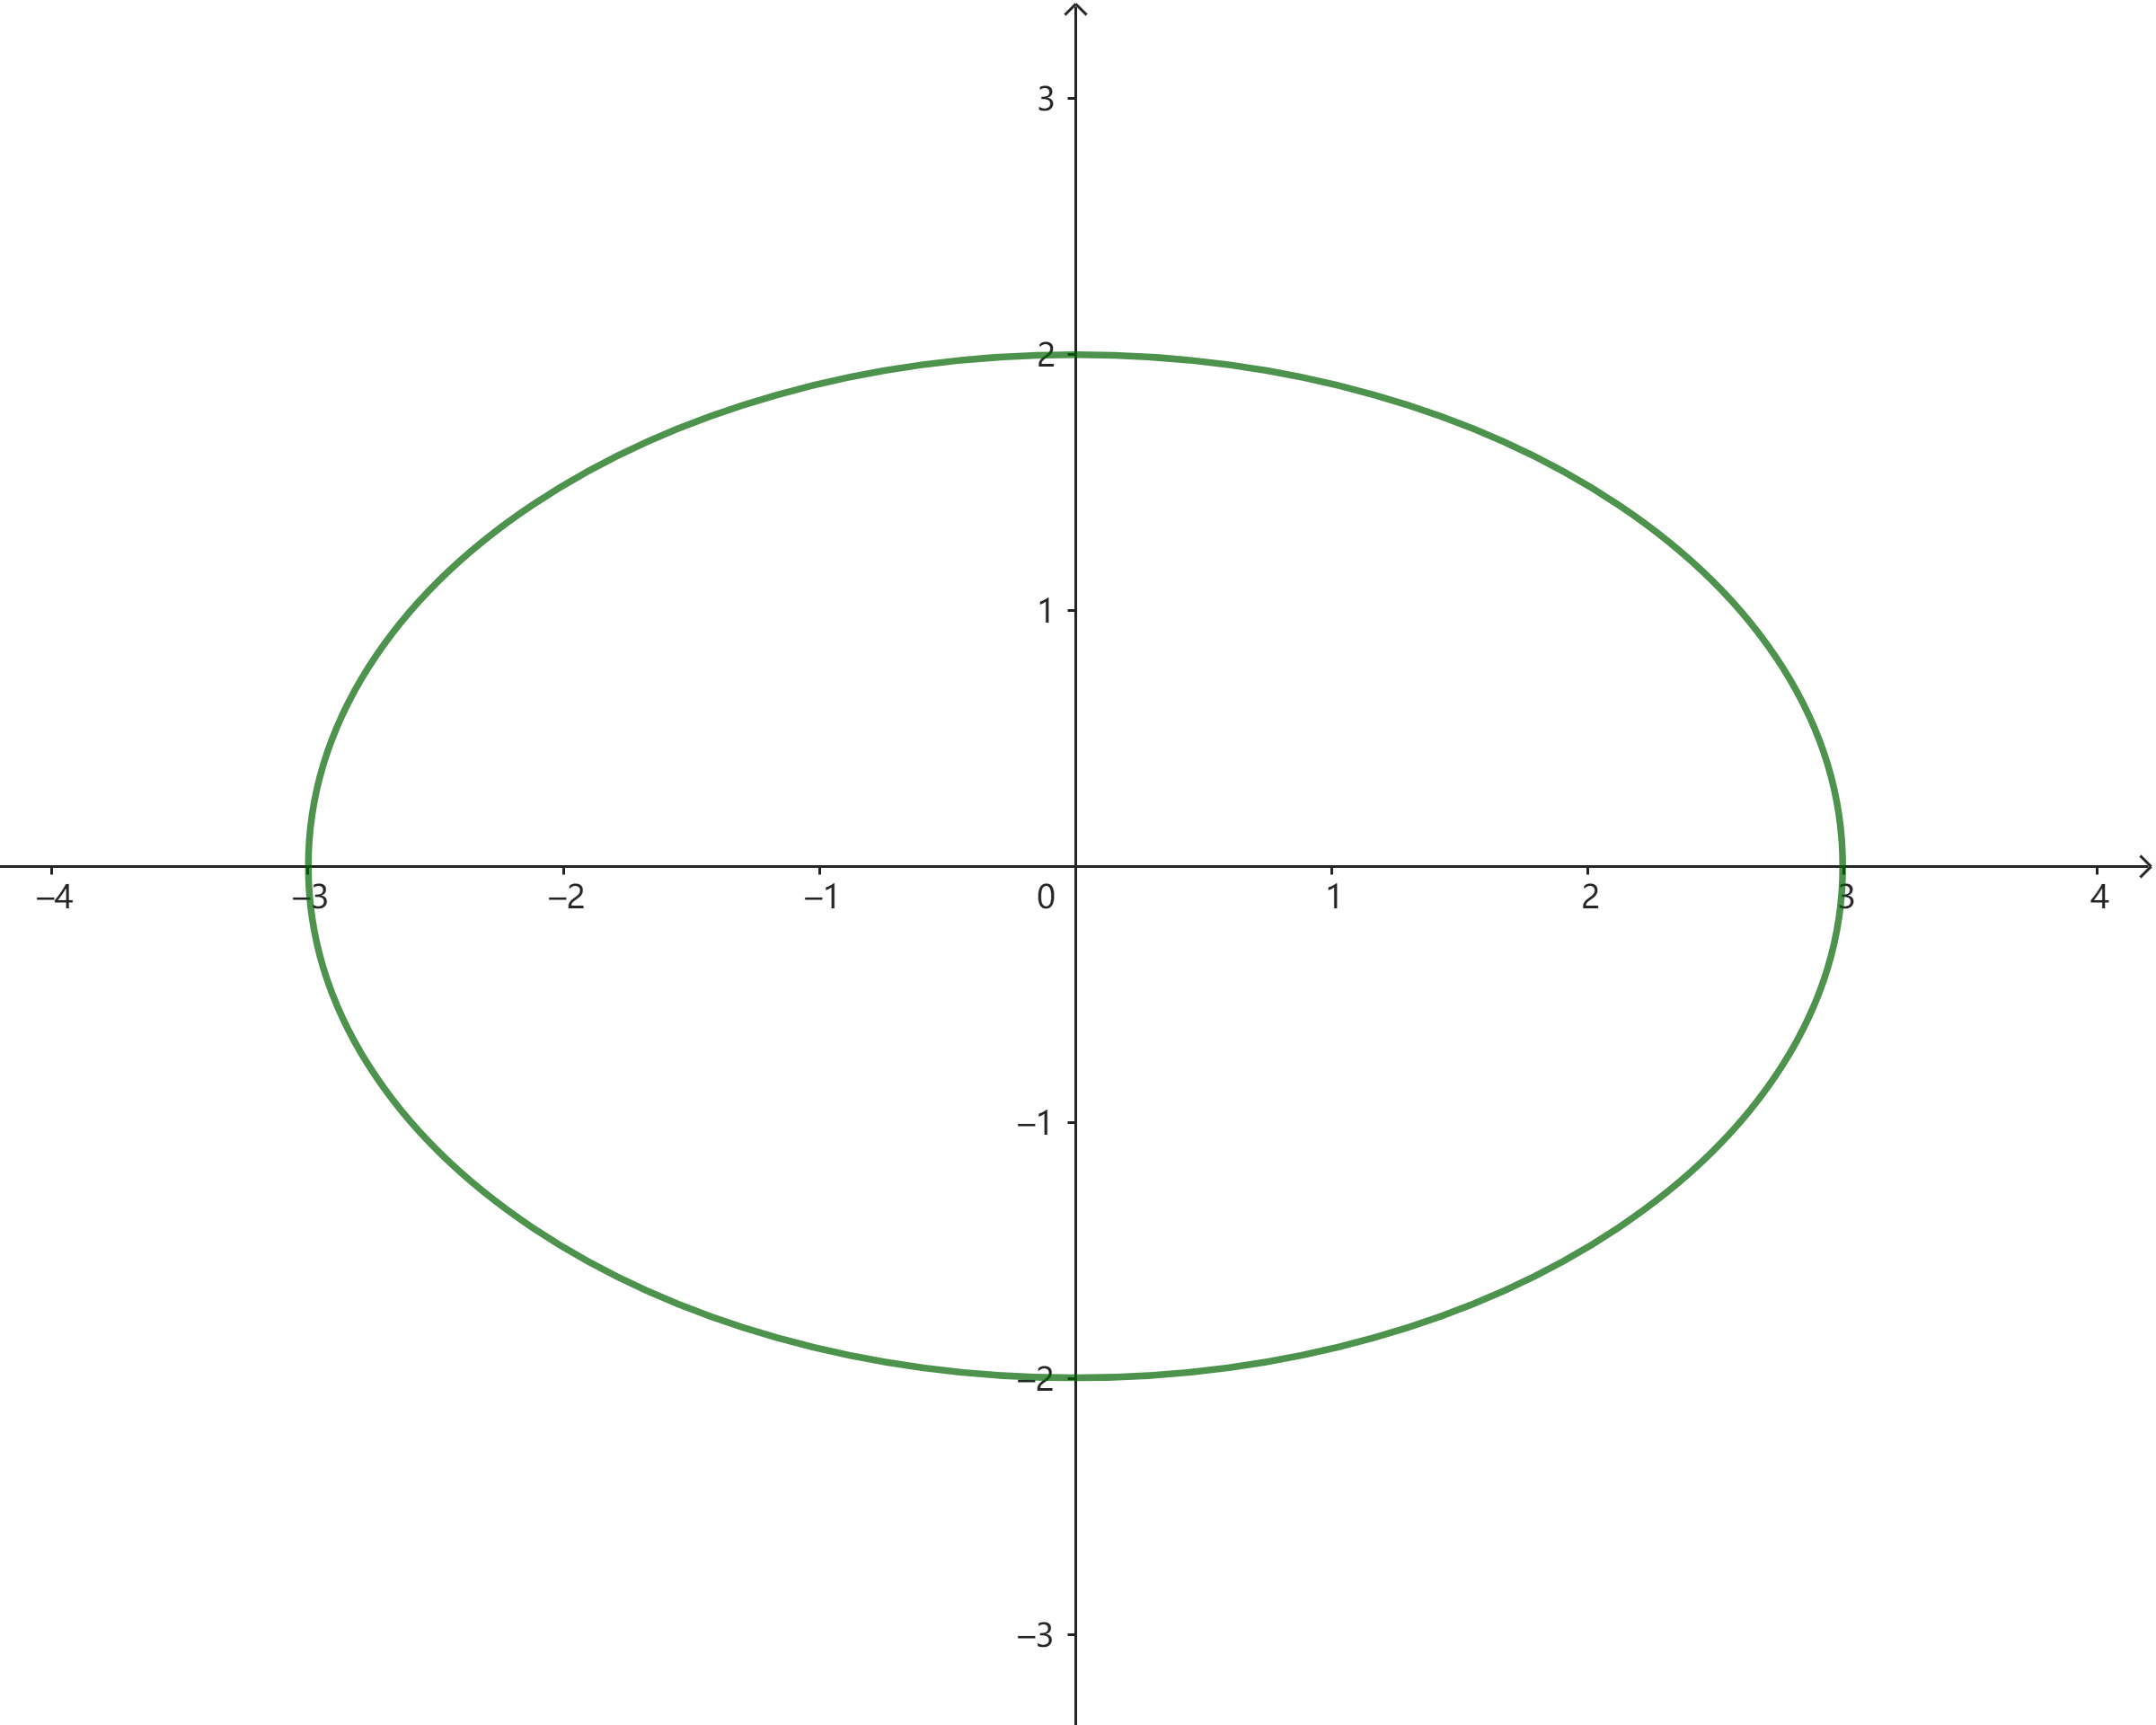
\includegraphics[width=0.3\textwidth]{tu/椭圆1.png}
\end{wrapfigure}

如果$AC > 0$,可以画出曲线如图。这样的曲线称为椭圆。典型的椭圆方程可以写为:
$$ \frac{x^2}{a^2} + \frac{y^2}{b^2} = 1 $$
其中$a,b>0$。

从这个方程来看,椭圆可以理解为圆经过$x$轴方向(或$y$轴方向)放缩得到。椭圆的曲线是闭合曲线。
椭圆上的点$(x,\,\,y)$总满足
$$ -a \leqslant x \leqslant a, \quad -b \leqslant y \leqslant b$$
这说明椭圆曲线是有界的。

% 双曲线例图(渐近线)
\begin{wrapfigure}[5]{r}{0.32\textwidth} %this figure will be at the right
    \vspace{-12pt}
    \flushright
    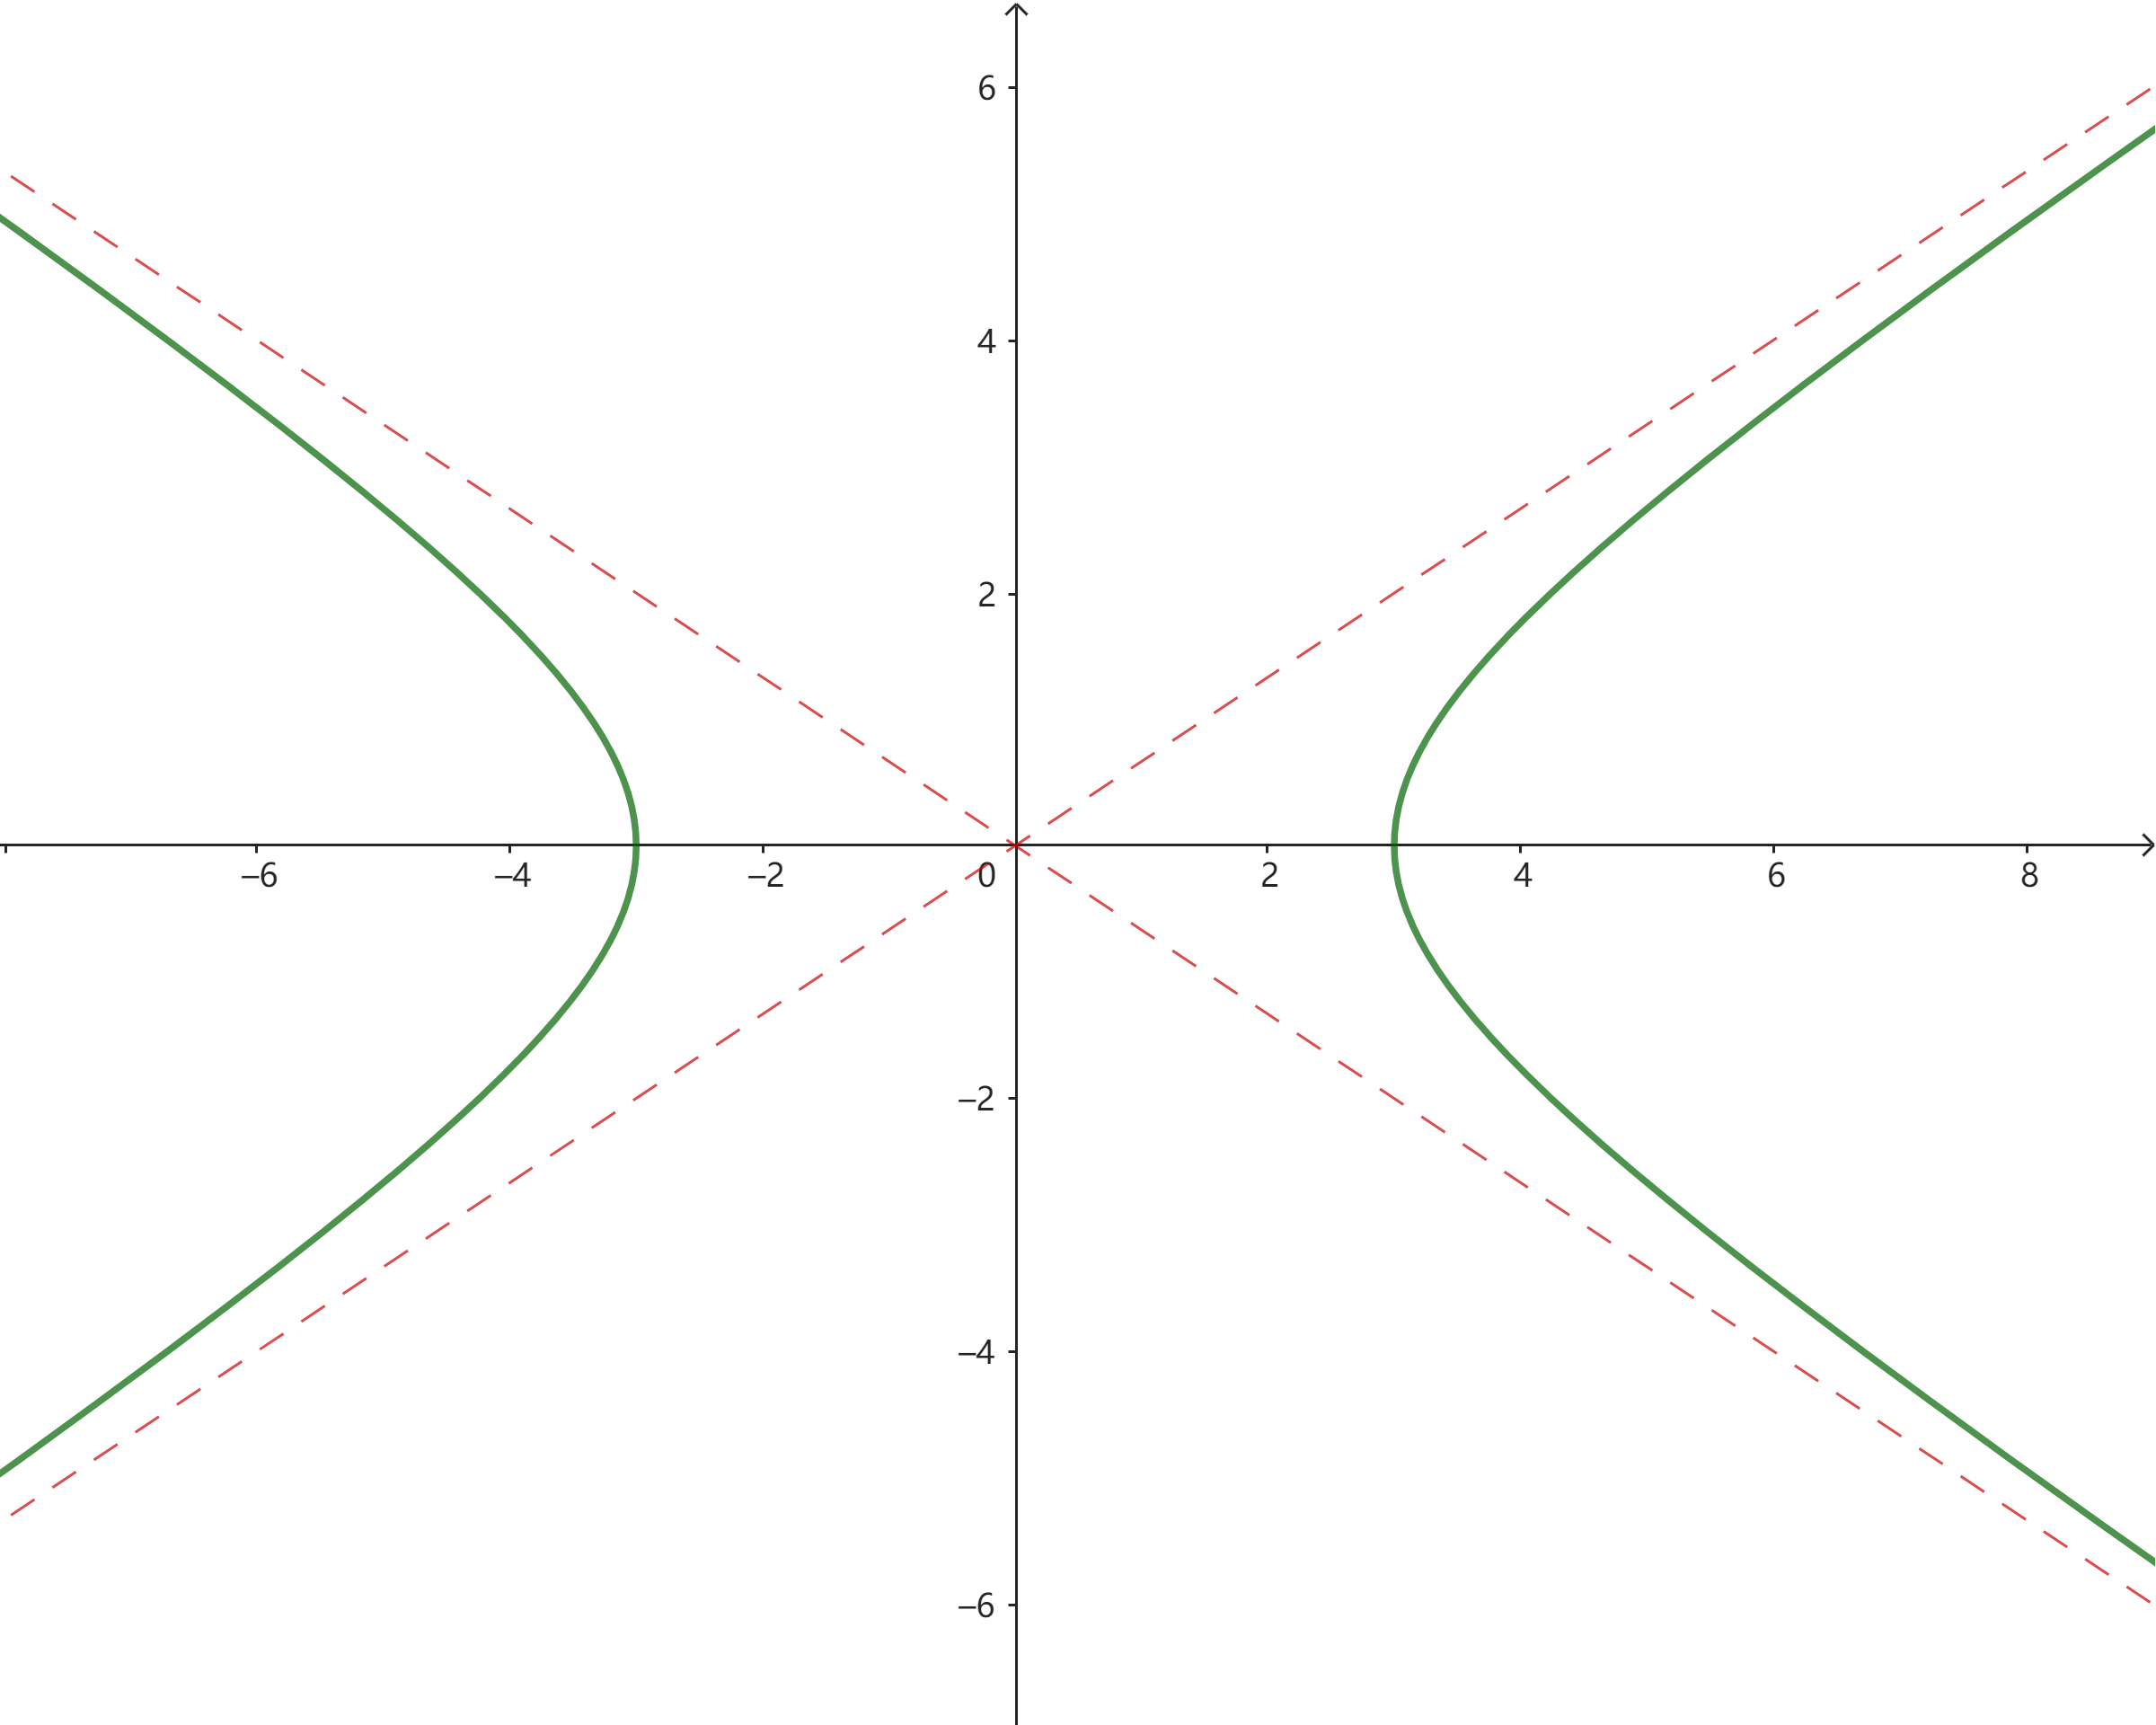
\includegraphics[width=0.3\textwidth]{tu/双曲线1.png}
\end{wrapfigure}

如果$B = 0$,$AC < 0$,可以画出曲线如图。这样的曲线称为双曲线。典型的双曲线方程可以写为:
$$ \frac{x^2}{a^2} - \frac{y^2}{b^2} = 1 \quad \mbox{(如右图)}$$
或
$$ - \frac{x^2}{a^2} + \frac{y^2}{b^2} = 1  \quad \mbox{(如左下图)} \qquad  \qquad  \qquad  \qquad \;\: \quad \phantom{123}$$
其中$a,b>0$。

\begin{wrapfigure}[5]{l}{0.32\textwidth} 
    \vspace{-28pt}
    \flushright
    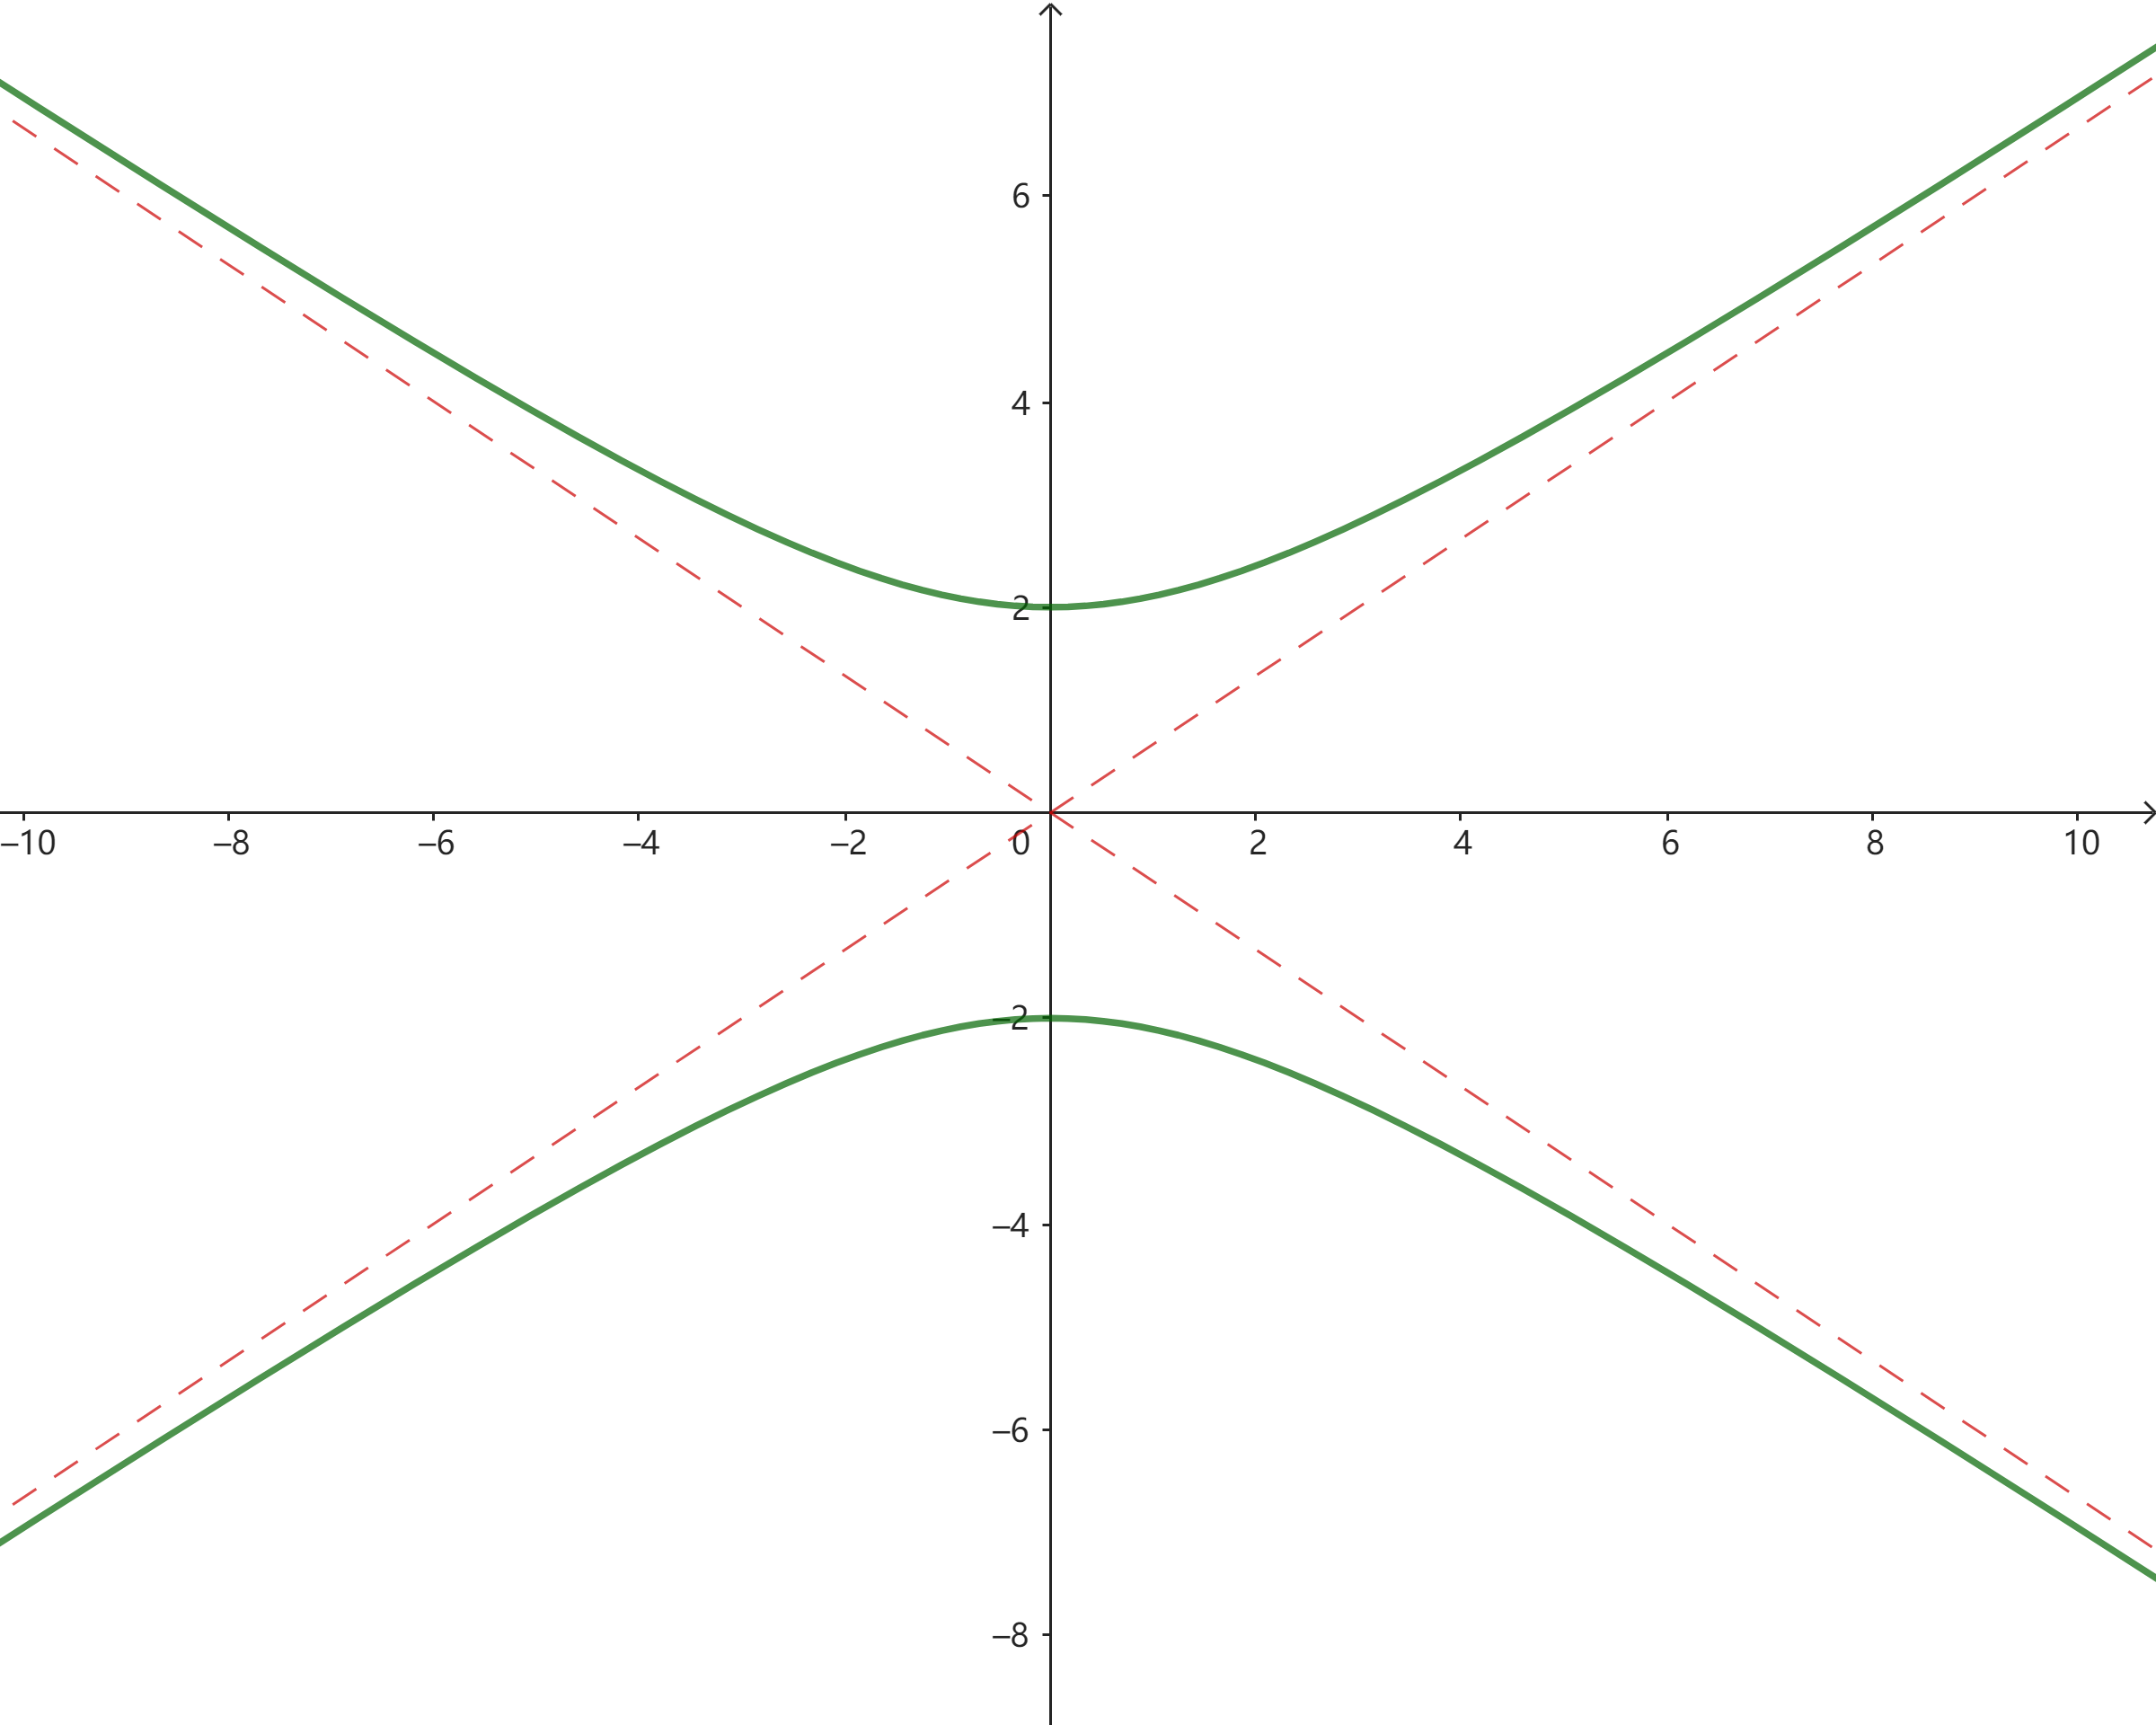
\includegraphics[width=0.3\textwidth]{tu/双曲线2.png}
\end{wrapfigure}

可以看到,双曲线由两个不相连的分支构成,一般按位置称为上下支或左右支。曲线不是闭合的,而是无界的,
关于$x$轴和$y$轴对称。
随着$x$趋于无穷,$y$也趋于无穷,反之亦然。而由于
$$ \phantom{123455}\qquad \qquad \qquad \qquad y^2 = \frac{b^2x^2}{a^2} \pm 1, $$
因此在$x$、$y$趋于无穷大时,
\begin{align*}
    y &= \pm \frac{b}{a} \cdot x \cdot \sqrt{1 \pm \frac{a^2}{b^2x^2}} \\ 
    &= \pm \frac{b}{a} \cdot x \cdot \left(1 \pm \frac{a^2}{b^2x^2}\right)^{\frac{1}{2}} \\
    &= \pm \frac{b}{a} \cdot x \cdot \left(1 \pm \frac{a^2}{2b^2x^2} + \olim{\frac{1}{x^2}} \right)\\
    &= \pm \frac{b}{a} \cdot x \pm \frac{a}{2bx} + \olim{\frac{1}{x}} \\
    &= \pm \frac{b}{a} \cdot x + \olim{1}.
\end{align*}

随着$x$、$y$逐渐增大,式子右边逐渐趋于$\displaystyle\pm \frac{b}{a} x$,
换句话说,$(x, \,\, y)$逐渐接近直线
$$ y = \pm \frac{b}{a}x. $$
我们把这两条过原点的直线(上图中的红色虚线)称为双曲线的\textbf{渐近线}。

% 抛物线例图
\begin{wrapfigure}[5]{r}{0.32\textwidth} %this figure will be at the right
    % \vspace{-30pt}
    \flushright
    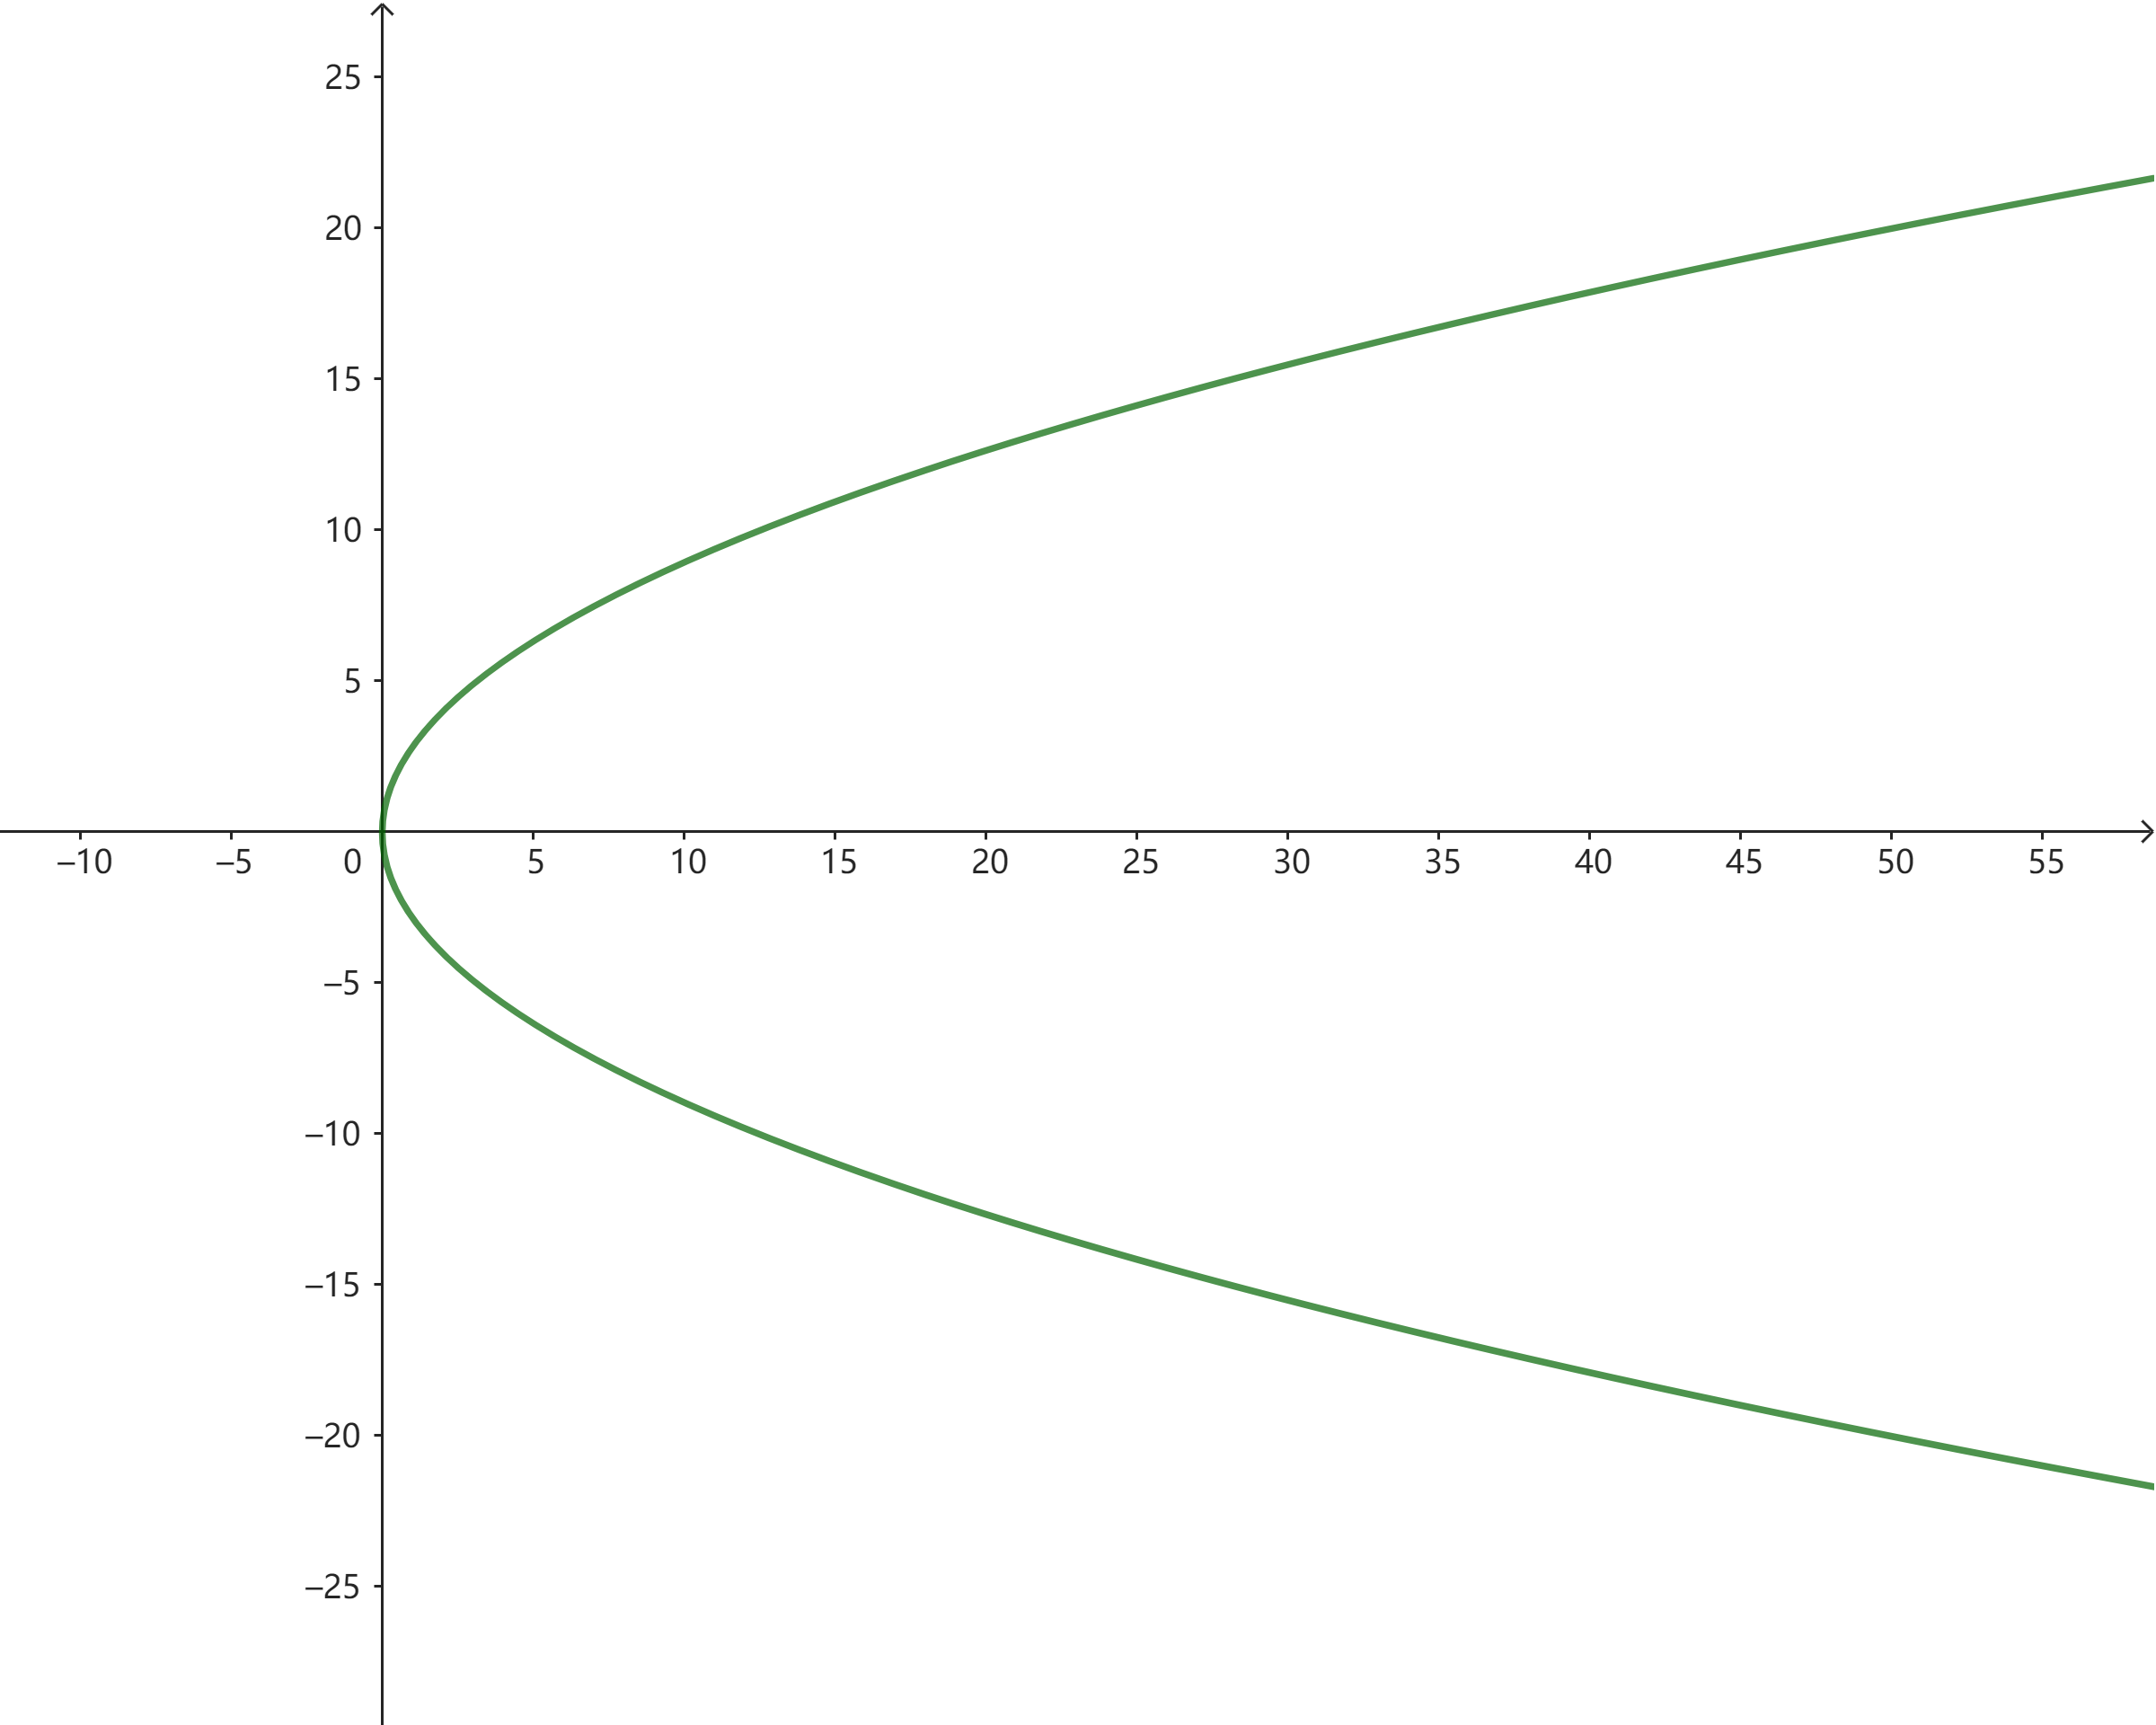
\includegraphics[width=0.3\textwidth]{tu/抛物线1.png}
\end{wrapfigure}

如果$AC = 0$,可以画出曲线如右图。这样的曲线称为抛物线。典型的抛物线方程可以写为:
$$ y^2 = 2px  \quad \mbox{(如右图)} $$
或
$$ x^2 = 2py  \quad \mbox{(如左下图)} \qquad  \qquad  \qquad  \qquad\;\;\; \phantom{123}$$
其中$p \neq 0$是描述抛物线的参数。

\begin{wrapfigure}[5]{l}{0.32\textwidth} %this figure will be at the right
    \vspace{-30pt}
    \flushright
    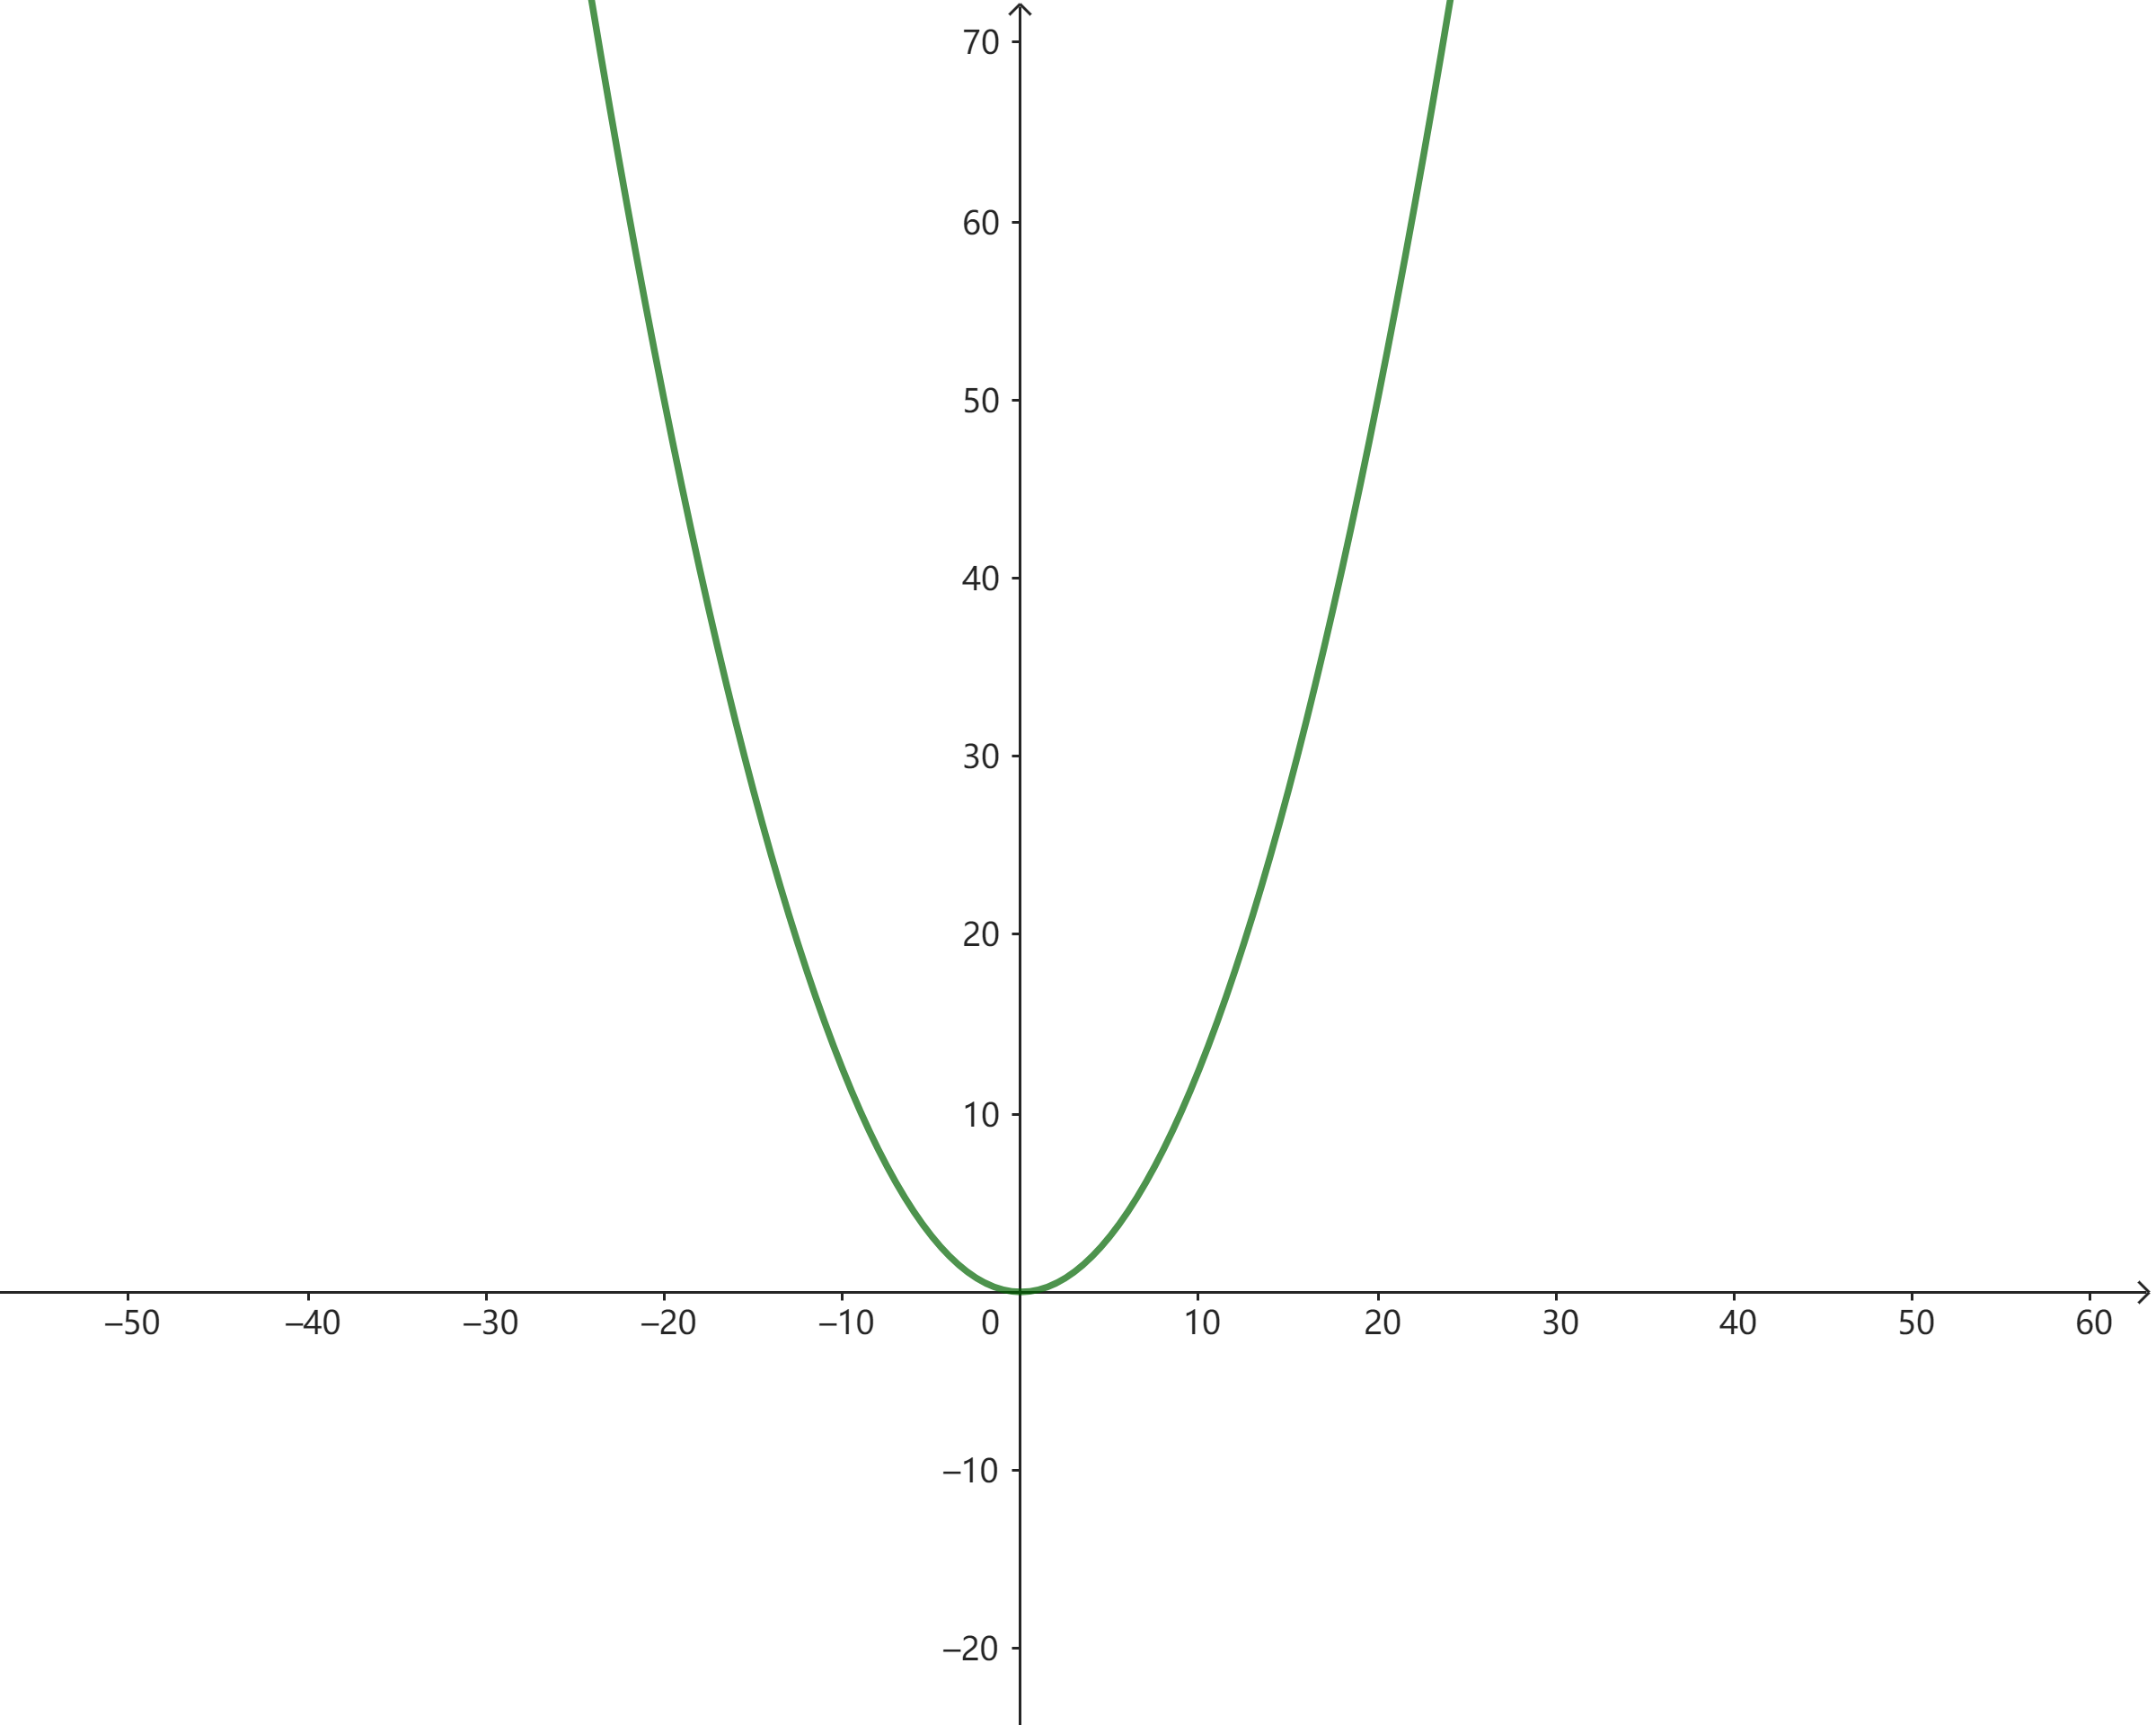
\includegraphics[width=0.3\textwidth]{tu/抛物线2.png}
\end{wrapfigure}

抛物线就是二次函数的曲线。按开口方向,抛物线可分为上下左右四类。它不是闭合曲线,也不是有界曲线,
恰有一条对称轴,与开口方向平行。

这三类曲线称为二次曲线。我们接下来会看到,一般的二次曲线要么是这三类曲线之一,要么是直线、点或空集(称为退化情形)。

考虑一般的二次曲线:
$$ Ax^2 + Bxy + Cy^2 + Dx + Ey + F = 0.$$

对于$B = 0$的情况,如果$AC\neq 0$,将曲线按向量$\displaystyle\left(-\frac{D}{2A},\,\,-\frac{E}{2C}\right)$平移,
就得到:
$$ Ax^2 + Cy^2 + F' = 0.$$
其中$F' = F - \frac{D^2}{4A} - \frac{E^2}{4C}$。两边除以$AC$并移项,得到:
$$ \frac{x^2}{C} + \frac{y^2}{A} = -\frac{F'}{AC}.$$
因此,根据$A$、$C$、$F'$的正负性,可以判断它或者是椭圆($A,C$同号,$A,F'$异号),
或者是双曲线($A,C$异号,$F' \neq 0$),或者是两条过原点直线($F' = 0$),或者是空集或单点集($A,C,F'$同号)。

如果$B = 0$,$A,C$中恰有一个为零,不妨设$A = 0$,则方程变为:
$$ Cy^2 + Dx + Ey + F = 0.$$

如果$D = 0$,则曲线方程变为关于$y$的二次方程,图像为$y = y_0$类型的水平线,条数等于方程实根的个数。

如果$D\neq 0$,按$\displaystyle\left(\frac{E^2 - 4CF}{4CD},\,\,-\frac{E}{2C}\right)$平移,就得到:
$$ Cy^2 = -Dx. $$
即
$$ y^2 = -\frac{D}{C}x. $$
因此曲线为抛物线。$C=0$而$A\neq 0$的情形也类同。

如果$B\neq 0$,我们希望通过某种变换,将方程转化为$B = 0$,即$xy$系数为$0$的情况。我们采用旋转变换。将坐标系逆时针旋转$\theta$角,
对应的旋转矩阵为:
$$
\begin{bmatrix}
    \cos{\theta} & -\sin{\theta} \\
    \sin{\theta} & \cos{\theta} 
\end{bmatrix}
$$
原坐标系中点$(x,\,\,y)$在新坐标系中坐标$(u,\,\,v)$满足:
$$
\begin{bmatrix}
    x \\ y
\end{bmatrix}
=
\begin{bmatrix}
    \cos{\theta} & -\sin{\theta} \\
    \sin{\theta} & \cos{\theta} 
\end{bmatrix}
\begin{bmatrix}
    u \\ v
\end{bmatrix}
= 
\begin{bmatrix}
    \cos{(\theta)}u - \sin{(\theta)}v \\ \sin{(\theta)}u + \cos{(\theta)}v
\end{bmatrix}
$$

% 双曲线、椭圆旋转后平移得到标准型

代入曲线方程,得到关于新坐标$(u,\,\,v)$的二次曲线方程,其中二次项为:
\begin{align*}
    Ax^2 + Bxy + Cy^2 &= A(\cos{(\theta)}u - \sin{(\theta)}v)^2 \\
    &\quad + B(\cos{(\theta)}u - \sin{(\theta)}v)(\sin{(\theta)}u + \cos{(\theta)}v) \\
    &\quad + C(\sin{(\theta)}u + \cos{(\theta)}v)^2 \\
    &= (A\cos^2{\theta} + B\cos{\theta}\sin{\theta} + C\sin^2{\theta})u^2 \\
    &\quad + (A\sin^2{\theta} - B\cos{\theta}\sin{\theta} + C\cos^2{\theta})v^2 \\
    &\quad + 2\cos{\theta}\sin{\theta}(C - A) + B(\cos^2{\theta} - \sin^2{\theta})uv
\end{align*}
$uv$的系数为:
$$ (C - A)\sin{(2\theta)} + B\cos{(2\theta)} $$
我们希望它等于$0$。

根据假设,$B\neq 0$。
如果$A = C$,那么取$\theta = \frac{\pi}{4}$即可。这时$u^2$、$v^2$的系数分别为
$$ A + \frac{B}{2}, \qquad A - \frac{B}{2}. $$
计算两者乘积,可以发现,两者同号(异号)当且仅当$4AC - B^2$大于(小于)零。

如果$A\neq C$,那么取
$$\theta = \theta_c = \frac{1}{2} \arctan{\frac{B}{A - C}},$$

% \begin{align*}
%     \cos{(2\theta_c)} &= \frac{A - C}{\Delta} \\
%     \sin{(2\theta_c)} &= \frac{B}{\Delta}  \\
%     \Delta &= \sqrt{B^2 + (A - C)^2}
% \end{align*}

% \begin{align*}
%     &\;A\cos^2{(\theta_c)} + B\cos{\theta}\sin{\theta} + C\sin^2{\theta} \\
%    =&\;\frac{A+C}{2} + \frac{A-C}{2}\cos{(2\theta_c)} + \frac{B}{2}\sin{(\theta_c)} \\
%    =&\;\frac{A+C}{2} + \frac{A-C}{2}\frac{A - C}{\Delta} + \frac{B}{2}\frac{B}{\Delta} \\
%    =&\;\frac{A+C}{2} + \frac{1}{2\Delta}\left((A - C)^2 + B^2\right) \\
%    =&\;\frac{A+C}{2} + \frac{\Delta^2}{2\Delta} \\
%    =&\;\frac{A+C}{2} + \frac{\Delta}{2} \\
% \end{align*}

则$uv$的系数为$0$。这时$u^2$、$v^2$的系数分别为:
$$ \frac{A+C}{2} + \frac{\sqrt{B^2 + (A - C)^2}}{2}, \qquad \frac{A+C}{2} - \frac{\sqrt{B^2 + (A - C)^2}}{2}. $$
计算两者乘积,可以发现,两者同号(异号)仍然当且仅当$4AC - B^2$大于(小于)零。

综上所述,任何二次曲线都可以通过旋转和平移,转变为典型的三类曲线之一,或退化情形。
也就是说,任何二次曲线,只要是“弯的”,就必然是椭圆、双曲线,或抛物线\footnote{我们约定圆是椭圆的特殊情形。}。
对于一般的二次曲线,我们可以用二次项的系数来直接判定它属于哪一类。
\begin{itemize}
    \item 如果$B^2<4AC$,那么二次曲线为\textbf{椭圆类型}(椭圆、圆或退化情形);
    \item 如果$B^2>4AC$,那么二次曲线为\textbf{双曲类型}(双曲线或退化情形);
    \item 如果$B^2=4AC$,那么二次曲线为\textbf{抛物线型}(抛物线或退化情形)。
\end{itemize}

\begin{sk}
    \mbox{} \\
    \indent 1. 
\end{sk}

\begin{xt}
    \mbox{} \\
    \indent 1. 
    
\end{xt}

\section{二次曲线的性质}

让我们来研究三类二次曲线:椭圆、双曲线、抛物线。历史上,数学家是通过直观的性质来发现并定义它们的。

首先,二次曲线可以通过到定点(定直线)的距离定义。

设配备直角坐标系$xOy$的平面上有两点$F_1:(-c,\,\,0)$和$F_2:(c,\,\,0)$。

考虑到这两点距离之和为$2a$的点的轨迹($a\geqslant c$)。

设平面上有点$P(x, \,\,y)$,它到$F_1$、$F_2$距离之和为$2a$,可列出方程:
$$ \sqrt{(x + c)^2 + y^2} + \sqrt{(x - c)^2 + y^2} = 2a.$$
移项平方:
\begin{align*}
    (x + c)^2 + y^2 &= (2a - \sqrt{(x - c)^2 + y^2})^2 = 4a^2 - 4a\sqrt{(x - c)^2 + y^2} + (x - c)^2 + y^2 \\
    4a\sqrt{(x - c)^2 + y^2} &= 4a^2 - 4cx.
\end{align*}
再平方,得到:
\begin{align*}
    (x - c)^2 + y^2 &= \left(a - \frac{cx}{a}\right)^2 \\
    (1 - \frac{c^2}{a^2})x^2 + y^2 &= a^2 - c^2.
\end{align*}
如果$a = c$,则得到$y = 0$,从而$-c \leqslant x \leqslant c$,轨迹为线段$F_1F_2$。

如果$a > c$,则得到:
$$ \frac{x^2}{a^2} + \frac{y^2}{a^2 - c^2} = 1.$$
记$b = \sqrt{a^2 - c^2}$,则得到$P$属于椭圆:
$$ \frac{x^2}{a^2} + \frac{y^2}{b^2} = 1.$$

反之,设$P$为椭圆上的点,则它到$F_1$、$F_2$的距离之和为:
\begin{align*}
    &\;\sqrt{(x + c)^2 + y^2} + \sqrt{(x - c)^2 + y^2}  \\
    =&\;\sqrt{(x + c)^2 + a^2 - c^2\left(1 - \frac{x^2}{a^2}\right)} + \sqrt{(x - c)^2 + a^2 - c^2\left(1 - \frac{x^2}{a^2}\right)} \\
    =&\;\sqrt{\frac{c^2x^2}{a^2} + 2cx + a^2} + v\sqrt{\frac{c^2x^2}{a^2} - 2cx + a^2} \\
    =&\; \left|a + \frac{cx}{a}\right| + \left|a - \frac{cx}{a}\right|
\end{align*}
由于$|x| \leqslant a$,所以$\displaystyle\left|\frac{cx}{a}\right| \leqslant c \leqslant a$,于是距离之和为
$2a$。

综上所述,$a>c$时,轨迹为椭圆。

也就是说,椭圆可以定义为平面上到两点距离之和为定值的点的轨迹。

\begin{figure}[h] 
    % \vspace{-4pt}
    \centering
    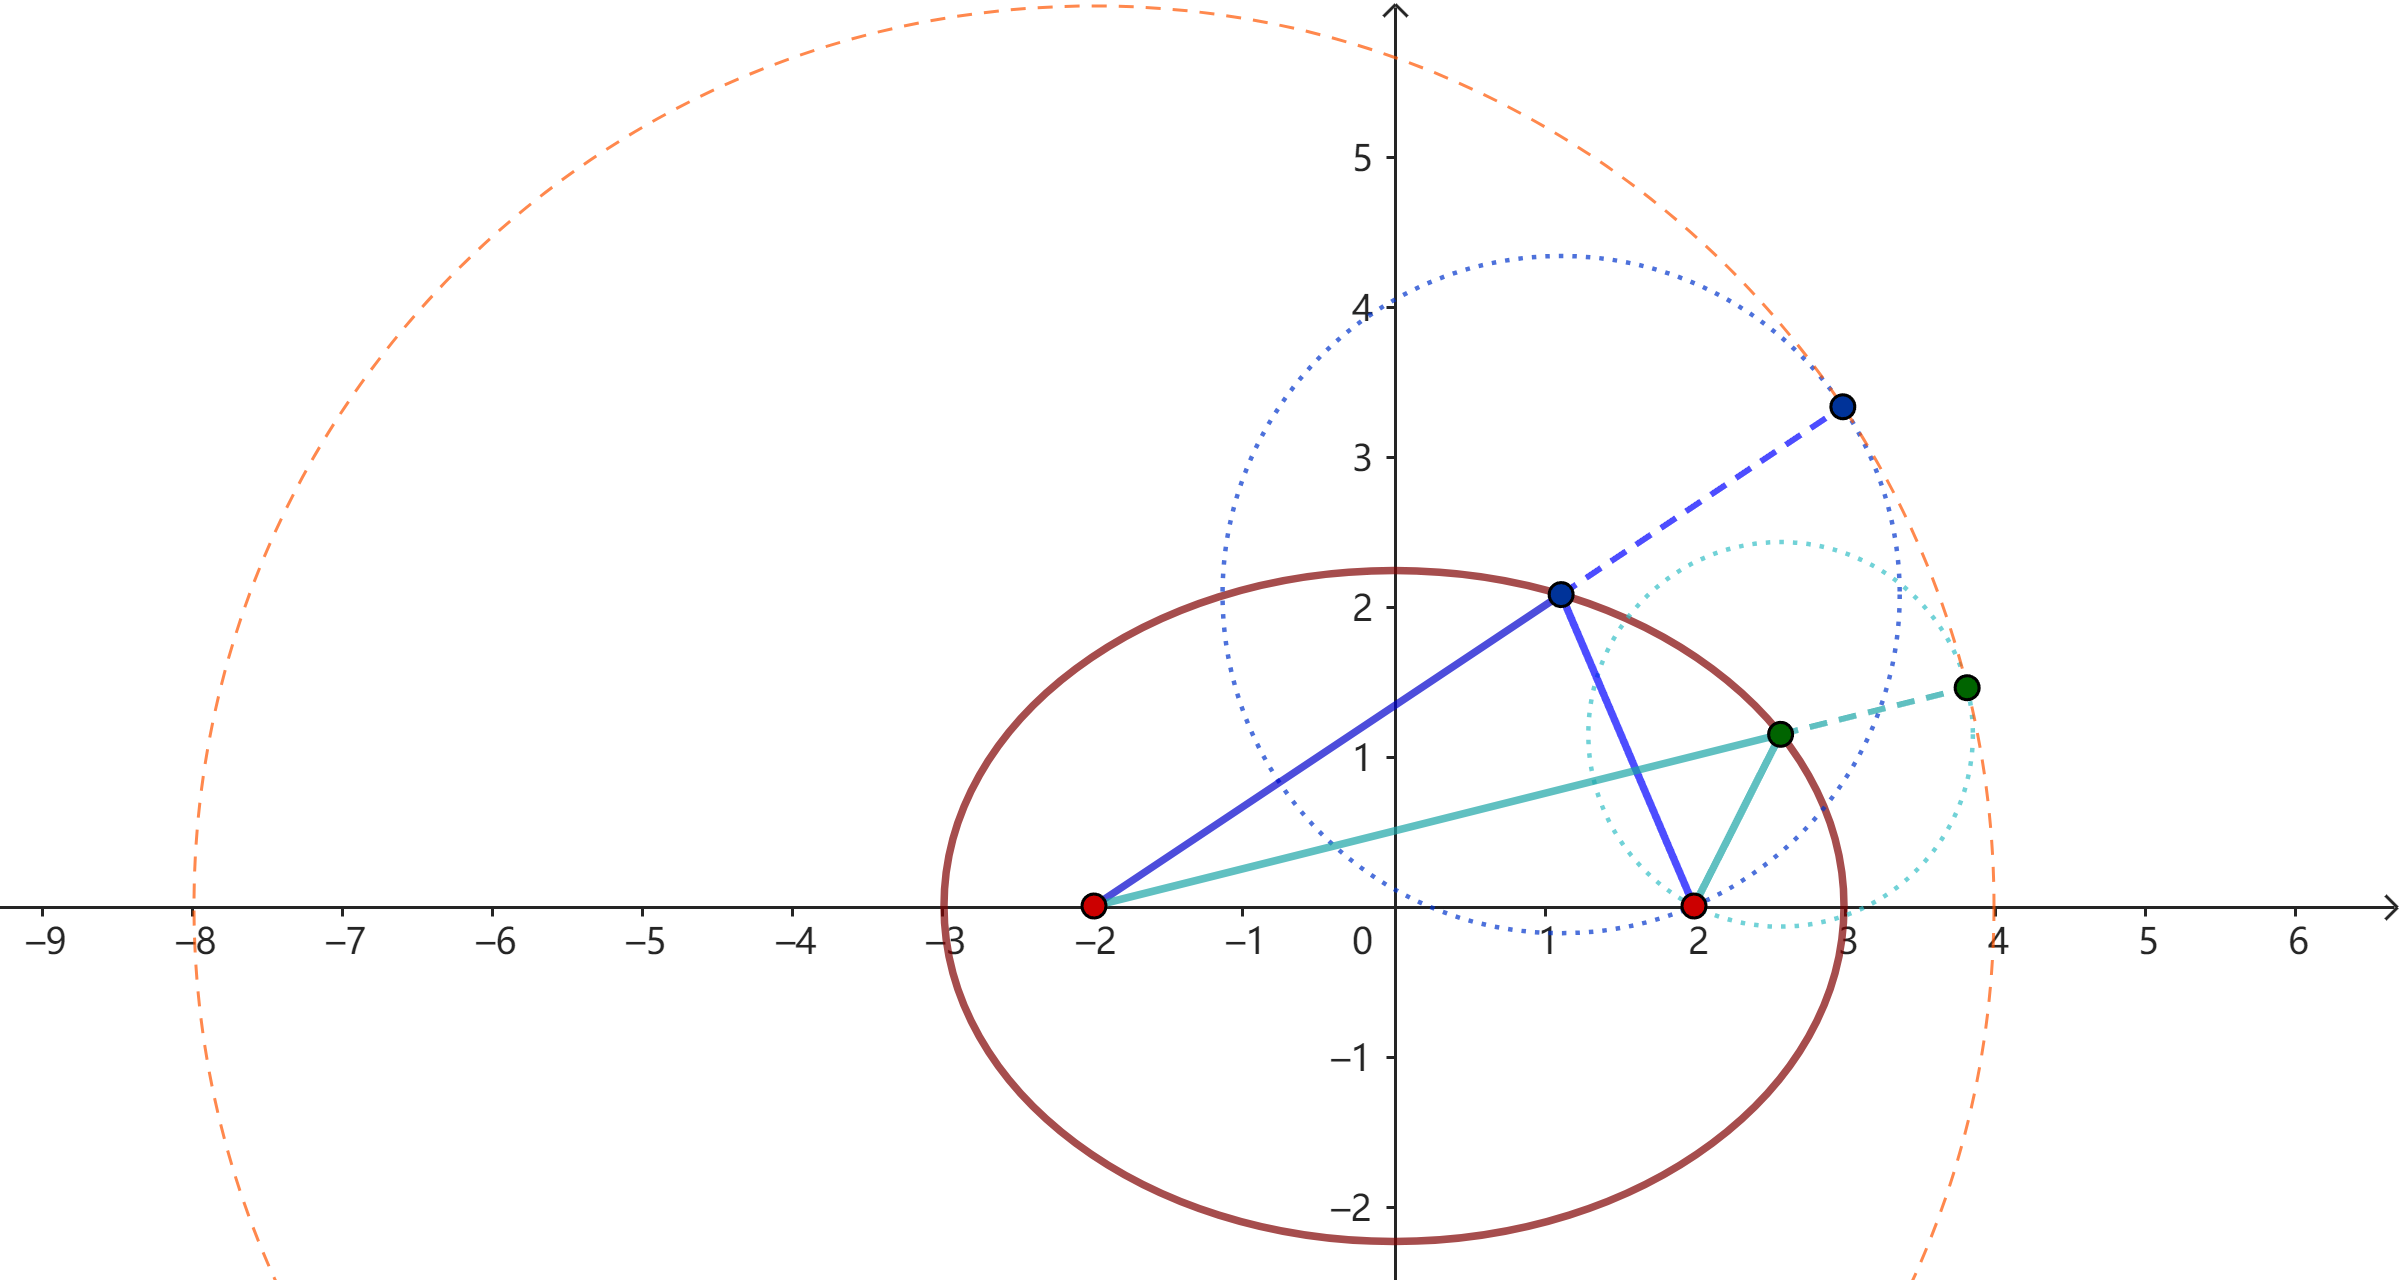
\includegraphics[width=0.8\textwidth]{tu/椭圆第一定义.png}
    \caption*{\texttt{到两点距离之和为定值的点的轨迹}}
\end{figure}

我们称$F_1$、$F_2$为椭圆的\textbf{焦点},$F_1F_2$中点为\textbf{椭圆中心},椭圆的\textbf{焦距}为$2c$。
椭圆与$x$轴、$y$轴的交点距离称为它的\textbf{长轴}和\textbf{短轴}。长轴、短轴分别为$2a$、$2b$(较大者为长轴)。

焦距和长轴之比$\displaystyle e =\frac{c}{a}$称为椭圆的\textbf{离心率}。离心率介于$0$和$1$之间。离心率越大,椭圆越狭长。离心率为$0$时,两焦点重合,椭圆就是圆。

再考虑到这两点距离之差为$2a$的点的轨迹($a\leqslant c$)。

设平面上有点$P(x, \,\,y)$,它到$F_1$、$F_2$距离之差为$2a$,可列出方程:
$$ \left|\sqrt{(x + c)^2 + y^2} - \sqrt{(x - c)^2 + y^2}\right| = 2a.$$
同上解得:
\begin{align*}
    \left(1 - \frac{c^2}{a^2}\right)x^2 + y^2 &= a^2 - c^2.
\end{align*}
如果$a = c$,则得到$y = 0$,从而$x \leqslant -c$或$x \geqslant c$,轨迹为$F_1$、$F_2$向$x$轴两方的射线。

如果$a < c$,则得到:
$$ \frac{x^2}{a^2} - \frac{y^2}{c^2 - a^2} = 1.$$
记$b = \sqrt{c^2 - a^2}$,则得到$P$属于双曲线:
$$ \frac{x^2}{a^2} - \frac{y^2}{b^2} = 1.$$

反之,设$P$为双曲线上的点,则它到$F_1$、$F_2$的距离之差为:
\begin{align*}
    &\;\left|\sqrt{(x + c)^2 + y^2} - \sqrt{(x - c)^2 + y^2}\right|  \\
    =&\; \Bigg|\left|a + \frac{cx}{a}\right| - \left|a - \frac{cx}{a}\right|\Bigg|
\end{align*}
由于$|x| \geqslant a$,$x \geqslant a$或$x \leqslant -a$。

$x \leqslant -a$时,$\frac{cx}{a} < x \leqslant -a$,所以$\left|a + \frac{cx}{a}\right| = -\frac{cx}{a} - a$,
$\left|a - \frac{cx}{a}\right| = a - \frac{cx}{a}$,于是距离之差为$2a$。

$x \geqslant a$时,$\frac{cx}{a} > x \geqslant a$,所以$\left|a - \frac{cx}{a}\right| = \frac{cx}{a} - a$,
$\left|a + \frac{cx}{a}\right| = a + \frac{cx}{a}$,于是距离之差为$2a$。

所以距离之差总是$2a$。综上,平面上到两点距离之差为定值的点的轨迹是双曲线。以上两种情况分别对应双曲线的左右两支。
双曲线同样定义焦点、焦距、交点、中心和离心率$\displaystyle e =\frac{c}{a}$。$2a$、$2b$分别称为\textbf{实轴}、\textbf{虚轴}。

双曲线的离心率$e$大于$1$。离心率越大,双曲线两支越靠近,各自的开口越宽。

\begin{figure}[h] 
    % \vspace{-4pt}
    \centering
    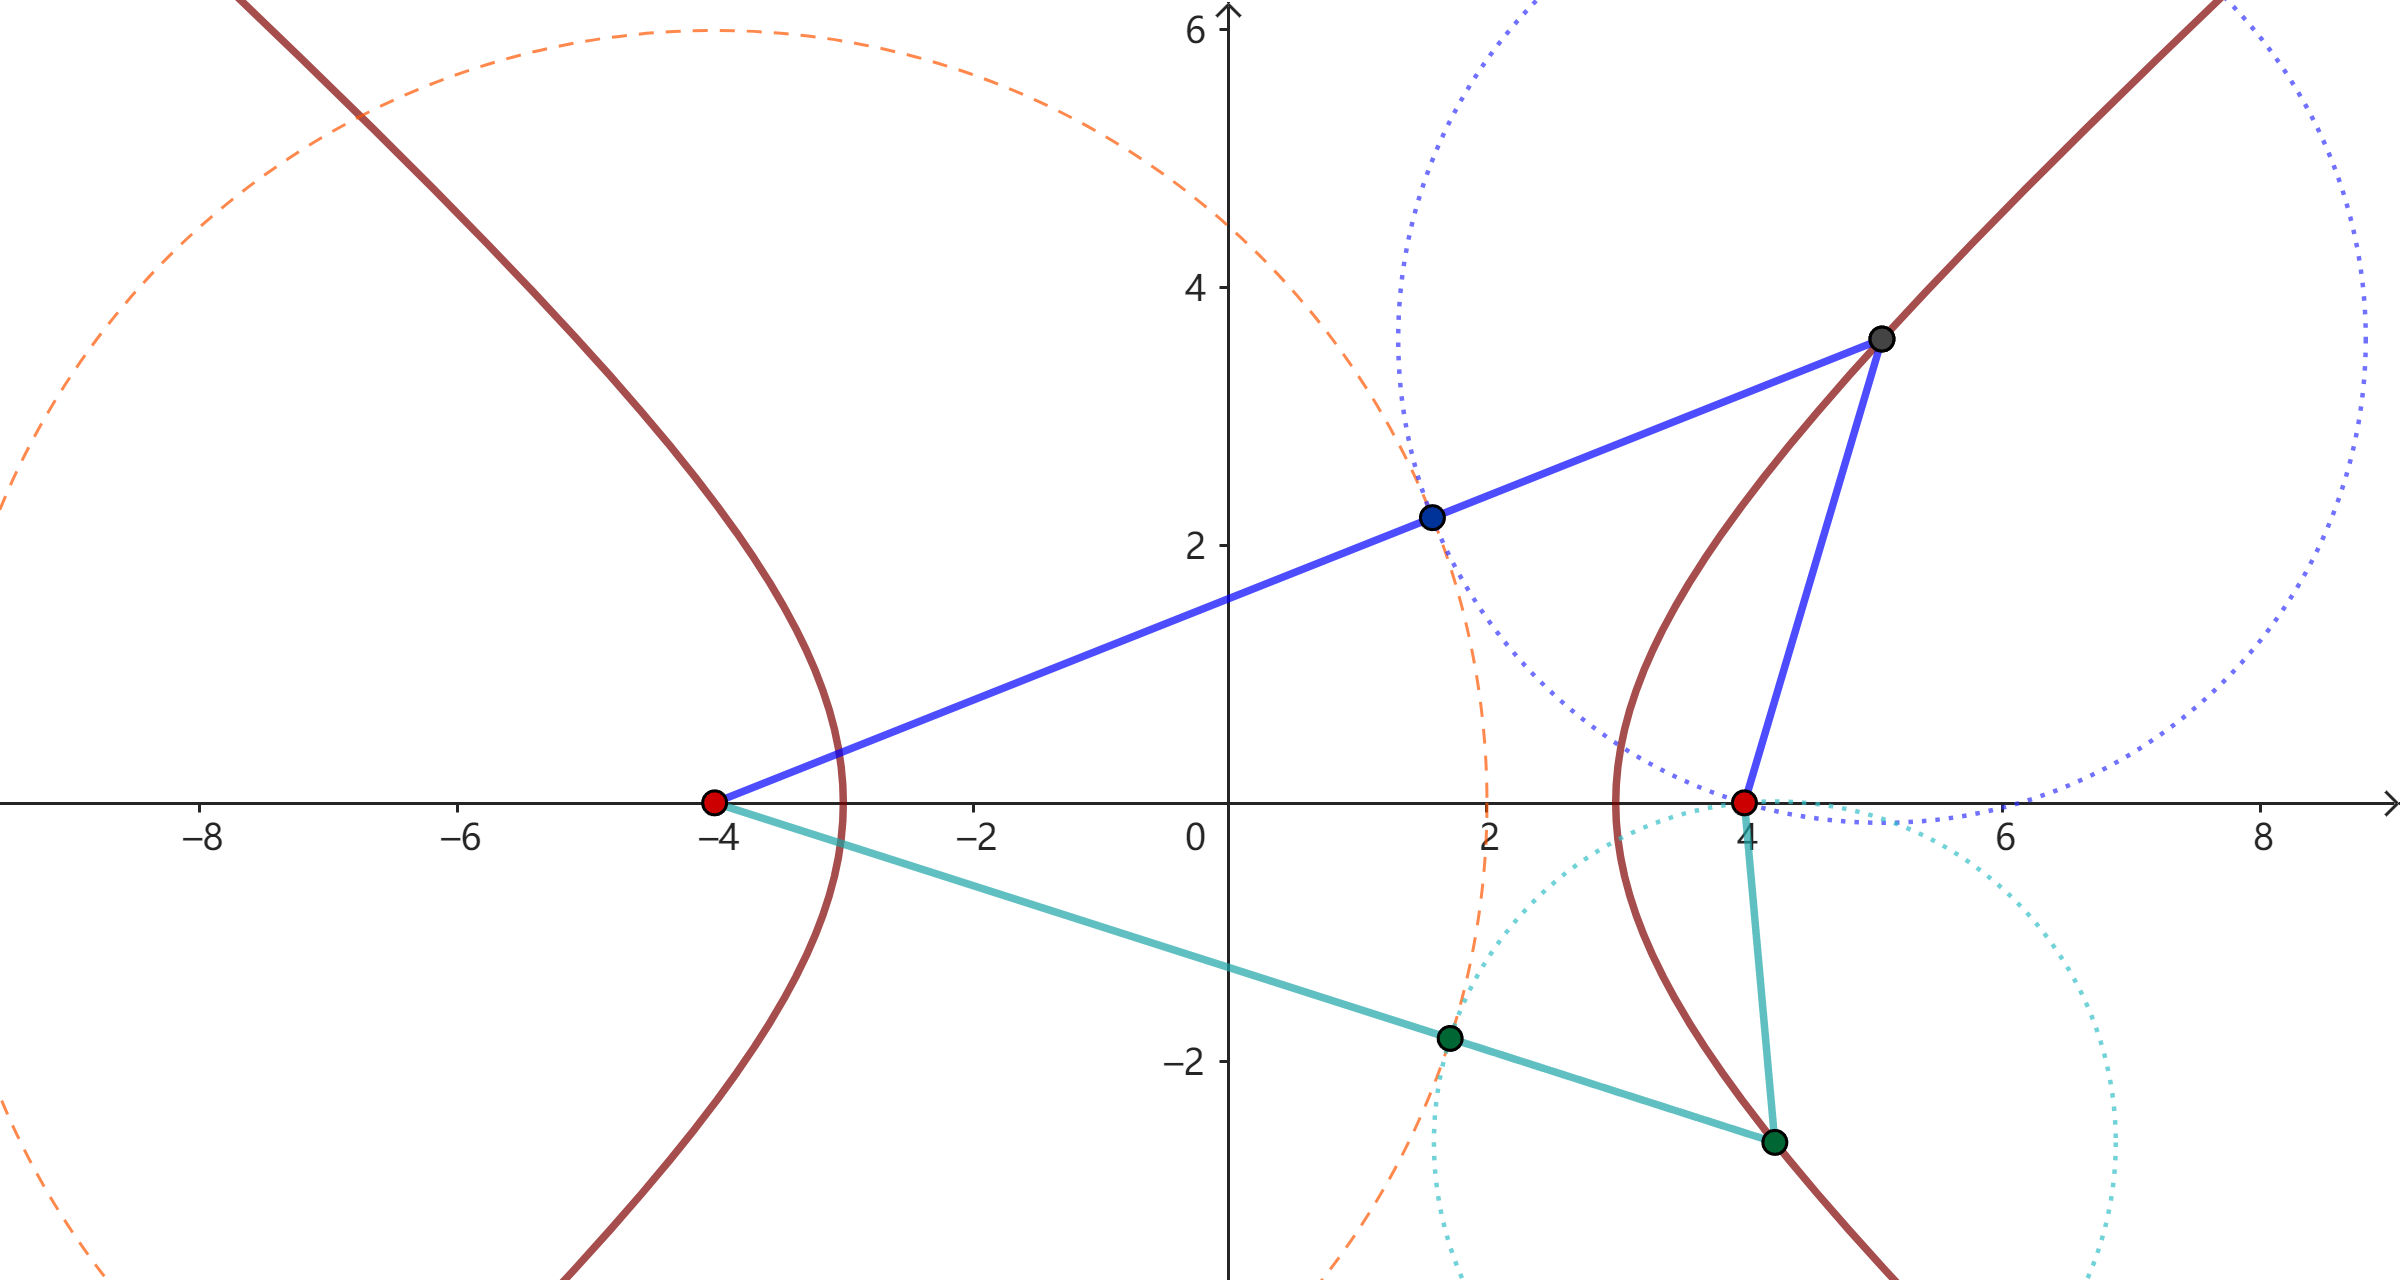
\includegraphics[width=0.8\textwidth]{tu/双曲线第一定义.png}
    \caption*{\texttt{到两点距离之差为定值的点的轨迹}}
\end{figure}

最后考虑到$F_2$和直线$x + c = 0$距离相等的点的轨迹。

设平面上有点$P(x, \,\,y)$,它到$F_2$和直线$x + c = 0$距离相等,可列出方程:
$$ \left|x + c\right| = \sqrt{(x - c)^2 + y^2}.$$
解得$P$属于抛物线:
$$ y^2 = 4cx.$$

反之,设$P$为抛物线上的点,则它到$F_2$的距离为:
\begin{align*}
    \sqrt{(x - c)^2 + y^2} &= \sqrt{(x - c)^2 + 4cx} = |x + c|.
\end{align*}
等于到直线$x + c = 0$的距离。

综上,轨迹为抛物线$ y^2 = 4cx$。抛物线是平面上到定点和定直线距离相等的点的轨迹。
$F_2$称为抛物线的\textbf{焦点}。$x + c = 0$称为抛物线的\textbf{准线}。

\begin{figure}[h] 
    % \vspace{-4pt}
    \centering
    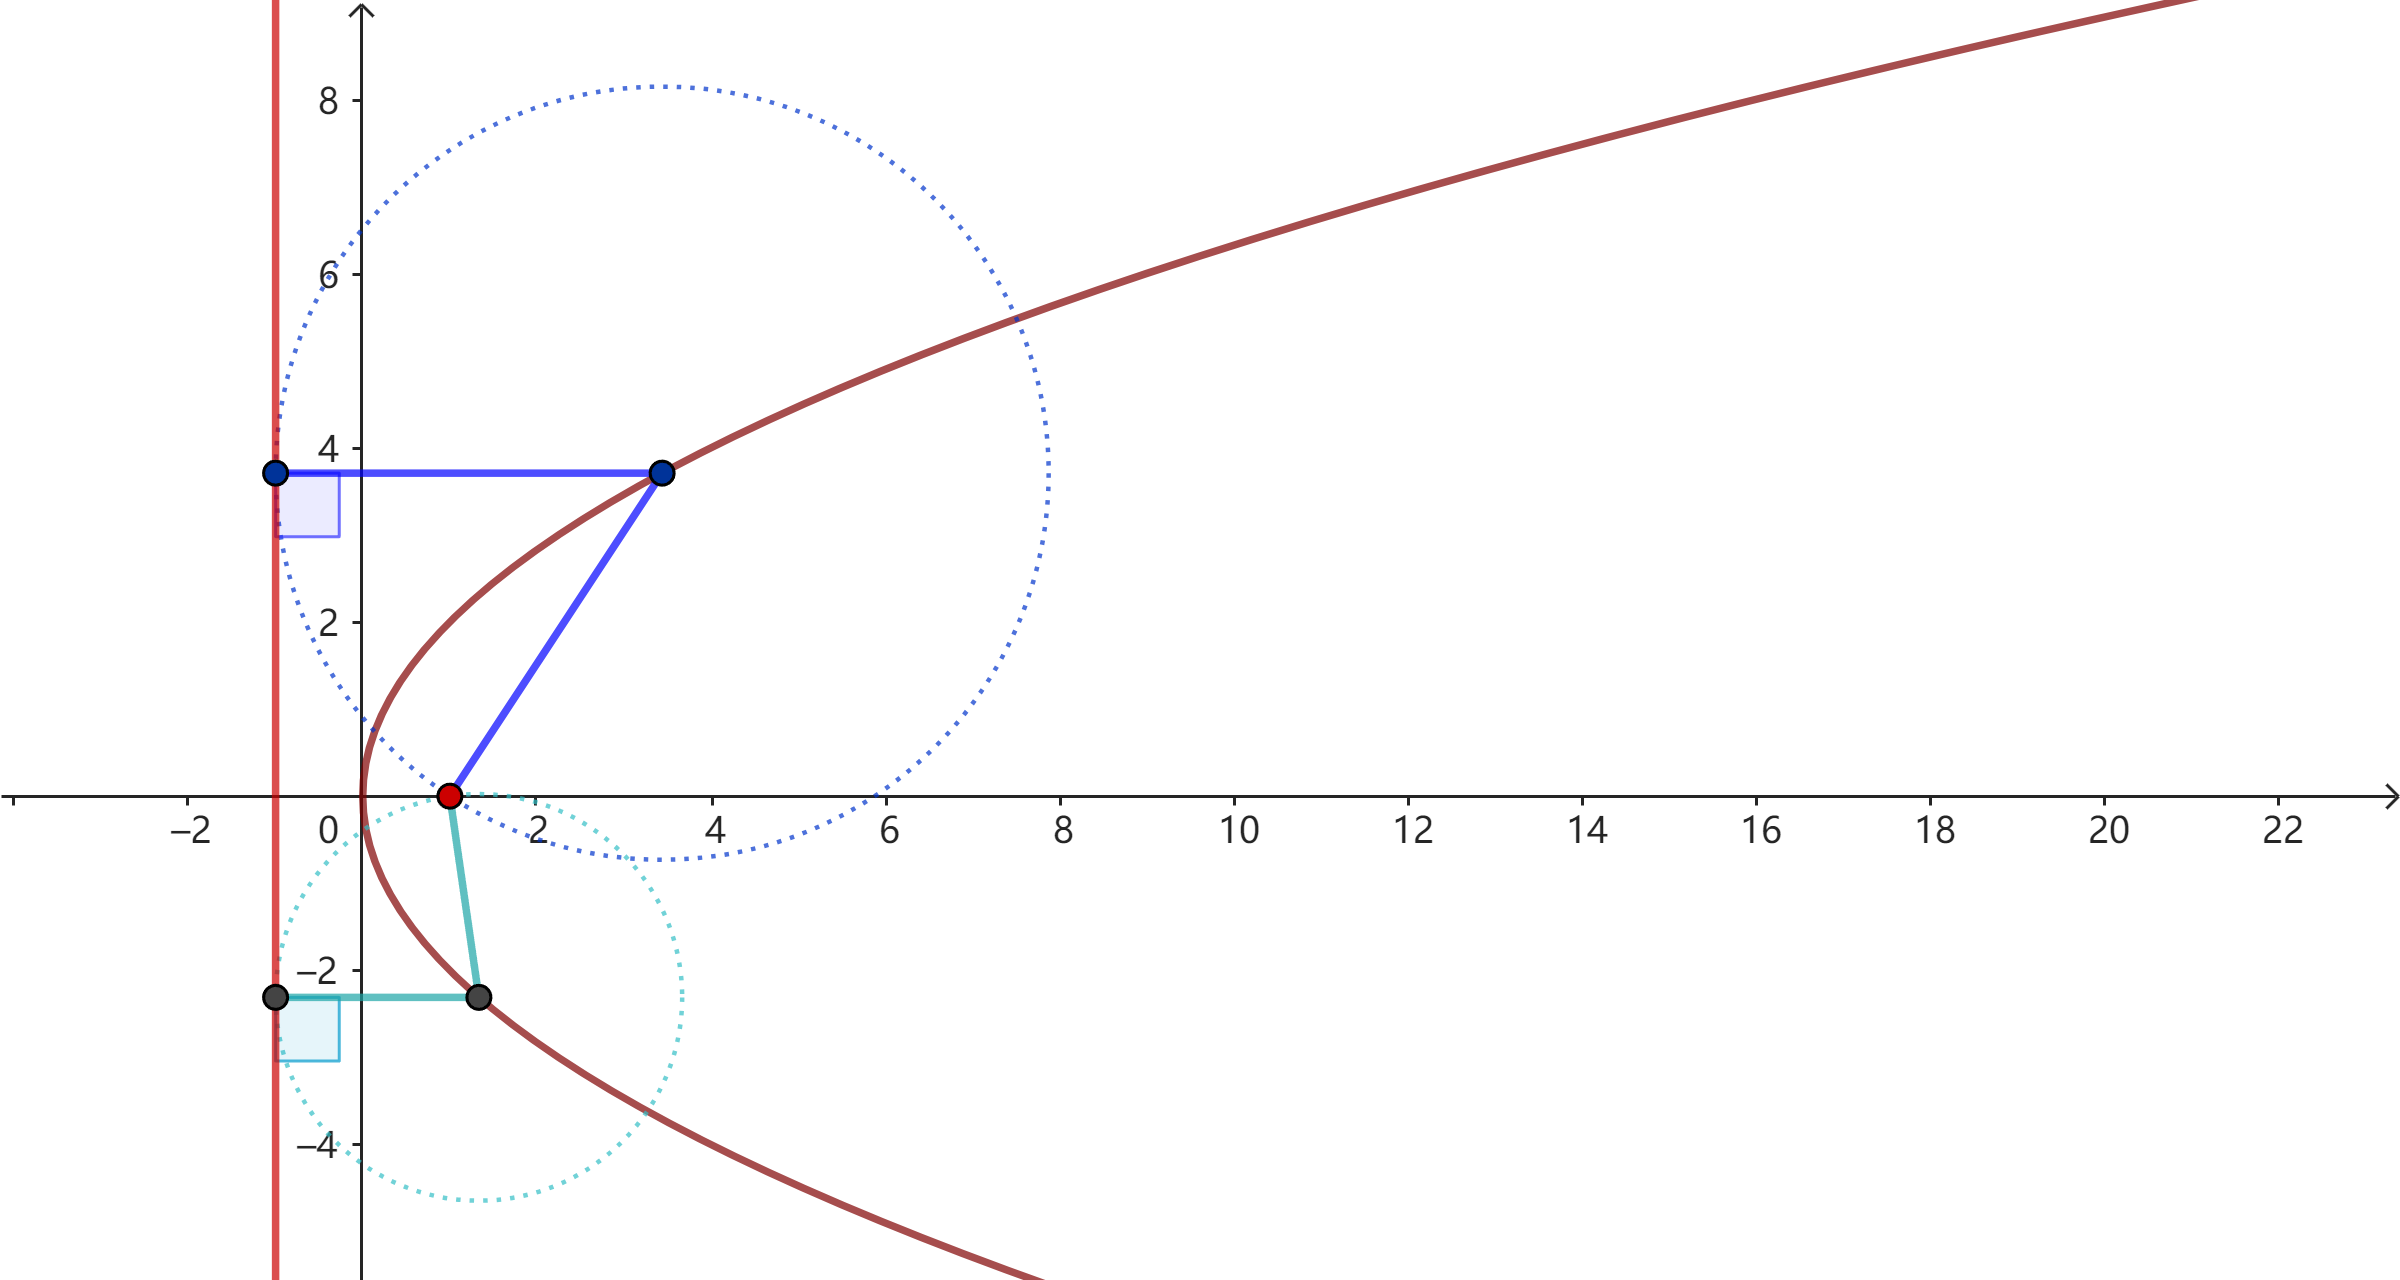
\includegraphics[width=0.8\textwidth]{tu/抛物线第一定义.png}
    \caption*{\texttt{到定点与定直线距离相等的点的轨迹}}
\end{figure}

以上是三类二次曲线的直观定义,也称为它们的\textbf{第一类定义}。

除此以外,我们还可以用另一种直观方式定义二次曲线。

考虑椭圆
$$ \frac{x^2}{a^2} + \frac{y^2}{b^2} = 1.$$
在前面的计算中,我们得到椭圆上一点$P(x,\,\,y)$到焦点$F_2$的距离之和为:
$$ \sqrt{(x - c)^2 + y^2} = \left|a - \frac{cx}{a}\right|.$$
其中$\frac{c}{a} = e < 1$是离心率。于是:
$$  \sqrt{(x - c)^2 + y^2} = e\left|x - \frac{a}{e}\right| . $$
也就是说,$|PF_2|$与$P$到直线$x = \frac{a}{e}$的距离的比值是定值$e$。
反之,如果某点$P:(x,\,\,y)$满足上面的方程,则可以解得:
$$ (x - c)^2 + y^2 = \frac{c^2x^2}{a^2} + a^2 -2cx.$$
于是
$$ \frac{x^2}{a^2} + \frac{y^2}{b^2} = 1.$$
这说明$P$的轨迹是椭圆。这说明椭圆可以定义为$|PF_2|$与$P$到直线$x = \frac{a}{e}$的距离的比值为定值$e<1$的点。

同样,我们也可以定义椭圆为$|PF_1|$与$P$到直线$x = -\frac{a}{e}$的距离的比值为定值$e<1$的点。

我们把以上两直线称为关于相应焦点的\textbf{准线}。椭圆可以定义为到定点和定直线距离之比为定值$e<1$的点。

对于双曲线,我们可以做类似的验证,双曲线也定义为到定点和定直线距离之比为定值的点,只不过定值$e > 1$。

综上,我们可以这样定义三类二次曲线。设有定点$F$、定直线$l$以及正数$e$。
考虑到$F$的距离和$l$的距离之比为$e$的点的轨迹,则:
\begin{itemize}
    \item $e<1$对应椭圆;
    \item $e = 1$对应抛物线;
    \item $e >1$对应双曲线。
\end{itemize}
我们把这种定义称为\textbf{二次曲线的第二类定义}。定义中的直线统一称为\textbf{准线}。

\begin{figure}[h] 
    % \vspace{-4pt}
    \centering
    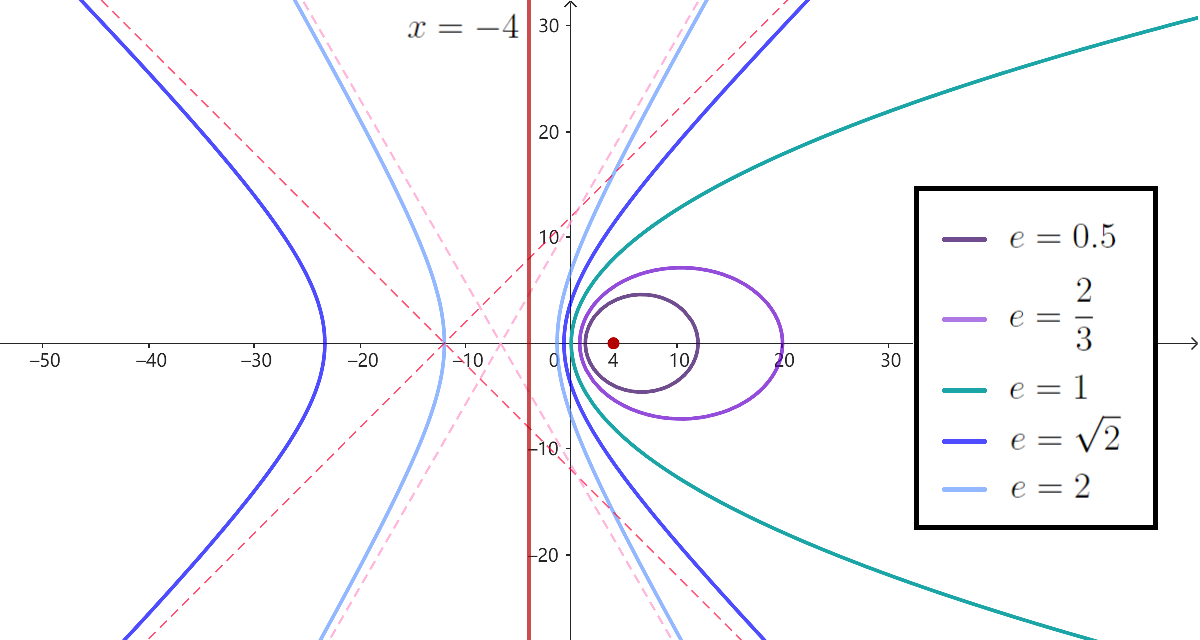
\includegraphics[width=0.8\textwidth]{tu/二次曲线第二定义1.png}
    \caption*{\texttt{到点}$(4,\,\,0)$\texttt{与到直线}$x=-4$\texttt{距离之比为}$e$\texttt{的点的轨迹}}
\end{figure}
以上的定义从平面上的点和直线出发。然而,二次曲线最古老的定义和一种空间形体——圆锥——有关,
因此二次曲线也称为\textbf{圆锥曲线}。从圆锥出发,如何得到二次曲线呢?

考虑配备了直角坐标系$Oxyz$的空间中过原点的直线:
$$ 
\left\{
    \begin{array}{cl}
        z &= kx \qquad (k > 0) \\
        y &= 0
    \end{array}
\right.
$$
以它为母线,绕$z$轴旋转,得到圆锥:
$$ k^2(x^2 + y^2) = z^2. $$

考虑平面$\gamma: \,\,z = ax + b$($a > 0$),设它截圆锥得到一个截面,我们考虑这个截面的边线。

为了研究截面的边线,我们绕$y$轴旋转坐标系,使新$x$轴平行于$\gamma$,新$z$轴方向向量为$\gamma$的法向量。
$xOz$平面上的基变更矩阵为:
$$
\begin{bmatrix}
    \frac{1}{\sqrt{a^2+1}} & -\frac{a}{\sqrt{a^2+1}} \\
    \frac{a}{\sqrt{a^2+1}} & \frac{1}{\sqrt{a^2+1}}
\end{bmatrix}
$$
于是$(x,\,\,y,\,\,z)$在新坐标轴里的坐标$(x',\,\,y',\,\,z')$满足:
$$
\begin{bmatrix}
    x \\ y \\ z
\end{bmatrix}
= 
\begin{bmatrix}
    \frac{x' - az'}{\sqrt{a^2+1}} \\ y' \\ \frac{ax' + z'}{\sqrt{a^2+1}}
\end{bmatrix}
$$
新坐标系中,平面$\gamma$的方程变为$z'=\frac{b}{\sqrt{a^2+1}}$,
而圆锥方程变为:
$$ k^2\frac{(x' - az')^2}{a^2+1} + k^2y^2 = \frac{(ax' + z')^2}{a^2+1} . $$
即:
$$ k^2(a^2+1)y'^2 + (k^2 - a^2)x'^2 - 2az'(1 + k^2)x' = (1 - a^2k^2)z'^2 $$
可以看到方程为二次曲线的方程。由于$y^2$的系数总大于零,$xy$项系数总为零,
$a<k$、$a=k$、$a>k$这三种情形分别对应三类二次曲线。

% 平面截圆锥得到二次曲线例图

直观来说,用平面截圆锥,就能得到二次曲线。二次曲线的类型取决于圆锥母线斜率和截面斜率的关系。
如果母线较陡($a<k$),则截面边线为椭圆;反之截面边线为双曲线。若两者斜率一样,则截面边线为抛物线。

\begin{sk}
    \mbox{} \\
    \indent 1. 
\end{sk}

\begin{xt}
    \mbox{} \\
    \indent 1. 
    
\end{xt}

\section{曲线与函数}

给定平面的曲线,比如椭圆的方程:
$$ \frac{x^2}{a^2} + \frac{y^2}{b^2} = 1,$$
如何研究它的性质呢?

如果曲线是函数的图像,我们可以通过研究微变率,分析它的增减、凹凸性质,可以将它在局部展开,近似为整式函数。
对于一般的曲线,我们也希望能将它转化为函数图像曲线。

曲线无法视为函数的图像,往往是因为多值,即同一个$x$值对应了多个$y$值。
我们可以只取曲线的一部分,将它视为函数的曲线。

具体来说,设曲线$\gamma$的方程为:
$$ F(x, \,\, y) = 0. $$
其中$F$是关于坐标$x$和$y$的多元函数。曲线$\gamma$就是满足方程$F$的点$(x,\,\,y)$的集合。

如果对于某些$x$的值,$F(x, \,\,y) = 0$有唯一解,就是说约束条件$F$将其对应到唯一的$y$。
这时,我们可以认为$y$是关于$x$的函数。这样的函数,称为由$F$确定的\textbf{隐函数}。

\begin{wrapfigure}[10]{r}{0.52\textwidth} %this figure will be at the right
    \vspace{-30pt}
    \flushright
    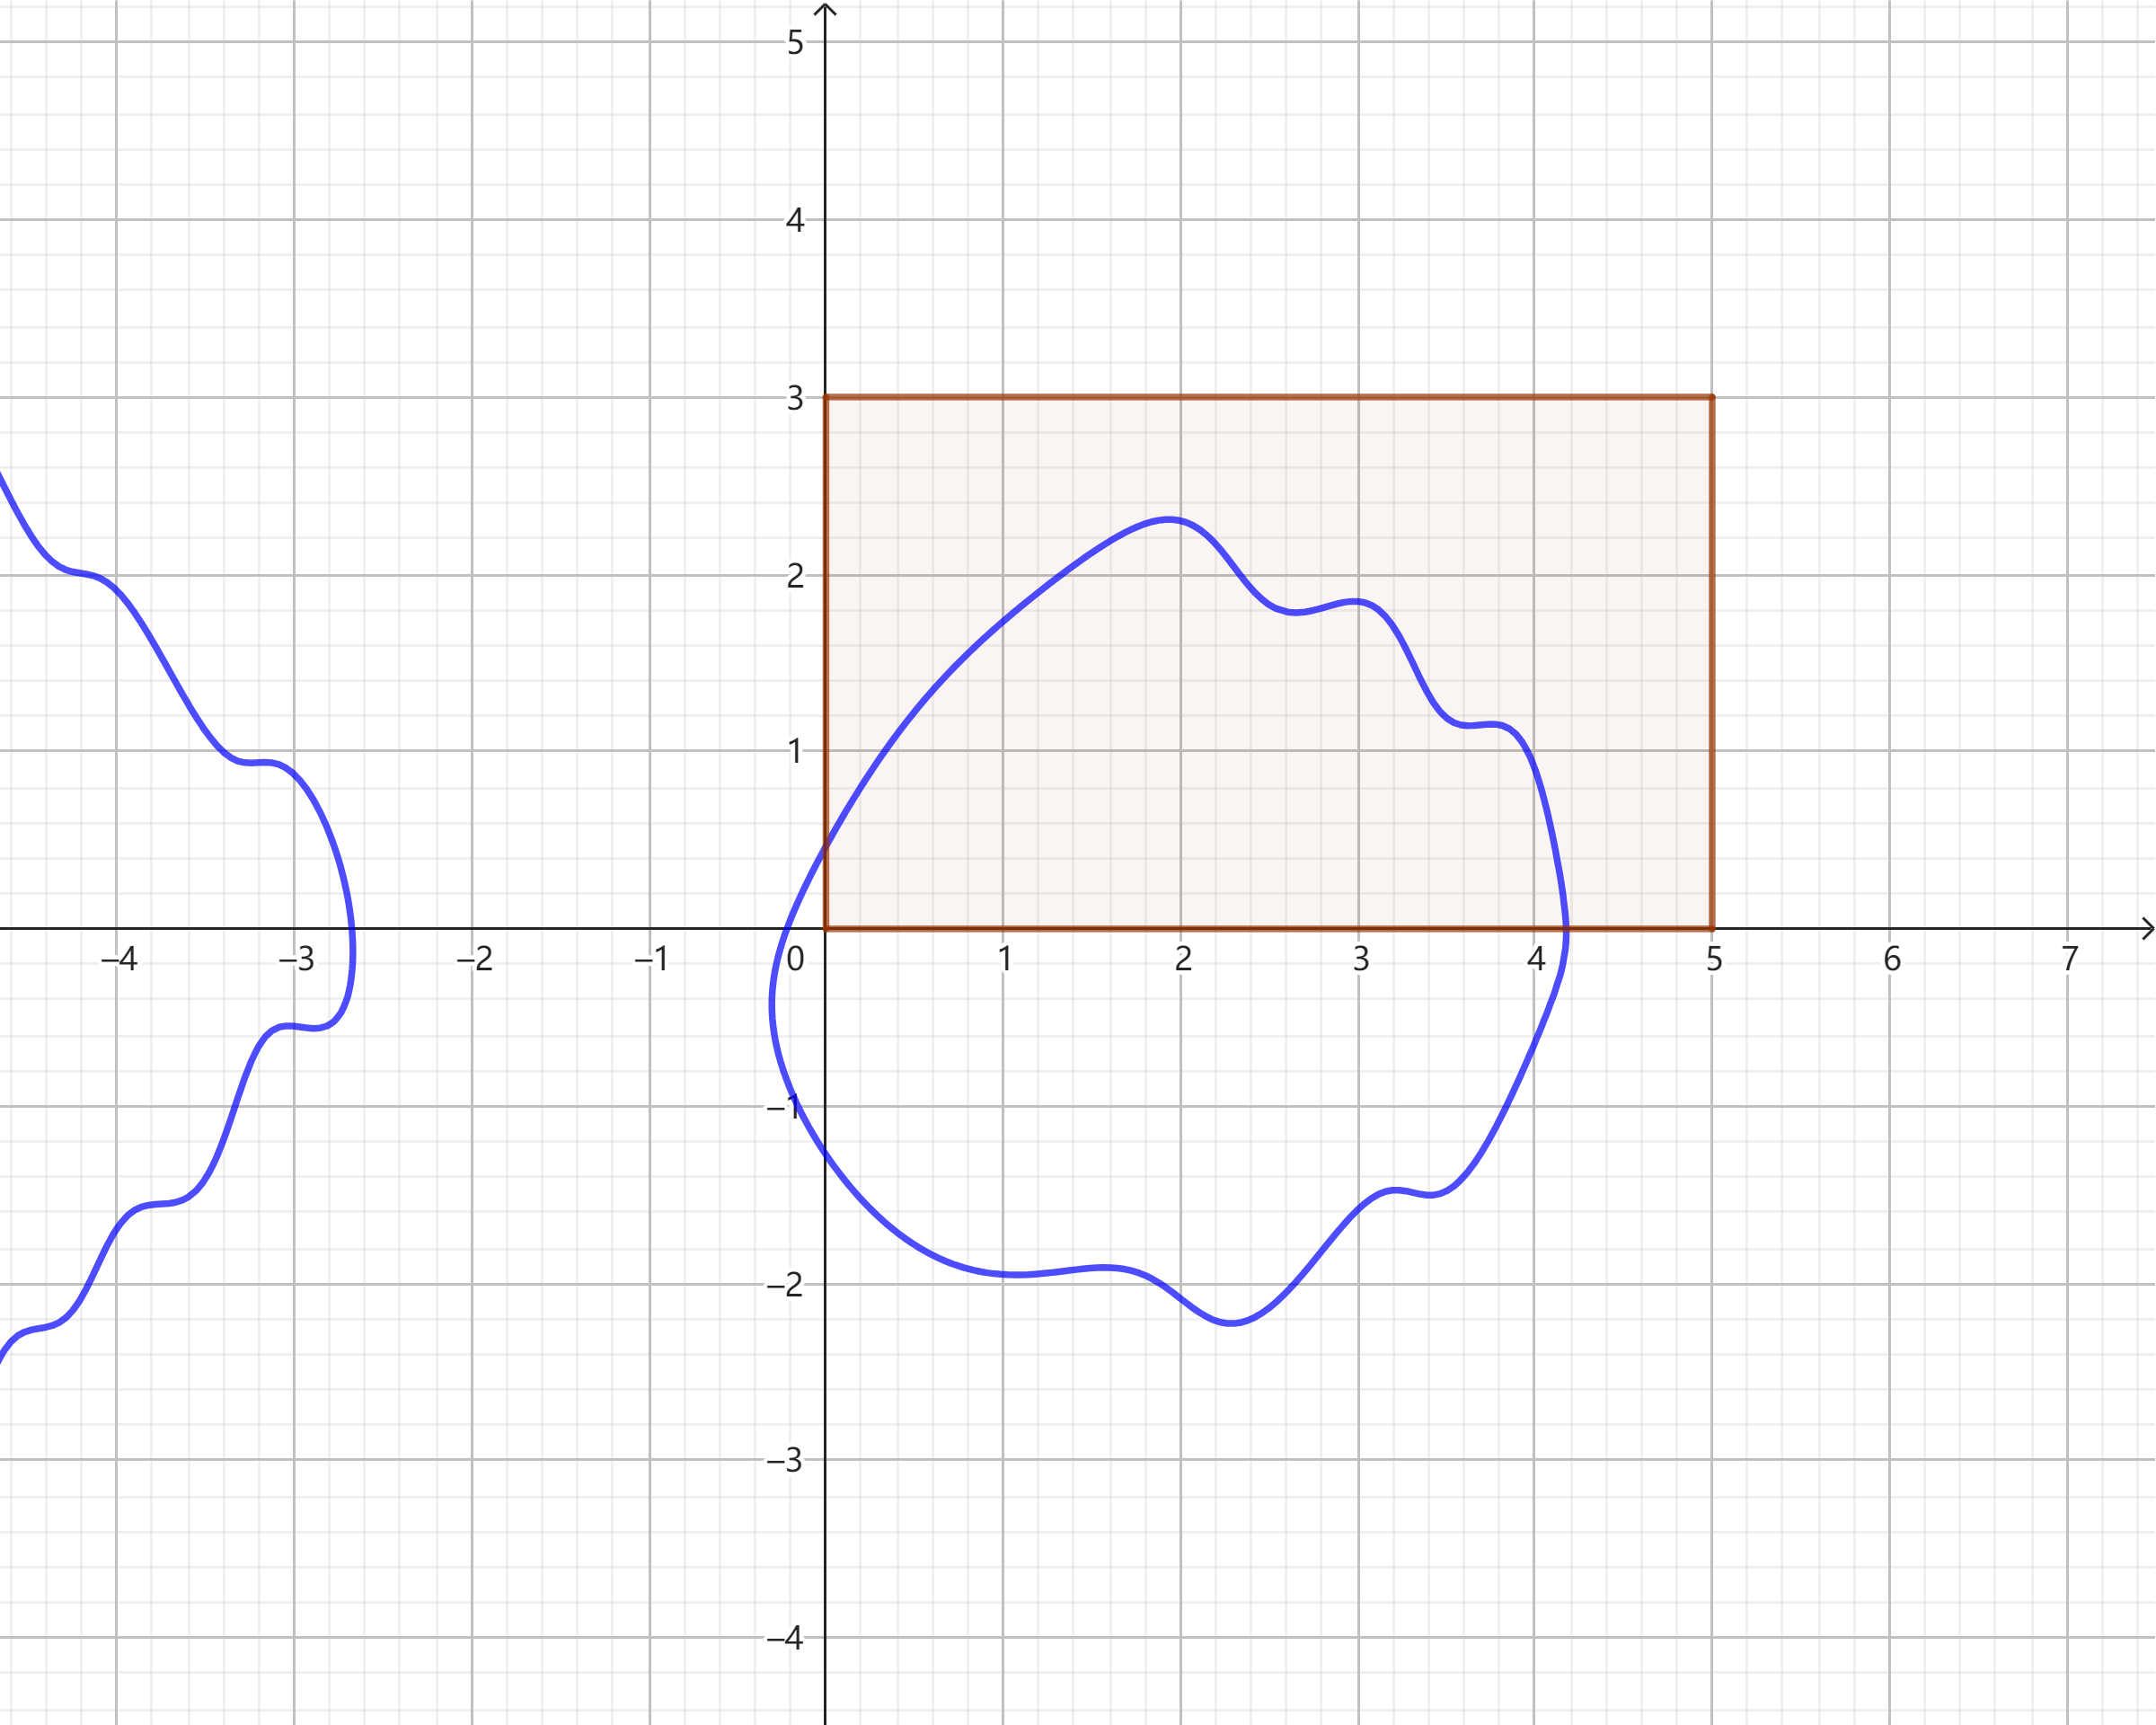
\includegraphics[width=0.5\textwidth]{tu/复杂平面曲线.png}
    \caption*{\texttt{取曲线的一部分,看作函数的曲线}}
\end{wrapfigure}

之所以称为隐函数,是因为我们并不能自动获得隐函数的表达式。
换句话说,我们并不一定知道怎样用$x$表示$y$。我们只知道,
对于$x$来说,$F(x, \,\,y) = 0$有唯一解。这个唯一解就是隐函数的值。

一般来说,使得$F(x, \,\,y) = 0$有唯一解的$x$不一定存在。于是,我们指定平面的子集,
使得$F(x, \,\,y) = 0$在子集中有唯一解。这样就可以确定$y$是关于$x$的隐函数。

以上面给出方程的椭圆为例子。我们知道,椭圆关于$x$轴对称,因此,对每个$x$,都有两个$y$值满足方程,它们互为相反数。
不过,如果只看上半平面,$x$和$y$之间可以有函数关系:
$$ \forall -a\leqslant x \leqslant a, \,\,\, y = b\sqrt{1 - \frac{x^2}{a^2}}= \frac{b}{a}\sqrt{a^2 - x^2}. $$
这就是由$F$确定的隐函数。

综上,对于无法整体视为函数图像的曲线,我们可以通过把平面拆分为子集的方法,把曲线的一部分视为函数图像。
这样的函数称为由曲线方程确定的隐函数。通过研究隐函数,我们可以讨论曲线的性质。

以椭圆为例。通过截取上半平面,我们得到了椭圆上半部分的隐函数
$$ f: x\mapsto y = \frac{b}{a}\sqrt{a^2 - x^2}, \quad x \in [-a, a].  $$
对$f$求微变可得:
$$ \partial f(x) = -\frac{bx}{a}(a^2 - x^2)^{-\frac{1}{2}}$$
微变函数在区间$(-a,0)$上严格单调递增,在$(0,a)$上严格单调递减。隐函数$f$在$0$处取得最大值。
曲线在$(x_0,\,\, y_0)$处的切线为:
\begin{align*}
    y &= f(x_0) + \partial f(x_0)(x - x_0) \\
    &= y_0 -\frac{bx_0}{a\sqrt{a^2 - x_0^2}}(x - x_0) \\
    &= y_0 - \frac{b^2x_0(x - x_0)}{a^2y_0} \\
    &= y_0 - \frac{a^2y_0^2 + b^2x_0^2 - b^2x_0x}{a^2y_0} \\
\end{align*}
由于
$$ \frac{x_0^2}{a^2} + \frac{y_0^2}{b^2} = 1,$$
上式变为
$$ a^2y_0y +  b^2x_0x = a^2b^2. $$
即:
$$ \frac{x_0x}{a^2} + \frac{y_0y}{b^2} = 1.$$
这就是椭圆的切线方程。

对$f$求二次微变可得:
$$ \partial^2 f(x) = -\frac{ab}{(a^2 - x^2)^{\frac{3}{2}} }.$$
$\partial^2 f$在区间$(-a,a)$上总小于零,这说明曲线总是上凸的。


\chapter{参变曲线}

\section{向量函数}

如果曲线不是由方程确定,而是由参变映射确定,我们需要研究的就是把实数(参数)对应到向量的映射。
这种映射也叫做\textbf{实变向量函数}。

实变向量函数和实函数的出发集都是实数域。不同在于实函数将实数自变量映射为实数,而向量函数将实数自变量映射为向量。

参变映射通常用各个坐标的函数表示。比如直线可以用以下的参变映射表示:
\begin{align*}
    f: \mathbb{R} &\rightarrow \mathbb{R}^2 \\
    t\quad &\mapsto\left\{
        \begin{array}[]{rl}
            x(t) &= x_0 + t \\
            y(t) &= y_0 + kt \\
        \end{array}
    \right.
\end{align*}
$f$是关于实数$t$的实变向量函数,而其中$x$、$y$坐标分别是$t$的函数。
它表示经过$(x_0,\,\, y_0)$,斜率为$k$的直线。

而圆可以用以下的参变映射表示:
\begin{align*}
    f: [0,2\pi] &\rightarrow \mathbb{R}^2 \\
    t\quad &\mapsto\left\{
        \begin{array}[]{rl}
            x(t) &= x_C + r\cos{t} \\
            y(t) &= y_C + r\sin{t} \\
        \end{array}
    \right.
\end{align*}
其中自变量$t$在闭区间$[0,2\pi]$上取值。它表示以$(x_C,\,\, y_C)$为圆心,$r$为半径的圆。

% 二次曲线的参变形式:椭圆、双曲线、抛物线
除了圆以外,其他的二次曲线也能用类似的参变映射表示。比如,标准的椭圆可以用以下方式表示:
\begin{align*}
    f: [0,2\pi] &\rightarrow \mathbb{R}^2 \\
    t\quad &\mapsto\left\{
        \begin{array}[]{rl}
            x(t) &= a\cos{t} \\
            y(t) &= b\sin{t} \\
        \end{array}
    \right.
\end{align*}

不难验证,对定义域内任意$t$,总有:
\begin{align*}
    \frac{x^2(t)}{a^2} + \frac{y^2(t)}{b^2} &= \cos^2{t} + \sin^2{t} = 1.
\end{align*}

反之,设$P:(x_P,\,\,y_P)$是椭圆上的点,则
\begin{align*}
    \frac{x_P^2}{a^2} + \frac{y_P^2}{b^2} &= 1\\
   x_P^2 + \left(\frac{a}{b}y_P\right)^2 & = a^2 \\
\end{align*}
这说明点$\displaystyle P': \left(x_P,\,\,\frac{a}{b}y_P\right)$是圆
$$ x^2 + y^2 = a^2$$
上的点,可以表示为$(a\cos{\theta},\,\,a\sin{\theta})$,其中$\theta$是$x$轴到$OP'$的转角。
于是$P$可以表示为$(a\cos{\theta},\,\,b\sin{\theta})$。

同理可以验证,标准的双曲线可以用
\begin{align*}
    f^{\pm}: \mathbb{R} &\rightarrow \mathbb{R}^2 \\
    t\quad &\mapsto\left\{
        \begin{array}[]{rl}
            x(t) &= \pm\frac{a}{2}(e^t + e^{-t}) \\
            y(t) &= \frac{b}{2}(e^t - e^{-t}) \\
        \end{array}
    \right.
\end{align*}
或
\begin{align*}
    f^{\pm}: \mathbb{R} &\rightarrow \mathbb{R}^2 \\
    t\quad &\mapsto\left\{
        \begin{array}[]{rl}
            x(t) &= \frac{a}{2}(e^t - e^{-t}) \\
            y(t) &= \pm\frac{b}{2}(e^t + e^{-t}) \\
        \end{array}
    \right.
\end{align*}
来表示,分别对应左右支和上下支的双曲线。其中$f^+$和$f^-$分别对应双曲线的一支。

为了表述方便,我们可以引入以下两个函数:
\begin{align*}
    \sinh: \mathbb{R} &\rightarrow \quad \mathbb{R} \\
    t\; &\mapsto \frac{e^t - e^{-t}}{2} 
\end{align*}
和
\begin{align*}
    \cosh: \mathbb{R} &\rightarrow \quad \mathbb{R} \\
    t\; &\mapsto \frac{e^t + e^{-t}}{2} 
\end{align*}

这样,双曲线的参数方程可以写为:
\begin{align*}
    f^{\pm}: \mathbb{R} &\rightarrow \mathbb{R}^2 \\
    t\quad &\mapsto\left\{
        \begin{array}[]{rl}
            x(t) &= \pm a\cosh{t} \\
            y(t) &= b\sinh{t} \\
        \end{array}
    \right.
\end{align*}
或
\begin{align*}
    f^{\pm}: \mathbb{R} &\rightarrow \mathbb{R}^2 \\
    t\quad &\mapsto\left\{
        \begin{array}[]{rl}
            x(t) &= a\sinh{t} \\
            y(t) &= \pm b\cosh{t} \\
        \end{array}
    \right.
\end{align*}

$\sinh$和$\cosh$分别称为\textbf{双曲正弦函数}和\textbf{双曲余弦函数}。

抛物线$y^2 = ax$可以简单地用
\begin{align*}
    f: \mathbb{R} &\rightarrow \mathbb{R}^2 \\
    t\quad &\mapsto\left\{
        \begin{array}[]{rl}
            x(t) &= \frac{t^2}{a} \\
            y(t) &= t \\
        \end{array}
    \right.
\end{align*}
来表示。不过,为了方便地指示抛物线的焦点和准线,一般使用
\begin{align*}
    f: \mathbb{R} &\rightarrow \mathbb{R}^2 \\
    t\quad &\mapsto\left\{
        \begin{array}[]{rl}
            x(t) &= pt^2 \\
            y(t) &= 2pt \\
        \end{array}
    \right.
\end{align*}
来表示抛物线。它对应方程为$y^2 = 4px$的抛物线。其中的系数$p$就是抛物线焦点的横坐标。

\begin{sk}
    \mbox{} \\
    \indent 1. 对比三角函数,双曲正弦、余弦函数有什么类似的性质?有什么不同?\\
    \indent 2. 如何用参变映射表示一般形式的二次曲线?\\
\end{sk}

\begin{xt}
    \mbox{} \\
    \indent 1. 考虑以下的参变映射:
    \begin{align*}
        f: \mathbb{R} &\rightarrow \mathbb{R}^2 \\
        t\quad &\mapsto\left\{
            \begin{array}[]{rl}
                x(t) &= x_0 + at^2 \\
                y(t) &= y_0 + bt^2 \\
            \end{array}
        \right.
    \end{align*}
    \indent 1.1. 证明:它代表一条直线。\\
    \indent 1.2. $f$和前面定义的直线的参变映射有什么不同?\\
    \indent 2. 以下的参变映射代表怎样的曲线?
    \begin{align*}
        f: \mathbb{R} &\rightarrow \mathbb{R}^2 \\
        t\quad &\mapsto\left\{
            \begin{array}[]{rl}
                x(t) &= x_0 + a\sin{t} \\
                y(t) &= y_0 + b\sin{t} \\
            \end{array}
        \right.
    \end{align*}
    \indent 3. 考虑以下的参变映射:
    \begin{align*}
        f: \left(-\frac{\pi}{2},\frac{\pi}{2}\right) &\rightarrow \mathbb{R}^2 \\
        t\quad &\mapsto\left\{
            \begin{array}[]{rl}
                x(t) &= a\sec{t} \\
                y(t) &= b\tan{t} \\
            \end{array}
        \right.
    \end{align*}
    \indent 其中$\sec$和$\tan$分别是正割、正切函数。\\
    \indent 3.1. 证明:$f$代表一条双曲线。\\
    \indent 3.2. $f$和前面定义的双曲线的参变映射有什么不同?\\
    \indent 4. 考虑以下的参变映射:
    \begin{align*}
        f: [0,\pi] &\rightarrow \mathbb{R}^2 \\
        t\quad &\mapsto\left\{
            \begin{array}[]{rl}
                x(t) &= a\cos{(1.5t)} \\
                y(t) &= b\sin{(1.5t)} \\
            \end{array}
        \right.
    \end{align*}
    \indent 4.1. 参变映射$f$描述了怎样的曲线?\\
    \indent 4.2. $f$描述的曲线是否是闭曲线?如何将它变为闭曲线?\\
    \indent 5. 如何用参变映射$f$表示抛物线$y^2 = 8x$位于$y = -2$和$y = 4$之间的部分,使得$f(0) = f(1)$?\\
    \indent 6. 考虑以下的参变映射:
    \begin{align*}
        f: \mathbb{R} &\rightarrow \mathbb{R}^2 \\
        t\quad &\mapsto\left\{
            \begin{array}[]{rl}
                x(t) &= 2 - t^2 \\
                y(t) &= t^3 - 1\\
            \end{array}
        \right.
    \end{align*}
    \indent 6.1. 参变映射$f$描述的曲线满足怎样的方程?\\
    \indent 6.2. 该曲线是否有对称中心?是否有对称轴?
\end{xt}

\section{参变曲线的性质}
% 连续和可微
对于实函数,我们建立了连续和微变的概念,可以用来分析函数曲线的性质。
对于向量函数,我们也希望能建立类似的概念,以分析曲线的性质。

连续和微变的概念建立在极限之上。比如,给定函数$f$,$f$在一点$a$连续的定义是:
$$ f (a) = \lian{x\to a} f(x).$$
对于向量函数$g$,我们也想类似定义它在一点的微变。

上式中的极限是这样定义的:
对任意$r>0$,都有$d>0$,使得只要$|x - a| < d$($x$和$a$距离足够小),就有
$$\left|f(x) - f(a)\right| < r,$$
即$f(x)$和$f(a)$距离也足够小。其中我们用绝对值函数来表示自变量和应变量的距离。

对于向量函数,自变量是实数,我们可以继续用绝对值表示自变量的距离,不过,对于应变量,我们需要用另外的方法表示距离。
讨论平面向量,我们一般用经典距离,即两点的坐标差的平方和:
$$ \left\| (x_1, y_1) - (x_2, y_2)\right\| = \sqrt{(x_1 - x_2)^2 + (y_1 - y_2)^2}. $$
除了经典距离,也可以用其他距离,比如坐标差的绝对值之和:
$$ \left\| (x_1, y_1) - (x_2, y_2)\right\| = |x_1 - x_2| + |y_1 - y_2|,$$
或坐标差的最大值:
$$ \left\| (x_1, y_1) - (x_2, y_2)\right\| = |x_1 - x_2| \vee |y_1 - y_2|. $$
这三种距离是讨论平面向量的距离时最常见的,分别称为\textbf{二次距离}($\ell^2$)、\textbf{一次距离}($\ell^1$)和\textbf{绝对距离}($\ell^{\infty}$),对应的距离符号为:
\begin{align*}
    \left\| (x_1, y_1) - (x_2, y_2)\right\|_2 &= \sqrt{(x_1 - x_2)^2 + (y_1 - y_2)^2} \\
    \left\| (x_1, y_1) - (x_2, y_2)\right\|_1 &= |x_1 - x_2| + |y_1 - y_2| \\
    \left\| (x_1, y_1) - (x_2, y_2)\right\|_\infty &= |x_1 - x_2| \vee |y_1 - y_2|
\end{align*}
使用以上距离之一,就可以定义向量函数的连续性质。比如:
对任意$r>0$,都有$d>0$,使得只要$|x - a| < d$,就有
$$\left\|f(x) - f(a)\right\|_2 < r.$$

按照向量距离的定义,我们可以证明:
\begin{tm}
    \textbf{参变映射的局部性质}\\
    \begin{itemize}
        \item 参变映射$t\mapsto (x(t),\,\, y(t))$在$t_0$处极限为$(x_0,\,\,y_0)$,当且仅当函数$x$和$y$在$t_0$处极限为$x_0$和$y_0$。
        \item 参变映射$t\mapsto (x(t),\,\, y(t))$在$t_0$处连续,当且仅当函数$x$和$y$都在$t_0$处连续。
        \item 参变映射$t\mapsto (x(t),\,\, y(t))$在$t_0$处可微,当且仅当函数$x$和$y$都在$t_0$处可微。这时微变率为$(\partial x(t_0),\,\,\partial y(t_0))$。
    \end{itemize}
\end{tm}

举例来说,圆的参变映射中,函数$x$和$y$都连续且可微,所以参变映射$f$也连续且可微。$f$在$t_0$处的微变是:
\begin{align*}
    \partial f(t_0) &= (\partial x(t_0),\,\,\partial y(t_0)) \\
    &= (-r\sin{t_0},\,\, r\cos{t_0}).
\end{align*}
直观来说,这表示圆在点$(\cos{t_0},\,\,\sin{t_0})$处的切线方向可以用向量$(-r\sin{t_0},\,\, r\cos{t_0})$描述,
即切线垂直于点到圆心的线段。向量$(-r\sin{t_0},\,\, r\cos{t_0})$称为圆在$t_0$处的\textbf{切向量}。

直观上,切向量就是曲线在一点切线的方向。曲线在$A$点的切线,可以理解为曲线上另一点$B$足够接近$A$时,直线$AB$的“极限”。
我们认为,对于足够“好”的曲线,只要$B$足够接近$A$,直线$AB$就会趋于一条特定的直线,即曲线在该点的切线。
切线与$B$无关,仅与曲线在$A$点的局部性质有关。

如果曲线的参变映射在$t_0$时位于点$A:(x(t_0),\,\, y(t_0))$,
那么当另一点$B:(x(t),\,\, y(t))$趋于$A$时,直线$AB$的方向为:
$$ \vv{AB} = (x(t) - x(t_0),\,\, y(t) - y(t_0)). $$
如果曲线在$t_0$处连续,那么$t$趋于$t_0$时,$x(t) - x(t_0)$和$y(t) - y(t_0)$都趋于$0$。
不过,如果微变率$(\partial x(t_0),\,\,\partial y(t_0))$是非零向量,那么我们可以把$\vv{AB}$“按比例放大”,即考虑:
$$ \left(\frac{x(t) - x(t_0)}{t - t_0},\,\, \frac{y(t) - y(t_0)}{t - t_0}\right).$$
它的$x$、$y$分量分别对应$x$、$y$函数在$t_0$的变率。
于是,$t$趋于$t_0$时,它趋于$(\partial x(t_0),\,\,\partial y(t_0))$。由于后者是非零向量,它就是曲线在该点的切线的方向。

如果$(\partial x(t_0),\,\,\partial y(t_0))$是零向量,怎么办呢?$x$、$y$函数在该处的微变率都是$0$,
这说明曲线在$t_0$处“停下来了”。我们称它为曲线的\textbf{驻点}。这时,仅仅研究切向量就不够了。

为了进一步研究曲线的局部性质,我们需要把$\vv{AB}$更强力地“按比例放大”,比如让$\vv{AB}$除以$t - t_0$的平方、立方等等。
换句话说,我们可以把$x$、$y$函数在该处做局部展开,通过比较两者的局部行为,确定曲线的局部性质。

具体来说,对足够光滑的曲线,比如$x$、$y$函数都是$n$次连续可微的曲线,我们考虑它们的局部展开:
\begin{align*}
    x(t) &= x(t_0) + \sum_{k=1}^n \frac{\partial^k x (t_0)}{k!}(t - t_0)^k + \olim{(t - t_0)^n} \\
    y(t) &= y(t_0) + \sum_{k=1}^n \frac{\partial^k y (t_0)}{k!}(t - t_0)^k + \olim{(t - t_0)^n}
\end{align*}
也就是说,在$A$附近的一点$(x(t),\,\, y(t))$可以写成:
$$
\begin{bmatrix}
    x(t) \\ y(t)
\end{bmatrix}
=
\begin{bmatrix}
    x(t_0) \\ y(t_0)
\end{bmatrix}
+
\sum_{k=1}^n \frac{(t - t_0)^k}{k!}
\begin{bmatrix}
    \partial^k x(t_0) \\ \partial^k y(t_0)
\end{bmatrix}
+
\olim{(t - t_0)^n}
$$

对$1\leqslant k\leqslant n$,记$k$次微变率构成的向量为$\mathbf{v}_k = (\partial^k x(t_0) ,\,\, \partial^k y(t_0))$,
则$\mathbf{v}_k$对应$(t - t_0)^k$级别的无穷小。
我们从“低”到“高”逐个考察,遇到的第一个非零向量$\mathbf{v}_p$,就是曲线在$t_0$处的\textbf{切向量}。
从$p+1$开始继续考察,遇到的第一个和$\mathbf{v}_p$不共线的向量:$\mathbf{v}_q$,
就是曲线在$t_0$处的\textbf{次方向向量}。
\begin{align*}
    p &= \mbox{使得}\,\mathbf{v}_k\,\mbox{是非零向量的最小下标}\,k\in\{1,2,\cdots, n\}, \\
    q &= \{p+1,p+2,\cdots, n\}\,\mbox{中使得}\,\mathbf{v}_k\,\mbox{与}\,\mathbf{v}_p\,\mbox{不共线的最小下标}\, k. 
\end{align*}

找到了切向量和次方向向量,我们就可以研究曲线在该处的局部性质了。其他的项要么和切向量共线,要么是两者的高阶无穷小。
因此,当$t$趋于$t_0$时,其他项的性质可以忽略。我们可以把$AB$写成:
$$
\vv{AB} = \begin{bmatrix} x(t) \\ y(t) \end{bmatrix} - \begin{bmatrix} x(t_0) \\ y(t_0) \end{bmatrix}
=
\left(\frac{(t - t_0)^p}{p!} + \olim{(t - t_0)^p}\right)\mathbf{v}_p
+
\frac{(t - t_0)^q}{q!}\mathbf{v}_q
+
\olim{(t - t_0)^q}
$$

把平面原点移到$A$处,基底换为$\mathbf{v}_p$和$\mathbf{v}_q$,
那么,在$t_0$附近,我们需要研究的就是新的参数方程:
\begin{align*}
    u = t - t_0 &\mapsto\left\{
        \begin{array}[]{rl}
            x'(u) &\displaystyle = \frac{u^p}{p!} + \olim{u^p} \\
            y'(u) &\displaystyle = \frac{u^q}{q!} \\
        \end{array}
    \right.
\end{align*}
换句话说,我们要关注的是整式函数$H_k: u\mapsto u^k$的性质。

如果$k$是奇数,那么$H_k$是奇函数,$u$从负变正时,$H_k$也从负变正。直观来说,如果某个分量上的参变映射是$H_k$,
那么曲线在该方向上的投影“穿过”$t_0$点。

如果$k$是偶数,那么$H_k$是偶函数,$u$从负变正时,$H_k$从正变为零,再变为正。直观来说,如果某个分量上的参变映射是$H_k$,
那么曲线在该方向上的投影“抵达”$t_0$点,然后“折返”。

因此,根据$p,q$的奇偶性质,可以将曲线在$t_0$处的局部性质分为四类:
\begin{enumerate}
    \item $p$是奇数,$q$是偶数。曲线从第二象限进入第一象限,不穿越切线,凹凸性不变,曲线类似$y = x^2$在$0$点附近的图像。
    \item $p$是奇数,$q$是奇数。曲线从第三象限进入第一象限,穿越切线,凹凸性改变,曲线类似$y = x^3$在$0$点附近的图像。$t_0$是曲线的拐点。
    \item $p$是偶数,$q$是奇数。曲线从第四象限进入第一象限,穿越切线,称$t_0$是曲线的\textbf{顺折点}。
    \item $p$是偶数,$q$是偶数。曲线总在第一象限,不穿越切线,称$t_0$是曲线的\textbf{反折点}。
\end{enumerate}

\begin{figure}[h] 
    \centering
    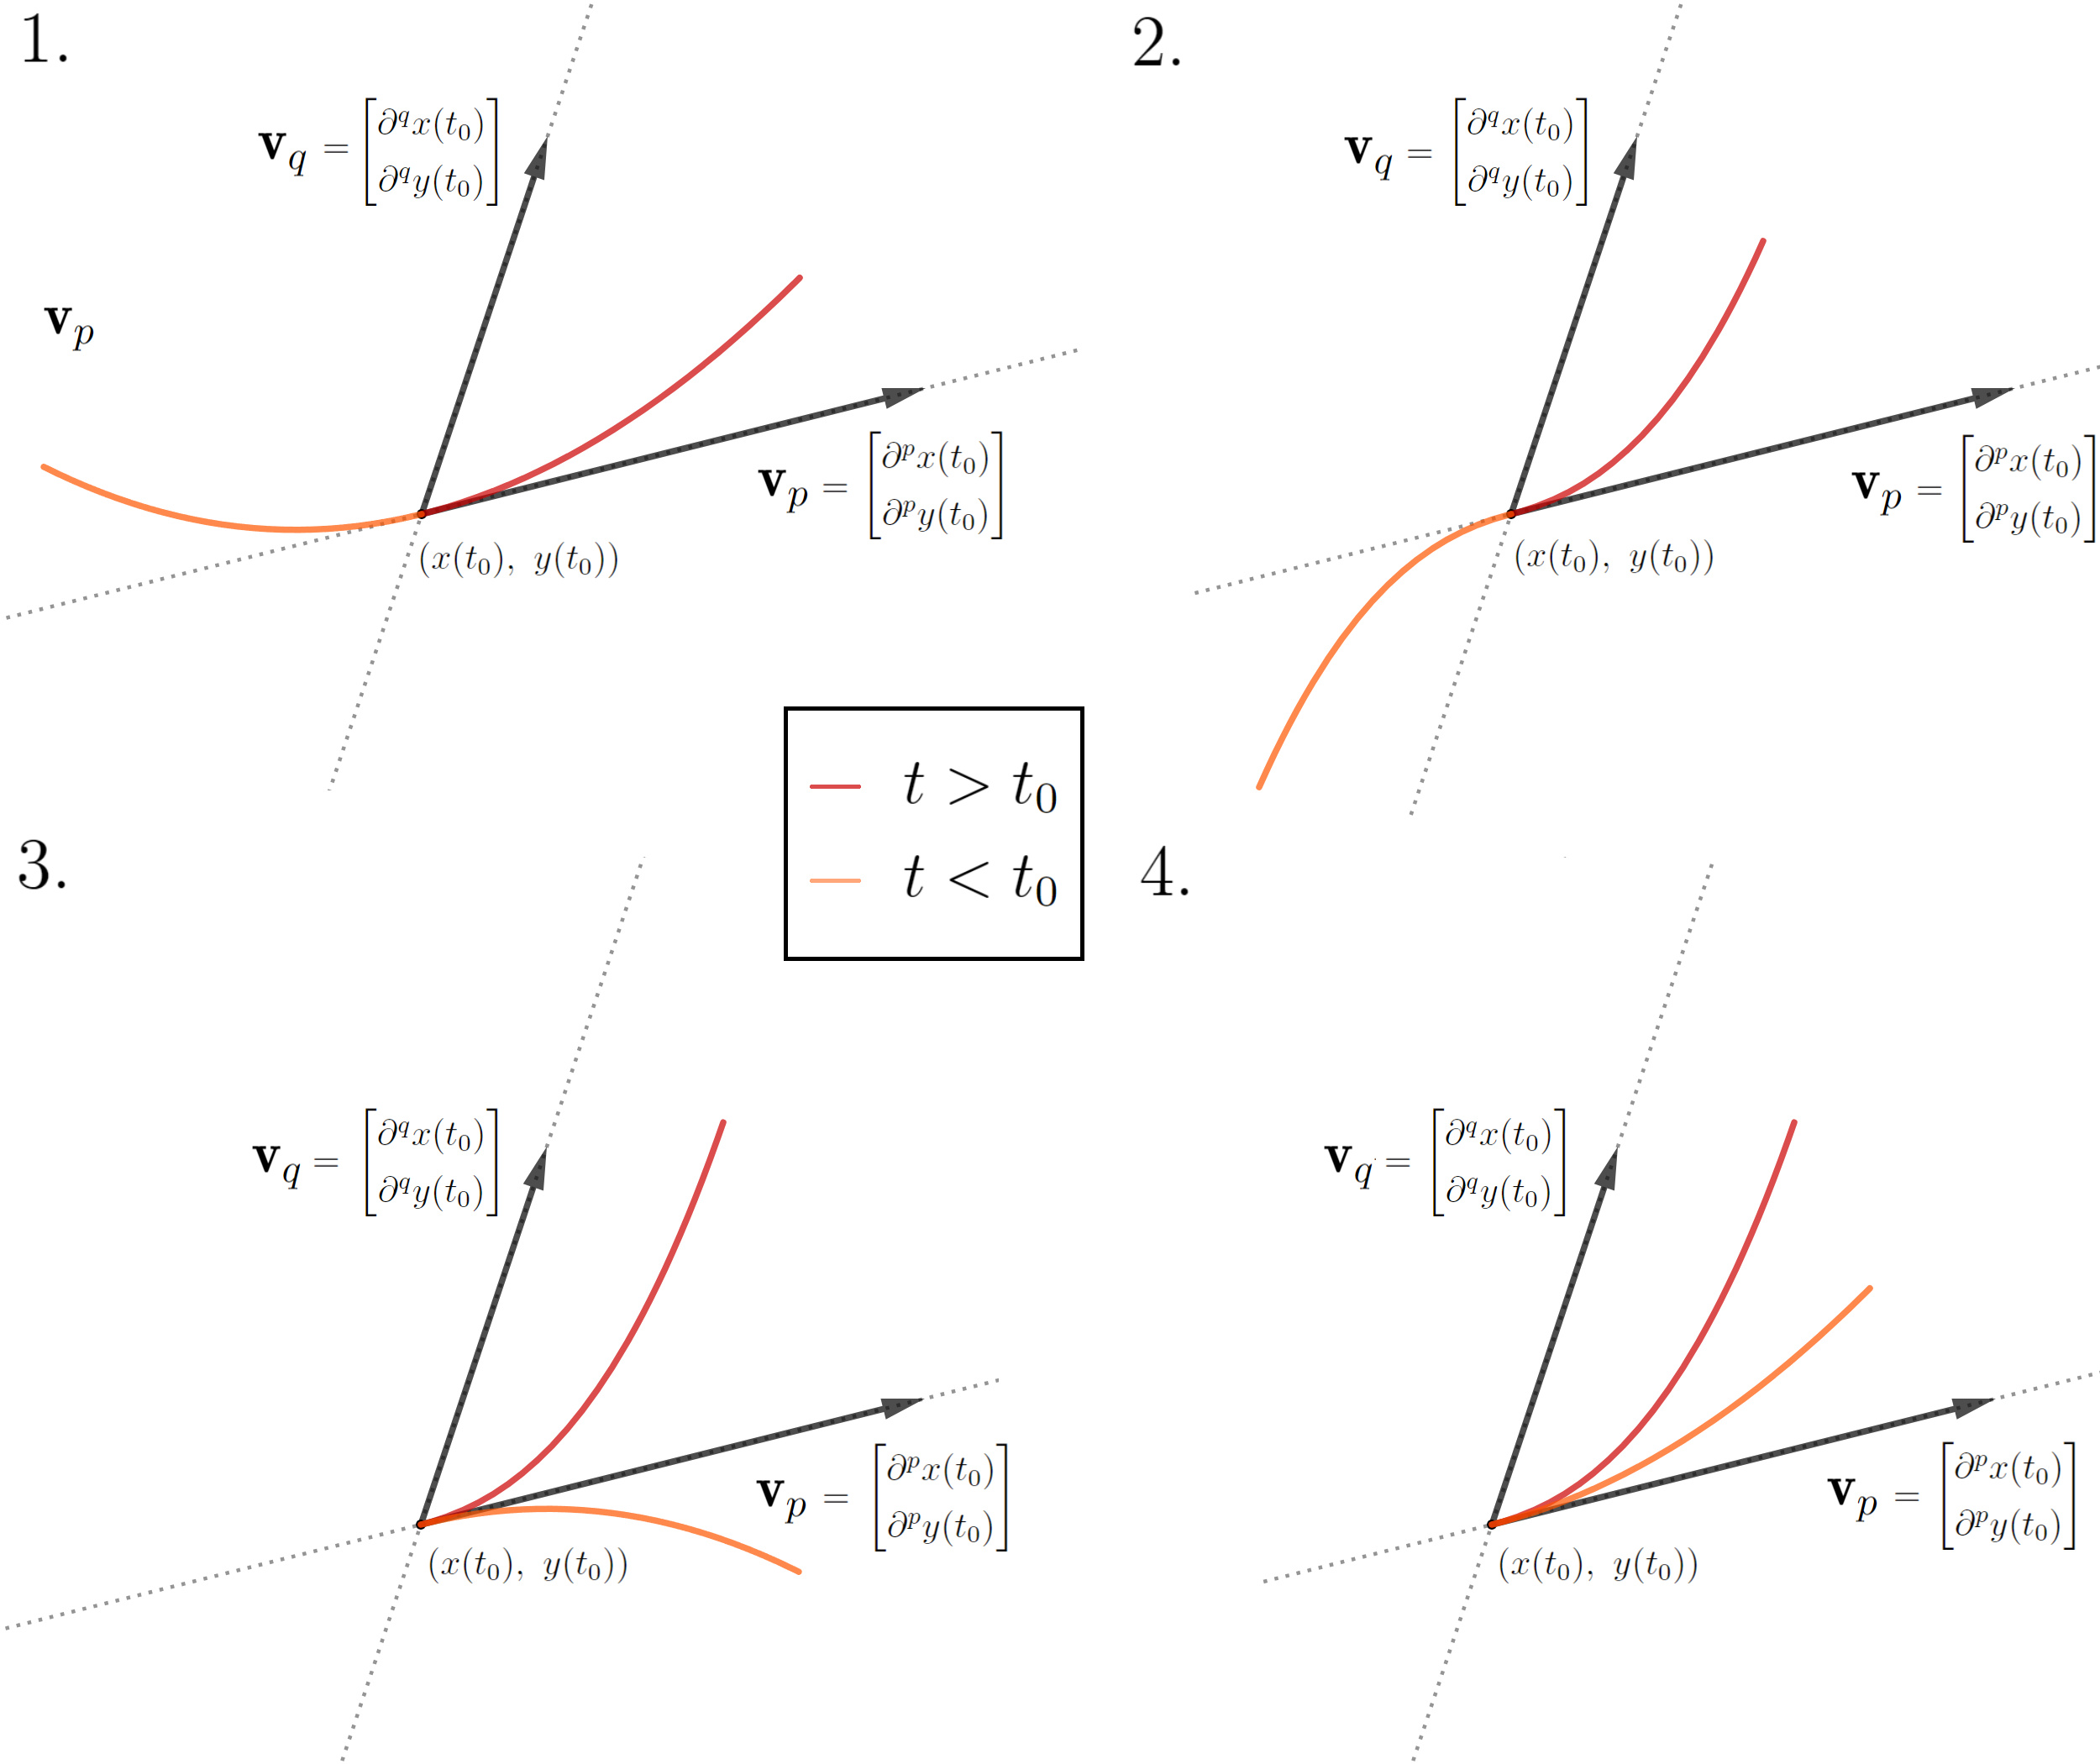
\includegraphics[width=\textwidth]{tu/参数曲线局部展开1.png}
    \caption*{\texttt{参变曲线的局部性质:根据$p,q$奇偶性分为四类情况}}
\end{figure}

参变映射在一点有定义时,可以按以上方法分析。此外,也有参变映射在一点附近有定义,但在该点无定义的情况。
比如$x(t)$或$y(t)$在$t$趋于$t_0$时趋于无穷,或者两者皆然。我们把这种局部情况称为参变曲线\textbf{局部的渐近行为}。

举例来说,考虑参变曲线
\begin{align*}
    f: (0, +\infty) &\rightarrow \mathbb{R}^2 \\
    t\quad &\mapsto\left\{
        \begin{array}[]{rl}
            x(t) &\displaystyle = \frac{1}{t} \\
            y(t) &= t^2\\
        \end{array}
    \right.
\end{align*}
曲线在$t=0$处无定义,但我们需要研究曲线在$t=0$附近的样子。$t>0$趋于$0$时,$x(t)$趋于正无穷,而$y(t)$趋于$0$。
因此,曲线逐渐趋于直线$y = 0$,我们说$y = 0$是曲线在$t=0$处的\textbf{水平渐近线}。

一般来说,如果$t$趋于$t_0$时,$x(t)$趋于正(负)无穷,而$y(t)$趋于某实数$y_0$,那么$y = y_0$是曲线在$t_0$处的水平渐近线。
如果$t$趋于$t_0$时,$y(t)$趋于正(负)无穷,而$x(t)$趋于某实数$x_0$,那么$x = x_0$是曲线在$t_0$处的\textbf{竖直渐近线}。
总之,曲线在局部的渐近行为,表现为无限靠拢渐近线,而具体方向则取决于无穷的正负号。
要注意的是,$t$从$t_0$两侧收敛到$t_0$时,渐近行为要分开讨论。

如果$t$趋于$t_0$时,$x(t)$、$y(t)$都趋于无穷,那么我们需要对这两个无穷大进行比较。
\begin{itemize}
    \item 如果$x(t)$是$y(t)$的高阶无穷大,那么曲线趋于竖直,类似曲线$y = x^2$在$x$趋于无穷时的情况。我们称曲线在$t_0$处\textbf{渐近竖直}。
    \item 如果$y(t)$是$x(t)$的高阶无穷大,那么曲线趋于水平,类似曲线$y^2 = x$在$x$趋于无穷时的情况。我们称曲线在$t_0$处\textbf{渐近水平}。
    \item 如果$\frac{y(t)}{x(t)}$在$t_0$处有极限$a$,那么曲线的渐近行为类似于直线$y = ax$。我们称曲线在$t_0$处\textbf{渐近方向}为向量$(1,\,\,a)$\footnote{或$(-1,\,\,-a)$,取决于$x$、$y$趋于无穷的正负号。下同。}。
    \item 如果曲线有渐近方向$(1, \,\,a)$,则研究$y(t) - ax(t)$。如果它在$t_0$处有极限$b$,那么$y = ax + b$为曲线在$t=0$处的渐近线。如果$y(t) - ax(t)$趋于无穷,那么曲线的渐近行为类似于倾斜的抛物线,我们说曲线在$t_0$处\textbf{抛物渐近}$y = ax$。
\end{itemize}

\begin{et}
    \mbox{} \\
    研究参变曲线:% 例题
    \begin{align*}
        f: (-\infty,0) &\rightarrow \mathbb{R}^2 \\
        t\quad &\mapsto\left\{
            \begin{array}[]{rl}
                x(t) &=2t + t^2 \\
                y(t) &\displaystyle = 2t - \frac{1}{t^2}\\
            \end{array}
        \right.
    \end{align*}
    在$t=-1$附近的性质。
\end{et}

\begin{so}
    参变映射在$t=-1$处的值为$(-1, \,\,-3)$,函数$x$、$y$在该处连续且可微。
    $$
    \left\{
        \begin{array}[]{rl}
            \partial x(t) &=2 + 2t \\
            \partial y(t) &\displaystyle = 2 + \frac{2}{t^3}\\
        \end{array}
    \right.
    $$
    所以
    $$
    \left\{
        \begin{array}[]{rl}
            \partial x(-1) &= 0 \\
            \partial y(-1) & 0\\
        \end{array}
    \right.
    $$
    零向量无法作为切向量,因此继续求二次微变:
    $$
    \left\{
        \begin{array}[]{rl}
            \partial^2 x(t) &=2 \\
            \partial^2 y(t) &\displaystyle = - \frac{6}{t^4}\\
        \end{array}
    \right.
    $$
    因此在$t=-1$处,二次微变向量$\mathbf{v}_2 = (2, \,\,-6)$,可以作为切向量,$p=2$。

    继续考察高次微变。计算可知$t=-1$处的三次微变向量$\mathbf{v}_3 = (0, \,\,-24)$,与$\mathbf{v}_2$不共线。
    于是$q=3$。
    
    我们得到切向量为$(1,\,\,-3)$,次方向向量为$(0,\,\,-1)$。$p=2$为偶数,$q=3$为奇数。
    这说明曲线在$t=-1$处有顺折点。
\end{so}

\begin{figure}[h] 
    % \vspace{-4pt}
    \centering
    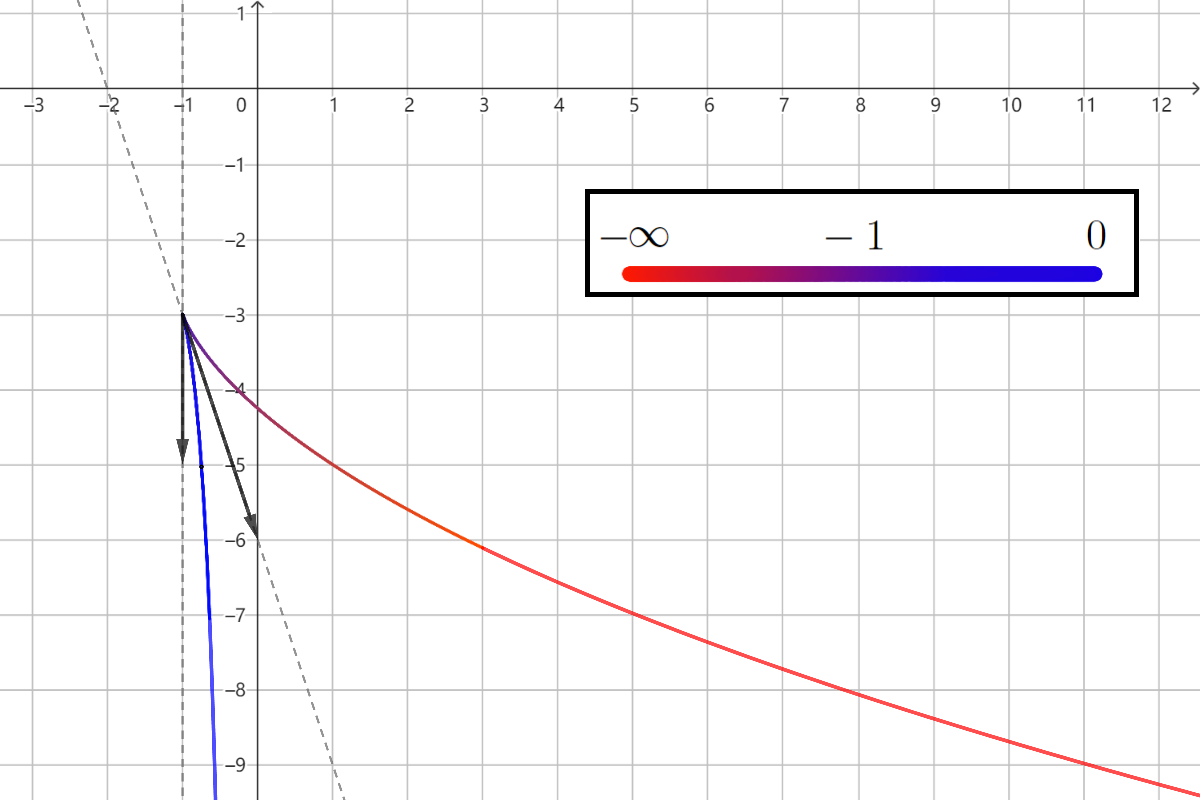
\includegraphics[width=0.8\textwidth]{tu/曲线局部渐近行为01.png}
    \caption*{\texttt{$t$经过$-1$时,曲线在$(-1, \,\,-3)$处停驻并顺折}}
\end{figure}

\begin{et}
    \mbox{} \\
    研究参变曲线:% 例题
    \begin{align*}
        f: (0,+\infty) &\rightarrow \mathbb{R}^2 \\
        t\quad &\mapsto\left\{
            \begin{array}[]{rl}
                x(t) &\displaystyle = t^2 + \frac{2}{t} \\
                y(t) &\displaystyle = t + 3 + \frac{1}{t}\\
            \end{array}
        \right.
    \end{align*}
    在$t=0$附近的性质。
\end{et}

\begin{so}
    当$t$趋于$0^+$时\footnote{指$t>0$且趋于$0$。下同。},$x(t)$和$y(t)$都趋于正无穷。研究两者之比:
    \begin{align*}
        \frac{y(t)}{x(t)} = \frac{t + 3 + \frac{1}{t}}{t^2 + \frac{2}{t}} = \frac{t^2 + 3t + 1}{t^3 + 2}.
    \end{align*}
    因此 
    $$ \lian{t\to 0^+} \frac{y(t)}{x(t)} = \lian{t\to 0^+} \frac{t^2 + 3t + 1}{t^3 + 2} = \frac{1}{2}. $$
    这说明渐近方向为$(2,\,\,1)$。继续研究$y(t) - \frac{1}{2}x(t)$。
    \begin{align*}
        y(t) - \frac{1}{2}x(t) &= t + 3 + \frac{1}{t} - \frac{1}{2}\left(t^2 + \frac{2}{t}\right) \\
        &= t + 3 - \frac{t^2}{2}.
    \end{align*}
    因此
    $$ \lian{t\to 0^+} y(t) - \frac{1}{2}x(t) = \lian{t\to 0^+} t + 3 - \frac{t^2}{2} = 3. $$
    这说明$t$趋于$0^+$时,曲线有渐近线:$y = \frac{1}{2}x + 3$。

    $y(t) - \frac{1}{2}x(t) - 3 = t + \olim{t}$,因此,当$t>0$足够接近$0$的时候,曲线在渐近线上方,与渐近线的距离趋于$0$。
\end{so}

\begin{figure}[h] 
    % \vspace{-4pt}
    \centering
    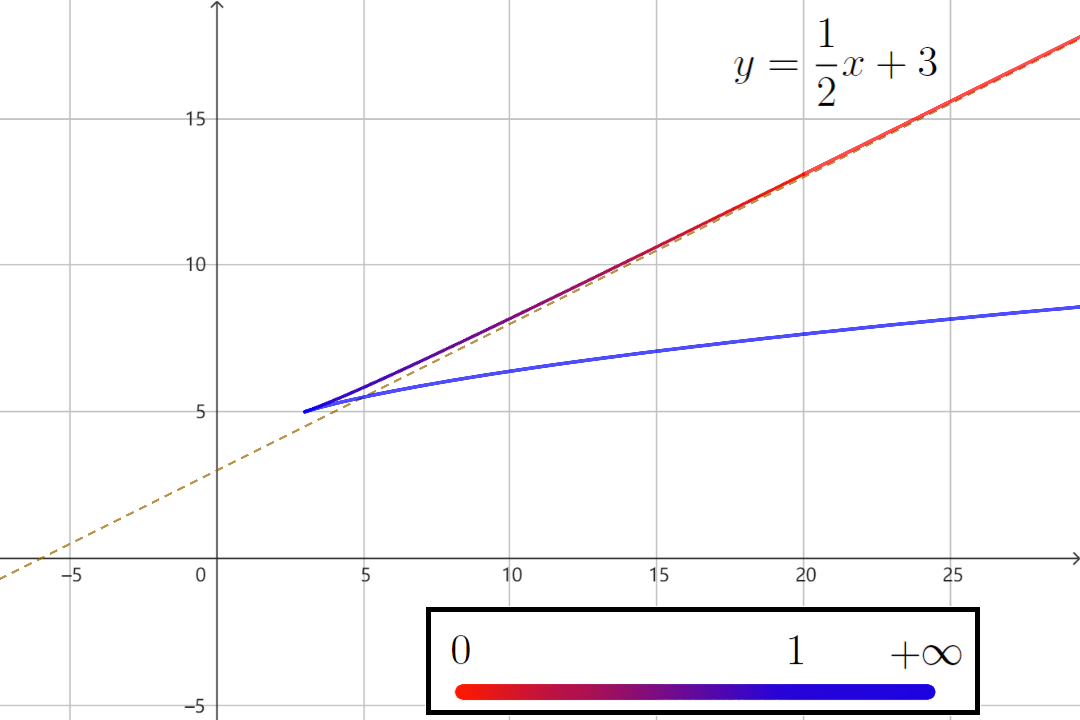
\includegraphics[width=0.8\textwidth]{tu/曲线局部渐近行为02.png}
    \caption*{\texttt{$t$趋于$0^+$时({\color{red}红}),曲线趋于渐近线}}
\end{figure}

\begin{sk}
    \mbox{} \\
    \indent 1. 为什么参变曲线有切向量为零向量的情况,而函数曲线没有这样的情况?\\
    \indent 2. 如果参变量趋于无穷时,参变映射$x$、$y$趋于定值$x_0$、$y_0$,如何研究曲线在$(x_0,\,\,y_0)$附近的性质?\\
    \indent 3. 如果参变量趋于$t_0$时,参变映射$x$或$y$趋于无穷,$x$、$y$的正负号如何影响曲线在局部的渐近行为?分情况讨论。\\
    \indent 4. 能否用关于极坐标的参变映射表示平面曲线?如何研究相关的局部性质?
\end{sk}

\begin{xt}
    \mbox{} \\
    \indent 1. 研究以下参变曲线在$t=0$附近的性质:
    \begin{align*}
        1).\quad f: \mathbb{R} &\rightarrow \mathbb{R}^2 & \quad 2).\quad f: \mathbb{R} &\rightarrow \mathbb{R}^2 \\
        t\quad &\mapsto\left\{
            \begin{array}[]{rl}
                x(t) &= t + 2t^2 - t^3 \\
                y(t) &= t + 2t^2 - t^7 \\
            \end{array}
        \right.
        & \quad 
        t\quad &\mapsto\left\{
            \begin{array}[]{rl}
                x(t) &= t^2 - t \\
                y(t) &= t^2 + t^3 \\
            \end{array}
        \right.
    \end{align*}
    \begin{align*}
        \;\;3).\quad f: \mathbb{R} &\rightarrow \mathbb{R}^2 &  4).\quad f: \mathbb{R} &\rightarrow \mathbb{R}^2 \\
        \;\;t\quad &\mapsto\left\{
            \begin{array}[]{rl}
                x(t) &= t^2 + 3t^3 + t^4 \\
                y(t) &= t^4 - 2t^2 - 6t^3 \\
            \end{array}
        \right.
        & 
        t\quad &\mapsto\left\{
            \begin{array}[]{rl}
                x(t) &= t^2 + 2t^3 \\
                y(t) &= t^3 + t^5 \\
            \end{array}
        \right.
    \end{align*}
    \indent 2. 考虑参变曲线:
    \begin{align*}
        f: [0,+\infty) &\rightarrow \mathbb{R}^2 \\
        t\quad &\mapsto\left\{
            \begin{array}[]{rl}
                x(t) &\displaystyle = \frac{t}{1 + t^4} \\
                y(t) &\displaystyle = \frac{t^3}{1 + t^4} \\
            \end{array}
        \right.
    \end{align*}
    \indent 2.1. 比较$f(t)$和$\displaystyle f\left(\frac{1}{t}\right)$,能得到什么结论?这说明曲线具有什么性质?证明:可以将曲线研究范围缩减到$[0,1]$。\\
    \indent 2.2. 研究$x(t)$和$y(t)$在$[0,1]$上的性质,据此画出曲线的形状。\\
    \indent 3. 考虑参变曲线:
    \begin{align*}
        f: \mathbb{R} &\rightarrow \mathbb{R}^2 \\
        t\quad &\mapsto\left\{
            \begin{array}[]{rl}
                x(t) & = 2\cos{t} - \cos{2t} \\
                y(t) & = 2\sin{t}\, - \sin{2t} \\
            \end{array}
        \right.
    \end{align*}
    \indent 3.1. 证明:随着$t$在$\mathbb{R}$中变化,$f$周期性沿着闭曲线运动。找出最小的周期$T$。\\
    \indent 3.2. 证明:$f$的轨迹关于$x$轴对称。因此,可以将曲线研究范围缩短。给出合适的研究区间。\\
    \indent 3.3. 研究$x(t)$和$y(t)$在该区间上的性质,据此画出曲线的形状。\\
    \indent 4. 研究以下参变曲线在$t=0$附近的性质:
    \begin{align*}
        1).\quad f: \mathbb{R}^+ &\rightarrow \mathbb{R}^2 & \quad 2).\quad f: \mathbb{R}^+ &\rightarrow \mathbb{R}^2 \\
        t\quad &\mapsto\left\{
            \begin{array}[]{rl}
                x(t) &\displaystyle = \frac{1+t^2}{t} \\
                y(t) &\displaystyle = 2 - \frac{1}{t} \\
            \end{array}
        \right.
        & \quad 
        t\quad &\mapsto\left\{
            \begin{array}[]{rl}
                x(t) &\displaystyle = \frac{1+t}{t^2} \\
                y(t) &\displaystyle = \frac{1-2t}{t^2} \\
            \end{array}
        \right.
    \end{align*}
    \begin{align*}
        \;\;3).\quad f: \mathbb{R}^+ &\rightarrow \mathbb{R}^2 &  4).\quad f: \mathbb{R}^+ &\rightarrow \mathbb{R}^2 \\
        \;\;t\quad &\mapsto\left\{
            \begin{array}[]{rl}
                x(t) &\displaystyle = \frac{1+t}{t^2} \\
                y(t) &\displaystyle = 2 - \frac{1}{t} \\
            \end{array}
        \right.
        & 
        t\quad &\mapsto\left\{
            \begin{array}[]{rl}
                x(t) &\displaystyle = 1 - \frac{1+t}{t^2} \\
                y(t) &\displaystyle = 2 - \frac{1}{t^2} \\
            \end{array}
        \right.
    \end{align*}
    \indent 5. 考虑参变曲线:
    \begin{align*}
        f: \mathbb{R}\setminus\{0\} &\rightarrow \mathbb{R}^2 \\
        t\quad &\mapsto\left\{
            \begin{array}[]{rl}
                x(t) &\displaystyle = t + \frac{1}{t} \\
                y(t) &\displaystyle = t + \frac{1}{2t^2} \\
            \end{array}
        \right.
    \end{align*}
    \indent 5.1. 考虑$t$趋于正负无穷时$x(t)$和$y(t)$的变化,说明曲线此时的性质。\\
    \indent 5.2. 考虑$t$趋于$0^+$时$x(t)$和$y(t)$的变化,说明曲线此时的性质。\\
    \indent 5.3. 考虑$t$趋于$0^-$时$x(t)$和$y(t)$的变化,说明曲线此时的性质。\\
    \indent 5.4. 说明$t$趋于$-1$时曲线的局部性质。\\
    \indent 5.5. 说明$t$趋于$1$时曲线的局部性质。\\
    \indent 5.6. 研究$x(t)$和$y(t)$的变化,画出曲线的形状。
\end{xt}


% \section{微变方程和参变曲线}
% % 由微变方程确定的参变曲线

% \begin{sk}
%     \mbox{} \\
% \end{sk}

% \begin{xt}
%     \mbox{} \\
% \end{xt}

\begin{appendix}

\chapter{函数的级数}
\begin{tm}{\textbf{一致收敛保证极限}}
    已知区间$I$上的函数列$\{f_n\}_{n\in\mathbb{N}}$一致收敛到$f$,
    且函数列的每一项$f_n$都在区间的一端$a$点处\footnote{也可以是无穷远处。}有极限$u_n$。
    那么数列$\{u_n\}$收敛到某个数$u$,且$u$是$f$在$a$处的极限。
    $$ \lian{n\to +\infty} \lian{x\to a} f_n(x) = \lian{x\to a} \lian{n\to +\infty} f_n(x). $$
\end{tm}

\begin{tm}{\textbf{一致收敛传递连续性}}
    连续函数的函数列如果一致收敛,极限也是连续函数。
\end{tm}

更进一步有:

\begin{tm}
    如果函数$f$在区间$I$上可微,且微变函数在$I$上连续,就说$f$在$I$上\textbf{一阶光滑}或\textbf{连续可微}。
    如果$f$的前$k$次微变都在$I$上一阶光滑,就说$f$在$I$上$\boldsymbol{k}$\textbf{阶光滑}或$\boldsymbol{k}$\textbf{阶连续可微}。
    如果对任意正整数$k$,$f$在$I$上$k$阶光滑,就说$f$在$I$上\textbf{光滑}。

    已知函数列$\{f_n\}_{n\in\mathbb{N}}$中每一项都在区间$I$上可微,且微变函数连续。
    设函数列逐点收敛到函数$f$,且函数列$\{\partial f_n\}_{n\in\mathbb{N}}$一致收敛到函数$g$,
    那么$\{f_n\}_{n\in\mathbb{N}}$一致收敛到$f$,
    $f$在$I$上可微,且其微变函数$\partial f = g$。

    也就是说,在一定条件下,我们可以交换微变、极限和函数列的极限操作:
    $$ \lian{n\to +\infty} \partial f_n = \partial \lian{n\to +\infty} f_n. $$

    如果函数列$\{f_n\}_{n\in\mathbb{N}}$中每一项都在区间$I$上$k$阶连续可微,简单收敛到某个函数$f$,并且
    \begin{enumerate}
        \item 对任意$1 \leqslant i < k$,函数列$\{\partial^i f_n\}_{n\in\mathbb{N}}$简单收敛到函数$g_i$;
        \item 对任意闭区间$B \subseteq I$,函数列$\{\partial^k f_n\}_{n\in\mathbb{N}}$在$B$上一致收敛到函数$g_k$。
    \end{enumerate}
    那么$f$在$I$上$k$阶连续可微,且其前$k$阶微变函数为$\partial^i f = g_i$($1 \leqslant i\leqslant k$)。
    此外,$\{f_n\}_{n\in\mathbb{N}}$在$I$中任意闭区间一致收敛到$f$。

\end{tm}

\chapter{复数}

\begin{tm}{\textbf{代数基本定理}}
    \mbox{} \\
    次数大于零的复系数整式至少有一个复数根。
\end{tm}

\begin{proof}
    % Oswaldo Rio Branco de Oliveira, The Fundamental Theorem of Algebra: An Elementary and Direct Proof. Math Intelligencer 33, 1–2 (2011). https://doi.org/10.1007/s00283-011-9199-2
    设$P$是次数大于零的整式:
    $$ P(x) = a_0 + a_1 x + \cdots + a_n x^n.$$
    其中$a_0, a_1, \cdots , a_n$是复数,$a_n \neq 0$。
    我们要证明:有复数$z_0\in\mathbb{C}$,使得$P(z_0) = 0$。

    对整式$P$取模:
    $$ |P(x)| = |a_0 + a_1 x + \cdots + a_n x^n|. $$
    根据三角形边长的关系,我们知道:
    $$ |P(x)| \geqslant |a_n| |x|^n - |a_0| - |a_1||x| - \cdots - |a_{n-1}| |x|^{n-1}. $$
    因此,当$|x|$趋于正无穷时,$|P(x)|$趋于正无穷。因此,根据整式函数的连续性,$x\mapsto |P(x)|$在定义域内取到最小值。

    设$z_0$是取最小值的点。我们希望证明:$|P(z_0)| = 0$。
    
    通过平移的方法,我们可以假设$z_0 = 0$。于是$P(z_0) = a_0$。我们考虑以$z_0$为圆心的单位圆:
    $$ S^1 = \{\omega\in\mathbb{C} \, | \, |\omega| = 1\}$$

    按$z_0$定义,我们有这样的关系:
    $$ \forall \; r > 0, \; \omega \in S^1,\quad  |P(r\omega)|^2 - |P(z_0)|^2 \geqslant 0. $$ 

    设$k$是$a_1, a_2, \cdots, a_n$等系数中不等于零的系数里下标最小的,那么$1\geqslant k < n$。
    我们可以将$P$表示成:
    $$ P(x) = a_0 + x^k Q(x). $$
    其中$Q$是次数为$n - k$的整式。按定义,$Q(0) = a_k \neq 0$。

    于是上面的不等关系变为:
    \begin{align*}
        0 &\leqslant |a_0 + r^k \omega^k Q(r\omega)|^2 - |a_0|^2 \\
          &= 2r^k \Re(\overline{a_0} \omega^k Q(r\omega)) + r^{2k}|Q(r\omega)|^2 
    \end{align*}
    $k\geqslant 1$,于是当$r$趋于$0$的时候,$r^{2k}$是$r^k$的高阶无穷小。因此为了上式总成立,需要有
    $$ \forall \; r > 0,\; \omega \in S^1,\quad \Re(\overline{a_0} \omega^k Q(r\omega)) \geqslant 0. $$
    令$r$趋于$0$,就有
    $$ \forall \; \omega \in S^1,\quad \Re(\omega^k\overline{a_0} Q(0)) \geqslant 0. $$

    记$\alpha = \overline{a_0} Q(0)$。$\alpha \in\mathbb{C}$是定值。
    前面不等式说明,当$\omega$在单位圆上取值时,$\omega^k \alpha$的实部总大于等于零。

    又记$k = 2^j m$,其中$j$是自然数,
    $m$是奇数。我们尝试用$S^1$上的不同$\omega$代入上面不等式,得到$\alpha$的限制条件。

    将$\omega = 1$代入,得到:$\Re(\alpha) \geqslant 0$。

    设$\omega$是$z^{2^j} = -1$的解,将其代入,得到:$\Re(\alpha) \leqslant 0$。

    综上可知$\alpha$的实部为零。

    类似地,设$\omega$是$z^{2^j} = \pm \imath$的解,将其代入,
    就得到$\Im(\alpha) \geqslant 0$,$\Im(\alpha) \leqslant 0$。
    于是,可知$\alpha$的虚部为零。

    这说明$\alpha = 0$。而$\alpha = \overline{a_0} Q(0)$,但按定义$Q(0)\neq 0$,
    所以$\overline{a_0} = 0$,也就是说$a_0 = 0$。换句话说:
    $$ P(z_0) = P(0) = a_0 = 0. $$
    这样,我们就证明了$P$有复数根。

\end{proof}

从代数基本定理出发,立刻可以得到以下结论:

\begin{tm}{\textbf{整式有根定理}}
    \mbox{} \\
    \indent 一元复系数整式所有的根都在复数域里。$n$次复系数整式$P$可以写成:
    $$ P(x) = a(x - z_1)(x - z_2)\cdots(x - z_n).$$
    其中$a, z_1, z_2,\cdots, z_n$是复数,$a\neq 0$。   
\end{tm}

\begin{proof}
    使用归纳法。命题$\mathbb{P}(n)$:
    次数为$n$的一元复系数整式的所有根都在复数域里,$n$次复系数整式$P$可以写成:
    $$ P(x) = a(x - z_1)(x - z_2)\cdots(x - z_n).$$
    其中$a, z_1, z_2,\cdots, z_n$是复数,$a\neq 0$。 

    命题$\mathbb{P}(0)$、$\mathbb{P}(1)$显然成立\footnote{常数整式没有根,即根的集合是空集,因此在“根的集合是复数域子集”的意义上来说是成立的。或者说,“只要有根,就在复数域里”。}。假设命题对小于$n$的正整数成立,
    下面证明命题$\mathbb{P}(n)$成立。

    设有次数为$n$的一元复系数整式$P$,根据代数基本定理,它在复数域里至少有一个根,记为$z_n$。则通过带余除法可知:
    $$ P(x) = (x - z_n)Q(x).$$
    其中$Q$是次数为$n-1$的复系数整式。因此根据归纳假设,$Q$的所有根都在复数域里,$Q$可以写成:
    $$ Q(x) = a(x - z_1)(x - z_2)\cdots(x - z_{n-1})$$
    其中$a, z_1, z_2,\cdots, z_{n-1}$是复数,$a\neq 0$。因此,
    \begin{align*} 
        P(x) &= (x - z_n)Q(x) \\
        &= a(x - z_1)(x - z_2)\cdots(x - z_{n-1})(x - z_n).
    \end{align*}
    其中$a, z_1, z_2,\cdots, z_n$是复数,$a\neq 0$。于是命题$\mathbb{P}(n)$成立。

    综上所述,任何一元复系数整式所有的根都在复数域里。$n$次复系数整式$P$可以写成:
    $$ P(x) = a(x - z_1)(x - z_2)\cdots(x - z_n).$$
    其中$a, z_1, z_2,\cdots, z_n$是复数,$a\neq 0$。 

\end{proof}

既然复系数整式所有的根都在复数域里,实系数整式的系数都是实数,也是复数,因此实系数整式所有的根也都在复数域里。
同样,有理系数、整系数的整式,所有的根也都在复数域里。可以说,复数域里可以找到所有整式方程的根。所有的代数数都在复数域里。
因此,我们说复数域是\textbf{代数封闭}的。

不过,复数里并不是只有代数数。复数不一定是整式方程的根。换句话说,对于整式方程来说,复数域“太大了”。
如果复数$z$不是任何整式方程的根,就说它是\textbf{超越数}。数学家已经证明,圆周率$\pi$和自然指数的底$e$都是超越数。

有了整式有根定理,我们可以更进一步研究整式方程。

设$P$是一元$n$次实系数整式方程。如果$n$是奇数,那么通过分析实函数$x\mapsto P(x)$的性质,可以证明它至少有一个实数根。

考虑整式函数:
$$P: x\mapsto a_0 + a_1 x + \cdots + a_n x^n$$
实数$x$趋于正负无穷时,$x^n$是其他项的高阶无穷大。因此,$x$足够大时,$P(x)$的正负由$a_nx^n$这一项决定。

$n$是奇数时,$x^n$的正负随着$x$的正负变化,因此$a_nx^n$要么在负无穷处趋于负无穷,在正无穷处趋于正无穷;
要么反过来,在负无穷处趋于负无穷,在正无穷处趋于正无穷。对任何一种情况,都可以找到$a<0<b$,使得$P(a)$和$P(b)$异号。
这说明$P$在区间$(a,b)$上有根。
我们可以把$P$写成:
$$ P(x) = (x - x_n)Q(x).$$
其中$x_n$是$P$的根,$Q$是偶数次的整式。

实系数整式$P$的次数$n$是偶数时,不一定有实数根。但根据整式有根定理,它有复数根,可以写成:
$$ P(x) = a(x - z_1)(x - z_2)\cdots(x - z_n).$$
其中$a, z_1, z_2,\cdots, z_n$是复数,$a\neq 0$。

$a$就是$P$的最高次项,因此是实数。考虑任意实数$x$,$P(x)$也是实数,因此等于它的共轭。取共轭,可以发现:
$$ \overline{a}(\overline{x} - \overline{z_1})(\overline{x} - \overline{z_2})\cdots(\overline{x} - \overline{z_n}) = \overline{P(x)} = P(x).$$
其中实数的共轭等于自身,于是
\begin{align*}
    P(x) &= \overline{a}(\overline{x} - \overline{z_1})(\overline{x} - \overline{z_2})\cdots(\overline{x} - \overline{z_n}) \\
    &= a(x - \overline{z_1})(x - \overline{z_2})\cdots(x - \overline{z_n}). 
\end{align*}
这说明$P$的根的共轭仍然是它的根。换句话说,偶数次实系数整式$P$的根要么是实数,要么是成对出现的,每对根互为共轭。
  
如果$P$的根$z_i$不是实数,那么二次式$(x - z_i)(x - \overline{z_i})$是$P$的因式。将其展开,可以得到:
\begin{align*}
    (x - z_i)(x - \overline{z_i}) &= x^2 - (z_i + \overline{z_i}) + z_i\cdot\overline{z_i} \\
    &= x^2 - 2\Re(z_i) + |z_i|^2
\end{align*}

设$P$的根中有$m$对共轭的实数,其余的$n-2m$个根是实数根。那么$P$可以写成:
$$ P(x) = aR(x)I(x).$$
其中$R(x)$是$n-2m$次整式,可以写成一次式的乘积:
$$ R(x) = (x - x_1)(x - x_2)\cdots(x - x_{n-2m}), $$
其中$x_1, x_2, \cdots, x_{n-2m}$是实数。$I(x)$是$2m$次整式,可以写成实系数二次式的乘积:
$$ I(x) = (x^2 - 2\Re(z_m) + |z_m|^2) \cdots (x^2 - 2\Re(z_m) + |z_m|^2)$$

综上所述,任何一元实系数整式$P$总可以写成实系数一次式和二次式的乘积。其中一次式的个数$k$的奇偶性和$P$的次数$n$一样。


\end{appendix}

\end{document}